\documentclass[12pt,a4paper]{report}
\usepackage[utf8]{inputenc}
\usepackage[french]{babel}
\usepackage[T1]{fontenc}
\usepackage{geometry}
\usepackage{graphicx}
\usepackage{setspace}
\usepackage{titlesec}
\usepackage{fancyhdr}
\usepackage{hyperref}
\usepackage{xcolor}
\usepackage{tocloft}
\usepackage{tikz}
\usepackage{array}
\usepackage{colortbl}
\usepackage{enumitem}
\usepackage{fontawesome}
\usepackage{mdframed}
\usepackage{tabularx}
\usepackage{booktabs}
\usepackage{caption}
\usepackage{float}
\usepackage{parskip}
\usepackage{amssymb}
\usetikzlibrary{shadows.blur, positioning, arrows.meta, calc, decorations.markings, shapes.geometric}

% ================================================
% PALETTE DE COULEURS PROFESSIONNELLE ET SOBRE
% ================================================
\definecolor{marine}{RGB}{15, 32, 65}          % Bleu marine profond
\definecolor{bleuacier}{RGB}{44, 82, 130}      % Bleu acier
\definecolor{bleugris}{RGB}{86, 117, 156}      % Bleu grisé
\definecolor{cuivre}{RGB}{176, 121, 56}        % Cuivre/Bronze élégant
\definecolor{or}{RGB}{195, 155, 85}            % Or doux
\definecolor{orsombre}{RGB}{150, 110, 50}      % Or sombre
\definecolor{grisanthracite}{RGB}{52, 52, 58}  % Gris anthracite
\definecolor{grisfonce}{RGB}{85, 85, 92}       % Gris foncé
\definecolor{grisclair}{RGB}{240, 240, 243}    % Gris très clair
\definecolor{grismoyen}{RGB}{200, 200, 208}    % Gris moyen
\definecolor{blanc}{RGB}{252, 252, 254}        % Blanc cassé
\definecolor{fondpage}{RGB}{248, 248, 251}     % Fond de page subtil
\definecolor{vertvalid}{RGB}{46, 125, 90}      % Vert validation
\definecolor{rougealerte}{RGB}{165, 48, 48}    % Rouge sobre

% ================================================
% CONFIGURATION DE LA PAGE
% ================================================
\geometry{
    a4paper, 
    left=2.8cm, 
    right=2.5cm, 
    top=2.8cm, 
    bottom=2.8cm,
    headheight=15pt
}

\setstretch{1.18}

% ================================================
% CONFIGURATION DES LIENS
% ================================================
\hypersetup{
  pageanchor=false,
    colorlinks=true,
    linkcolor=bleuacier,
    filecolor=cuivre,      
    urlcolor=bleugris,
    citecolor=bleuacier,
    pdftitle={Rapport de Fin d'Études - Immobiz},
    pdfauthor={MANGBA Yet-Nam Bénédicta},
    pdfpagemode=FullScreen,
}

% ================================================
% EN-TÊTES ET PIEDS DE PAGE ÉLÉGANTS
% ================================================
\pagestyle{fancy}
\fancyhf{}
\fancyhead[L]{%
    \begin{tikzpicture}[baseline=-0.5ex]
        \fill[cuivre] (0,0) rectangle (0.25,0.25);
    \end{tikzpicture}
    \hspace{0.3em}{\small\textcolor{grisfonce}{\nouppercase{\leftmark}}}%
}
\fancyhead[R]{\textcolor{bleuacier}{\small\thepage}}
\renewcommand{\headrulewidth}{0pt}
\fancyfoot[C]{%
    \textcolor{grismoyen}{\rule{3cm}{0.4pt}}%
}

\fancypagestyle{plain}{
    \fancyhf{}
    \fancyhead[R]{\textcolor{bleuacier}{\small\thepage}}
    \renewcommand{\headrulewidth}{0pt}
    \fancyfoot[C]{%
        \textcolor{grismoyen}{\rule{3cm}{0.4pt}}%
    }
}

% ================================================
% CONFIGURATION DES TITRES DE CHAPITRES
% ================================================
\titleformat{\chapter}[display]
  {\normalfont\huge\bfseries}
  {}
  {0pt}
  {%
    \begin{tikzpicture}[remember picture]
        % Ligne décorative supérieure
        \fill[marine] (0, 0.8) rectangle (\textwidth, 0.85);
        \fill[cuivre] (0, 0.65) rectangle (3cm, 0.7);
        % Numéro du chapitre
        \node[anchor=west] at (0, 0) {%
            \textcolor{cuivre}{\fontsize{14}{16}\selectfont CHAPITRE}%
            \hspace{0.4em}%
            \textcolor{marine}{\fontsize{48}{52}\selectfont\thechapter}%
        };
        % Ligne sous le numéro
        \fill[grismoyen] (0, -0.6) rectangle (\textwidth, -0.58);
    \end{tikzpicture}%
    \vspace{0.6cm}\\%
    \textcolor{marine}%
  }
  [\vspace{0.3cm}]

\titleformat{name=\chapter,numberless}[display]
  {\normalfont\huge\bfseries}
  {}
  {0pt}
  {%
    \begin{tikzpicture}[remember picture]
        \fill[marine] (0, 0.5) rectangle (\textwidth, 0.55);
        \fill[cuivre] (0, 0.35) rectangle (3cm, 0.4);
    \end{tikzpicture}%
    \vspace{0.2cm}\\%
    \textcolor{marine}%
  }
  [\vspace{-0.2cm}{\textcolor{grismoyen}{\rule{\textwidth}{0.5pt}}}]

\titleformat{\section}
  {\normalfont\Large\bfseries\color{marine}}
  {%
    \begin{tikzpicture}[baseline=-0.3ex]
        \fill[cuivre] (0,0) rectangle (0.35, 0.35);
        \node[white, font=\bfseries\small] at (0.175, 0.175) {\thesection};
    \end{tikzpicture}%
  }{0.8em}{}
  [\vspace{2pt}{\textcolor{grismoyen}{\rule{\textwidth}{0.4pt}}}]

\titleformat{\subsection}
  {\normalfont\large\bfseries\color{bleuacier}}
  {\textcolor{cuivre}{\thesubsection}}{0.8em}{}

\titleformat{\subsubsection}
  {\normalfont\normalsize\bfseries\color{bleugris}}
  {\textcolor{or}{\thesubsubsection}}{0.8em}{}

\titlespacing*{\chapter}{0pt}{-20pt}{30pt}
\titlespacing*{\section}{0pt}{20pt}{10pt}
\titlespacing*{\subsection}{0pt}{15pt}{8pt}

% ================================================
% TABLE DES MATIÈRES STYLÉE
% ================================================
\renewcommand{\cftchapfont}{\bfseries\color{marine}}
\renewcommand{\cftsecfont}{\color{bleuacier}}
\renewcommand{\cftsubsecfont}{\color{bleugris}}
\renewcommand{\cftchappagefont}{\bfseries\color{cuivre}}
\renewcommand{\cftsecpagefont}{\color{cuivre}}
\renewcommand{\cftsubsecpagefont}{\color{or}}
\renewcommand{\cftchapleader}{\textcolor{grismoyen}{\cftdotfill{\cftdotsep}}}
\renewcommand{\cftsecleader}{\textcolor{grismoyen}{\cftdotfill{\cftdotsep}}}

% ================================================
% BOÎTES PERSONNALISÉES
% ================================================

% Boîte d'information
\newmdenv[
    linecolor=bleuacier,
    linewidth=0pt,
    leftline=true,
    leftmargin=0pt,
    innerleftmargin=15pt,
    innerrightmargin=12pt,
    innertopmargin=10pt,
    innerbottommargin=10pt,
    backgroundcolor=grisclair,
    skipabove=12pt,
    skipbelow=12pt,
    linewidth=3pt,
    leftline=true,
    rightline=false,
    topline=false,
    bottomline=false,
    linecolor=bleuacier
]{infobox}

% Boîte d'accent
\newmdenv[
    linecolor=cuivre,
    linewidth=0pt,
    leftline=true,
    leftmargin=0pt,
    innerleftmargin=15pt,
    innerrightmargin=12pt,
    innertopmargin=10pt,
    innerbottommargin=10pt,
    backgroundcolor=blanc,
    skipabove=12pt,
    skipbelow=12pt,
    linewidth=3pt,
    leftline=true,
    rightline=false,
    topline=false,
    bottomline=false,
    linecolor=cuivre
]{accentbox}

% Boîte de mise en avant
\newmdenv[
    linecolor=marine,
    linewidth=3pt,
    roundcorner=4pt,
    innerleftmargin=15pt,
    innerrightmargin=15pt,
    innertopmargin=12pt,
    innerbottommargin=12pt,
    backgroundcolor=blanc,
    skipabove=12pt,
    skipbelow=12pt,
    shadow=true,
    shadowcolor=grismoyen,
    shadowsize=3pt
]{highlightbox}

% ================================================
% PERSONNALISATION DES LISTES
% ================================================
\setlist[itemize,1]{
    label=\textcolor{cuivre}{\footnotesize$\blacksquare$},
    leftmargin=1.5em,
    itemsep=4pt,
    parsep=2pt
}
\setlist[itemize,2]{
    label=\textcolor{bleugris}{\small$\circ$},
    leftmargin=1.8em,
    itemsep=3pt,
    parsep=1pt
}

% ================================================
% COMMANDES PERSONNALISÉES
% ================================================
\newcommand{\motcle}[1]{\textcolor{marine}{\textbf{#1}}}
\newcommand{\important}[1]{\textcolor{cuivre}{\textbf{#1}}}
\newcommand{\separateur}{%
    \vspace{0.5cm}%
    \begin{center}%
        \textcolor{grismoyen}{\rule{2cm}{0.4pt}}%
        \hspace{0.5em}%
        \textcolor{cuivre}{$\diamond$}%
        \hspace{0.5em}%
        \textcolor{grismoyen}{\rule{2cm}{0.4pt}}%
    \end{center}%
    \vspace{0.3cm}%
}

\begin{document}

% ===============================
% PAGE DE GARDE
% ===============================
\begin{titlepage}
    \begin{tikzpicture}[remember picture, overlay]
        % Fond principal
        \fill[blanc] (current page.south west) rectangle (current page.north east);
        
        % Bande latérale gauche avec dégradé simulé
        \fill[marine] (current page.north west) rectangle ([xshift=1cm]current page.south west);
        \fill[cuivre] ([xshift=1cm]current page.north west) rectangle ([xshift=1.2cm]current page.south west);
        
        % Bande supérieure
        \fill[marine] (current page.north west) rectangle ([yshift=-0.5cm]current page.north east);
        \fill[cuivre] ([yshift=-0.5cm]current page.north west) rectangle ([yshift=-0.62cm]current page.north east);
        
        % Bande inférieure
        \fill[cuivre] ([yshift=0.62cm]current page.south west) rectangle ([yshift=0.5cm]current page.south east);
        \fill[marine] (current page.south west) rectangle ([yshift=0.5cm]current page.south east);
        
        % Éléments décoratifs géométriques subtils
        \fill[cuivre, opacity=0.06] ([xshift=-5cm, yshift=-2.5cm]current page.north east) circle (4.5cm);
        \fill[marine, opacity=0.03] ([xshift=-3cm, yshift=-4.5cm]current page.north east) circle (2.5cm);
        \fill[cuivre, opacity=0.04] ([xshift=4cm, yshift=4cm]current page.south west) circle (3.5cm);
        
        % Lignes décoratives diagonales subtiles
        \draw[cuivre, opacity=0.06, line width=0.5pt] 
            ([xshift=8cm, yshift=-8cm]current page.north west) -- 
            ([xshift=18cm, yshift=-2cm]current page.north west);
        \draw[cuivre, opacity=0.04, line width=0.5pt] 
            ([xshift=9cm, yshift=-9cm]current page.north west) -- 
            ([xshift=19cm, yshift=-3cm]current page.north west);
            
        % Petit accent carré décoratif en bas à droite
        \fill[cuivre, opacity=0.12] ([xshift=-2.5cm, yshift=2.5cm]current page.south east) rectangle ([xshift=-2.2cm, yshift=2.8cm]current page.south east);
        \fill[marine, opacity=0.08] ([xshift=-2.8cm, yshift=2.8cm]current page.south east) rectangle ([xshift=-2.5cm, yshift=3.1cm]current page.south east);
    \end{tikzpicture}

    \begin{center}
        \vspace*{-0.3cm}

        % ---- LOGOS ----
        \begin{minipage}[t]{0.40\textwidth}
            \centering
\textsc{•}            
\includegraphics[width=3.2cm]{images/logo-ifnti.png}
            \vspace{0.15cm}
            
            {\fontsize{7}{9}\selectfont\textcolor{grisfonce}{
            \begin{tabular}{c}
                \textbf{Institut de Formations aux Normes} \\
                \textbf{et Technologies de L'Informatique}
            \end{tabular}
            }}
        \end{minipage}
        \hfill
        \begin{minipage}[t]{0.40\textwidth}
            \centering
            
\includegraphics[width=3.2cm]{images/synapsesIT-logo.jpeg}
            \vspace{0.15cm}
            
            {\fontsize{7}{9}\selectfont\textcolor{grisfonce}{
            \begin{tabular}{c}
                \textbf{Synapses IT Solutions}
            \end{tabular}
            }}
        \end{minipage}

        \vspace{0.7cm}

        % ---- SÉPARATEUR FIN ----
        {\textcolor{grismoyen}{\rule{6cm}{0.3pt}}}

        \vspace{0.5cm}

        % ---- BADGE TYPE DE DOCUMENT ----
        \begin{tikzpicture}
            \node[rectangle, rounded corners=2pt, fill=cuivre, 
                  text=white, inner xsep=18pt, inner ysep=5pt] {
                {\fontsize{9}{11}\selectfont\textbf{\MakeUppercase{Rapport de Fin d'Études}}}
            };
        \end{tikzpicture}

        \vspace{0.4cm}

        {\normalsize\textcolor{grisfonce}{Présenté en vue de l'obtention de la}}

        \vspace{0.3cm}

        \begin{tikzpicture}
            \node[rectangle, rounded corners=2pt, 
                  fill=blanc, draw=marine, line width=1.2pt, 
                  inner xsep=20pt, inner ysep=8pt] {
                {\Large\textbf{\textcolor{marine}{LICENCE PROFESSIONNELLE}}}
            };
        \end{tikzpicture}

        \vspace{0.15cm}

        {\small\textcolor{cuivre}{\textbf{Filière : Informatique des Organisations}}}

        \vspace{0.7cm}

        % ---- TITRE DU PROJET ----
        \begin{tikzpicture}
            \node[rectangle, rounded corners=3pt, 
                  fill=marine, 
                  inner xsep=22pt, inner ysep=14pt,
                  blur shadow={shadow blur steps=8, shadow xshift=0pt, shadow yshift=-2pt, shadow blur radius=5pt}] {
                \begin{minipage}{0.75\textwidth}
                    \centering
                    {\fontsize{8}{10}\selectfont\textcolor{cuivre}{\textbf{— SUJET —}}}
                    
                    \vspace{0.25cm}
                    
                    {\fontsize{28}{34}\selectfont\textbf{\textcolor{white}{IMMOBIZ}}}
                    
                    \vspace{0.2cm}
                    
                    {\textcolor{grismoyen}{\rule{4cm}{0.4pt}}}
                    
                    \vspace{0.2cm}
                    
                    {\normalsize\textcolor{grismoyen}{Plateforme de Gestion Immobilière}}
                \end{minipage}
            };
        \end{tikzpicture}

        \vspace{0.8cm}

        % ---- INFORMATIONS EN COLONNES ----
        \begin{minipage}[t]{0.44\textwidth}
            \raggedright
            {\textcolor{cuivre}{\rule{\textwidth}{1.2pt}}}
            \vspace{0.2cm}
            
            {\fontsize{8}{10}\selectfont\textcolor{cuivre}{\textbf{PRÉSENTÉ PAR}}}
            \vspace{0.2cm}
            
            {\Large\textcolor{marine}{\textsc{MANGBA}}}\\[2pt]
            {\normalsize\textcolor{bleuacier}{Yet-Nam Bénédicta}}
        \end{minipage}
        \hfill
        \begin{minipage}[t]{0.48\textwidth}
            \raggedright
            {\textcolor{marine}{\rule{\textwidth}{1.2pt}}}
            \vspace{0.2cm}
            
            {\fontsize{8}{10}\selectfont\textcolor{cuivre}{\textbf{ENCADREMENT}}}
            \vspace{0.2cm}
            
            {\small
            \textcolor{grisfonce}{\textbf{Directeur}} \hfill \textcolor{marine}{M. Sabirou TEOURI}\\[2pt]
            \textcolor{grisfonce}{\textbf{Encadrant}} \hfill \textcolor{marine}{M. Kokou POMENOU}\\[2pt]
            \textcolor{grisfonce}{\textbf{Maître de stage}} \hfill \textcolor{marine}{M. Pierre ADOPRE}
            }
        \end{minipage}

        \vspace{0.7cm}

        % ---- ANNÉE ACADÉMIQUE ----
        \begin{tikzpicture}
            % Ligne décorative
            \fill[cuivre] (-5, 0.08) rectangle (5, 0.1);
            \fill[marine] (-5, -0.02) rectangle (5, 0);
            % Boîte année
            \node[rectangle, rounded corners=2pt, fill=marine, 
                  inner xsep=15pt, inner ysep=6pt] at (0, 0.04) {
                \textcolor{white}{\small\textbf{Année Académique}}
                \hspace{0.3em}
                \textcolor{cuivre}{\small\textbf{2024\,–\,2025}}
            };
        \end{tikzpicture}
    \end{center}
\end{titlepage}




% ===============================
% DÉDICACE
% ===============================
\newpage
\thispagestyle{empty}
\begin{tikzpicture}[remember picture,overlay]
    \fill[blanc] (current page.south west) rectangle (current page.north east);
    % Filet décoratif vertical
    \fill[cuivre, opacity=0.15] ([xshift=-3cm]current page.north east) rectangle ([xshift=-2.85cm]current page.south east);
    % Petit carré décoratif
    \fill[cuivre] ([xshift=-3.15cm, yshift=-12cm]current page.north east) rectangle ([xshift=-2.7cm, yshift=-12.45cm]current page.north east);
\end{tikzpicture}

\vspace*{7cm}
\begin{flushright}
    \begin{minipage}{0.65\textwidth}
        \raggedleft
        {\Large\textcolor{marine}{\textsc{Dédicace}}}
        
        \vspace{0.3cm}
        {\textcolor{cuivre}{\rule{3cm}{1pt}}}
        
        \vspace{0.8cm}
        
        {\large\textcolor{grisfonce}{\textit{%
            À mes parents,\\[0.4cm]
            Pour leur soutien inconditionnel,\\[0.2cm]
            leurs sacrifices et leur amour\\[0.2cm]
            qui m'ont portée jusqu'ici.%
        }}}
    \end{minipage}
\end{flushright}

\newpage
% ===============================
% REMERCIEMENTS
% ===============================
\chapter*{Remerciements}
\addcontentsline{toc}{chapter}{Remerciements}

Je tiens à exprimer ma profonde gratitude à toutes les personnes qui ont contribué, de près ou de loin, à la réalisation de ce projet de fin d'études. Ce travail est le fruit d'un parcours académique enrichissant, rendu possible grâce à un encadrement rigoureux, un soutien constant et un environnement propice à l'apprentissage.

\separateur

% 1. Maître de stage (Synapses IT Solutions)
Je remercie tout d'abord Monsieur \motcle{Pierre ADOPRE}, mon maître de stage chez \motcle{Synapses IT Solutions}, pour son encadrement professionnel, sa disponibilité constante et l'expertise technique qu'il a partagée avec moi tout au long de cette expérience.
\vspace{0.3cm}

% 2. Encadrant académique
J'adresse mes remerciements à Monsieur \motcle{Kokou POMENOU}, mon encadrant académique, pour son accompagnement méthodologique, ses conseils pertinents et son suivi rigoureux ayant grandement contribué à l'aboutissement de ce travail.

\vspace{0.3cm}

% 3. L'équipe Synapses IT Solutions
Mes remerciements s'étendent également à toute l'équipe de \motcle{Synapses IT Solutions} pour leur accueil chaleureux, leur disponibilité et le partage de leur expertise technique. Leur soutien au quotidien et la qualité de l'environnement professionnel qu'ils ont su créer ont été des facteurs déterminants dans la réussite de mon intégration.
\vspace{0.3cm}

% 4. Directeur de l'IFNTI
Mes sincères remerciements s'adressent ensuite à Monsieur \motcle{Sabirou TEOURI}, Directeur de l'Institut de Formation aux Normes et Technologies de l'Informatique (IFNTI), pour avoir mis à disposition un cadre institutionnel favorable et les moyens nécessaires à une formation de qualité.

\vspace{0.3cm}

% 5. Directeur des études
Je remercie tout particulièrement Monsieur \motcle{KOUMAI Mouhamam}, Directeur des études, pour son engagement, sa disponibilité et le suivi pédagogique assuré tout au long de notre formation.

\vspace{0.3cm}

% 6. Corps enseignant
\begin{accentbox}
Ma reconnaissance va à l'ensemble du corps enseignant de l'IFNTI, et plus particulièrement à :
\begin{itemize}[itemsep=2pt]
    \item Monsieur \motcle{KONDI Malik }
    \item Monsieur \motcle{Abdou AMIDOU}
    \item Docteur \motcle{TCHANGAï}
    \item Docteur \motcle{KAWERIDJAO}
    \item Monsieur \motcle{ PIRATH Raphaël }
    \item Docteur \motcle{SEMA}
    \item Monsieur \motcle{KABOSSA}
    \item Madame \motcle{SIBITI Amdya}
    \item Monsieur \motcle{TRAORE Nasser}
    \item Madame \motcle{ALLISSERA Mannar}
    \item Monsieur \motcle{Eloge}
    \item Monsieur \motcle{Vincent}
    
\end{itemize}
\vspace{0.2cm}
pour la qualité de leurs enseignements, leur professionnalisme, leur disponibilité et les connaissances théoriques et pratiques qu'ils m'ont transmises tout au long de mon parcours académique.
\end{accentbox}

\vspace{0.3cm}

% 7. Camarades
Mes remerciements vont aussi à mes camarades de promotion pour l'entraide, les échanges constructifs et la solidarité dont ils ont fait preuve tout au long de notre parcours.

\vspace{0.3cm}

% 8. Famille
Enfin, je tiens à exprimer ma profonde gratitude à ma famille et à mes proches pour leur soutien moral, leurs encouragements constants, leur patience et la confiance qu'ils m'ont toujours accordée.



\separateur

\begin{center}
    \textit{\textcolor{bleugris}{À toutes ces personnes, je renouvelle l'expression de mes sincères remerciements.}}
\end{center}
\newpage

% ===============================
% RÉSUMÉ
% ===============================
\chapter*{Résumé}
\addcontentsline{toc}{chapter}{Résumé}

\begin{highlightbox}
Ce projet de fin d'études, réalisé au sein de l'entreprise \important{Synapses IT Solutions}, marque l'aboutissement de la formation en \motcle{Licence Professionnelle en Informatique des Organisations} à l'IFNTI. Il a abouti à la conception et au déploiement d'une solution numérique innovante dédiée à la modernisation de la gestion immobilière au Togo.
\end{highlightbox}

\vspace{0.4cm}

Le diagnostic du secteur immobilier a révélé une prédominance de la gestion manuelle, source d'erreurs critiques, d'une opacité dans les transactions et d'une inefficacité administrative. Face à ces enjeux, nous avons développé une application centralisée visant à digitaliser l'intégralité du cycle de vie immobilier, incluant la gestion des biens, le suivi des acteurs et l'automatisation des flux financiers.

\vspace{0.4cm}

La démarche technique repose sur une architecture robuste séparant un backend sous \textbf{Spring Boot} d'un frontend réactif sous \textbf{Angular}. Ce travail a permis l'intégration de fonctionnalités avancées telles qu'un système de scoring automatique des locataires et une gestion sécurisée des paiements, garantissant ainsi la fiabilité et la traçabilité des données.

\vspace{0.4cm}

\begin{infobox}
\textbf{Résultats :} L'application développée constitue désormais une réponse concrète aux besoins de professionnalisation du secteur. Les tests effectués démontrent une amélioration significative de la réactivité dans le traitement des dossiers et une sécurisation accrue des opérations. Ce projet valide la faisabilité d'une gestion immobilière totalement informatisée et ouvre des perspectives d'évolution pour l'intégration de services tiers.
\end{infobox}

\vspace{0.6cm}



\newpage

% ===============================
% GLOSSAIRE / LEXIQUE
% ===============================
\chapter*{Lexique}
\addcontentsline{toc}{chapter}{Lexique}

\begin{infobox}
Ce lexique regroupe les termes techniques, acronymes et expressions métier utilisés dans le présent rapport afin d'en faciliter la compréhension.
\end{infobox}

\vspace{0.8cm}

% ------------------------------------------------
% ARCHITECTURE ET DÉVELOPPEMENT WEB
% ------------------------------------------------
{\Large\textcolor{marine}{\textbf{Architecture et développement web}}}

\vspace{0.2cm}
{\textcolor{grismoyen}{\rule{\textwidth}{0.4pt}}}

\vspace{0.6cm}

\begin{infobox}
\textbf{API REST}

\textit{Application Programming Interface — Representational State Transfer.} Interface de programmation permettant à deux systèmes de communiquer via le protocole HTTP en échangeant des données au format JSON. Dans IMMOBIZ, elle relie le frontend Angular au backend Spring Boot.
\end{infobox}

%\vspace{0.6cm}

%\begin{infobox}
%\textbf{Full-stack}

%Architecture de développement couvrant à la fois la partie visible par l'utilisateur (frontend) et la partie serveur (backend). Dans IMMOBIZ, le full-stack repose sur Angular côté client et Spring Boot côté serveur.
%\end{infobox}

\vspace{0.6cm}

\begin{infobox}
\textbf{SPA (Single Page Application)}

Application web qui charge une seule page HTML et met à jour dynamiquement son contenu sans rechargement complet de la page, offrant une expérience utilisateur fluide similaire à une application native.
\end{infobox}

\vspace{0.6cm}

\begin{infobox}
\textbf{JSON (JavaScript Object Notation)}

Format léger d'échange de données, facile à lire et à écrire, utilisé pour la communication entre le frontend et le backend via les requêtes HTTP.
\end{infobox}

\vspace{0.6cm}

\begin{infobox}
\textbf{Endpoint}

Point d'accès d'une API REST. Chaque endpoint correspond à une URL spécifique du serveur permettant d'effectuer une opération précise .
\end{infobox}

\vspace{0.6cm}

\begin{infobox}
\textbf{ORM (Object-Relational Mapping)}

Technique établissant une correspondance automatique entre les objets du code et les tables de la base de données, évitant l'écriture manuelle de requêtes SQL pour les opérations courantes.
\end{infobox}

\vspace{0.6cm}

\begin{infobox}
\textbf{Data Binding}

Mécanisme de synchronisation automatique entre les données du code et l'affichage à l'écran. Le data binding bidirectionnel met à jour les deux sens en temps réel.
\end{infobox}

\vspace{0.6cm}

\begin{infobox}
\textbf{Observable}

Flux de données asynchrone auquel on peut s'abonner. Utilisé dans Angular pour gérer les appels API et les événements utilisateur de manière réactive.
\end{infobox}

\vspace{0.6cm}

\begin{infobox}
\textbf{RxJS (Reactive Extensions for JavaScript)}

Bibliothèque JavaScript de programmation réactive basée sur les \textbf{Observables}. Elle permet de gérer les flux de données asynchrones (appels API, événements utilisateur, WebSockets) de manière déclarative et structurée. .
\end{infobox}

%\begin{infobox}
%\textbf{Responsive Design}

%Qualifie une interface web qui s'adapte automatiquement à la taille de l'écran de l'appareil utilisé (ordinateur, tablette, smartphone), garantissant une expérience optimale sur tous les supports.
%\end{infobox}


\vspace{0.4cm}

\begin{accentbox}
\textbf{SGBDR} — Système de Gestion de Base de Données Relationnelle
\end{accentbox}

\vspace{0.4cm}

\begin{accentbox}
\textbf{HTTP} — HyperText Transfer Protocol
\end{accentbox}




%\vspace{0.4cm}

%\begin{accentbox}
%\textbf{JPA} — Java Persistence API
%\end{accentbox}

\newpage

% ------------------------------------------------
% MODÉLISATION ET CONCEPTION
% ------------------------------------------------
{\Large\textcolor{marine}{\textbf{Modélisation et conception}}}

\vspace{0.2cm}
{\textcolor{grismoyen}{\rule{\textwidth}{0.4pt}}}

\vspace{0.6cm}

\begin{infobox}
\textbf{UML (Unified Modeling Language)}

Langage de modélisation graphique standardisé utilisé pour visualiser, spécifier et documenter la conception d'un système logiciel à travers différents types de diagrammes.
\end{infobox}

\vspace{0.6cm}

\begin{infobox}
\textbf{Diagramme de cas d'utilisation}

Représentation graphique des interactions entre les acteurs externes (utilisateurs) et les fonctionnalités du système. Il définit le périmètre fonctionnel de l'application : « qui fait quoi ».
\end{infobox}

\vspace{0.6cm}

\begin{infobox}
\textbf{Diagramme de classes}

Représentation statique de la structure du système montrant les entités (classes), leurs attributs et les relations qui les lient. Il sert de base à la conception de la base de données.
\end{infobox}

\vspace{0.6cm}

\begin{infobox}
\textbf{Diagramme de séquence}

Représentation dynamique illustrant l'ordre chronologique des échanges de messages entre les différents objets ou acteurs du système pour un scénario donné.
\end{infobox}

\vspace{0.6cm}

\begin{infobox}
\textbf{Fragment alt (Alternative)}

Structure conditionnelle utilisée dans les diagrammes de séquence UML pour modéliser des chemins d'exécution mutuellement exclusifs selon une condition (équivalent de « si... sinon »).
\end{infobox}

\vspace{0.6cm}

\begin{infobox}
\textbf{Relation include}

Relation UML indiquant qu'un cas d'utilisation inclut obligatoirement le comportement d'un autre. Par exemple, « Effectuer un paiement » inclut systématiquement « S'authentifier ».
\end{infobox}

\vspace{0.6cm}

\begin{infobox}
\textbf{Cardinalité}

Notation indiquant le nombre minimum et maximum d'instances d'une entité pouvant être associées à une autre. ».
\end{infobox}

\vspace{0.6cm}

\begin{infobox}
\textbf{Héritage}

Mécanisme de conception orientée objet permettant à une classe enfant de reprendre les propriétés d'une classe parent. 
\end{infobox}

\newpage

% ------------------------------------------------
% TERMES MÉTIER — IMMOBILIER
% ------------------------------------------------
{\Large\textcolor{marine}{\textbf{Termes métier — Immobilier}}}

\vspace{0.2cm}
{\textcolor{grismoyen}{\rule{\textwidth}{0.4pt}}}

\vspace{0.6cm}

\begin{infobox}
\textbf{Bail}

Contrat de location liant un propriétaire (bailleur) et un locataire (preneur) pour l'usage d'un bien immobilier. Il précise la durée, le montant du loyer, la caution et les conditions d'occupation.
\end{infobox}

\vspace{0.6cm}

\begin{infobox}
\textbf{Caution}

Somme d'argent versée par le locataire au propriétaire lors de la signature du bail, destinée à couvrir d'éventuels dommages ou impayés. Elle est restituée en fin de bail sous conditions.
\end{infobox}

\vspace{0.6cm}

\begin{infobox}
\textbf{Scoring automatique}

Algorithme d'évaluation automatique de la fiabilité d'un candidat à la location.
\end{infobox}

\vspace{0.6cm}

\begin{infobox}
\textbf{Dossier de location}

Ensemble des pièces justificatives soumises par un prospect pour candidater à la location d'un bien (pièce d'identité, justificatifs de revenus, etc.).
\end{infobox}

%\vspace{0.6cm}

%\begin{infobox}
%\textbf{Mandat de vente}

%Contrat par lequel un propriétaire confie à un agent immobilier la mission de vendre ou de louer son bien, en définissant les conditions et la commission de l'intermédiaire.
%\end{infobox}

\vspace{0.6cm}

\begin{infobox}
\textbf{État des lieux}

Document décrivant l'état d'un bien immobilier à l'entrée et à la sortie du locataire. Il sert de référence en cas de litige sur d'éventuelles dégradations.
\end{infobox}

%\vspace{0.6cm}

%\begin{infobox}
%\textbf{Titre foncier}

%Document officiel délivré par l'administration attestant de la propriété légale d'un terrain ou d'un bien immobilier. Son absence ou sa falsification est source de nombreux litiges au Togo.
%\end{infobox}

\newpage

% ------------------------------------------------
% PAIEMENT ET TRANSACTIONS
% ------------------------------------------------
{\Large\textcolor{marine}{\textbf{Paiement et transactions financières}}}

\vspace{0.2cm}
{\textcolor{grismoyen}{\rule{\textwidth}{0.4pt}}}

\vspace{0.6cm}

\begin{infobox}
\textbf{Mobile Money}

Service de paiement et de transfert d'argent via téléphone mobile, largement utilisé en Afrique. Au Togo, les principaux opérateurs sont \textbf{Flooz} (Moov Africa) et \textbf{Mixx by Yas} (Yas).
\end{infobox}

\vspace{0.6cm}

\begin{infobox}
\textbf{Flooz}

Service de Mobile Money proposé par l'opérateur Moov Africa au Togo, permettant les transferts d'argent, le paiement de factures et les transactions commerciales via téléphone mobile.
\end{infobox}

\vspace{0.6cm}

\begin{infobox}
\textbf{Mixx by Yas}

Service de Mobile Money proposé par l'opérateur Yas au Togo, offrant des fonctionnalités similaires à Flooz pour les paiements et transferts via mobile.
\end{infobox}

\vspace{0.6cm}

\begin{infobox}
\textbf{Passerelle de paiement}

Service intermédiaire sécurisé qui gère la communication entre l'application et les prestataires de paiement (banques, opérateurs Mobile Money). Elle vérifie les fonds, authentifie l'utilisateur et confirme la transaction.
\end{infobox}

\vspace{0.6cm}

\begin{infobox}
\textbf{RIB (Relevé d'Identité Bancaire)}

Document contenant les coordonnées bancaires d'un compte, nécessaire pour recevoir des virements..
\end{infobox}

\vspace{0.6cm}

\begin{infobox}
\textbf{PIN (Personal Identification Number)}

Code confidentiel à plusieurs chiffres permettant d'authentifier l'utilisateur lors d'une transaction financière (Mobile Money ou carte bancaire).
\end{infobox}


\newpage
% ===============================
% TABLE DES MATIÈRES
% ===============================
\renewcommand{\contentsname}{Table des matières}
\tableofcontents

\newpage

% ===============================
% INTRODUCTION GÉNÉRALE
% ===============================
\chapter*{Introduction générale}
\addcontentsline{toc}{chapter}{Introduction générale}

Le secteur immobilier occupe une place importante dans le développement économique et social, en raison de son rôle dans la gestion des biens, du logement et des investissements. Cependant, la gestion des activités immobilières repose encore, dans de nombreux contextes, sur des méthodes manuelles ou peu structurées, ce qui rend le suivi des informations complexe et peu efficace.

\vspace{0.4cm}

Dans ce contexte, les structures immobilières sont confrontées à plusieurs difficultés, notamment la centralisation des données, le suivi des biens, la gestion des propriétaires et des locataires, ainsi que le contrôle des opérations effectuées. Ces insuffisances peuvent entraîner des erreurs, des pertes d'informations et une baisse de la productivité.

\vspace{0.4cm}

C'est dans cette optique que s'inscrit le présent projet de fin d'études, réalisé dans le cadre d'un stage professionnel au sein de l'entreprise \important{Synapses IT Solutions}. Ce travail porte sur le développement d'une application de gestion immobilière visant à améliorer l'organisation, la fiabilité et l'efficacité des activités du secteur.

\vspace{0.4cm}

\begin{accentbox}
\textbf{Objectif général :} Concevoir une application permettant d'assurer une gestion optimale des informations immobilières.

\vspace{0.2cm}
\textbf{Objectifs spécifiques :}
\begin{itemize}\\
	
    \item Faciliter le suivi des biens immobiliers
    \item Améliorer la gestion des acteurs impliqués
    \item Contribuer à une meilleure organisation des opérations
\end{itemize}
\end{accentbox}

\vspace{0.4cm}

La démarche adoptée pour la réalisation de ce travail repose sur l'analyse des besoins exprimés dans le milieu professionnel, suivie de la conception et de la mise en œuvre de la solution proposée, tout en tenant compte des exigences fonctionnelles du domaine immobilier.



\vspace{2cm}

\begin{infobox}

\textbf{Structure du rapport}

\vspace{0.2cm}
Le présent rapport est structuré en \motcle{trois chapitres} :
\begin{itemize}
    \item \textbf{Chapitre 1} — Présentation du cadre de stage et du contexte de l'étude
    \item \textbf{Chapitre 2} — Analyse des besoins et conception de la solution
    \item \textbf{Chapitre 3} — Réalisation du projet et résultats obtenus
\end{itemize}
\end{infobox}

\newpage

% ===============================
% CHAPITRE 1
% ===============================
\chapter{Présentation du cadre de stage et du contexte de l'étude}

\subsection{Présentation de l'entreprise d'accueil}

L'entreprise \motcle{Synapses IT Solutions} est une société spécialisée dans le développement d'applications et de solutions numériques innovantes. Créée le \textbf{20 mars 2025}, elle dispose déjà d'une présence internationale avec des bureaux aux États-Unis et au Canada. La structure intervient auprès d'entreprises de divers secteurs souhaitant renforcer leur performance grâce aux technologies de l'information, en proposant des services allant du conseil à la réalisation de solutions logicielles complexes.


\subsection{Mission de l'entreprise}

La mission de Synapses IT Solutions repose sur plusieurs axes fondamentaux :

\begin{itemize}
    \item \textbf{Livraison de technologies innovantes :} l'entreprise s'engage à concevoir des solutions numériques novatrices permettant aux organisations d'innover, de se développer et de rester compétitives à l'échelle mondiale. En s'appuyant sur des méthodes de collaboration agile et des technologies émergentes, Synapses IT Solutions crée une réelle valeur ajoutée pour ses clients.

    \item \textbf{Conception centrée sur l'humain :} convaincue que la technologie doit avant tout améliorer la vie des utilisateurs, l'entreprise développe des solutions intuitives, accessibles et performantes, en mettant l'accent sur l'expérience utilisateur et l'amélioration continue.

    \item \textbf{Technologie responsable et durabilité :} la mission de l'entreprise dépasse le cadre purement commercial. Synapses IT Solutions intègre des considérations environnementales et sociales dans ses projets, afin de proposer des solutions à la fois efficaces, éthiques et durables.
\end{itemize}

\subsection{Engagements de l'entreprise}

Synapses IT Solutions s'appuie sur des engagements forts qui guident ses activités :

\begin{itemize}
    \item \textbf{Excellence en matière de livraison :} l'entreprise fournit des solutions informatiques de haute qualité, parfaitement alignées sur les objectifs stratégiques de ses clients, en privilégiant la performance et la création de valeur à long terme.

    \item \textbf{Collaboration axée sur le client :} elle établit des partenariats durables fondés sur la transparence, une communication claire et une compréhension approfondie des besoins des clients, afin de garantir la réussite de chaque projet.

    \item \textbf{Pratiques éthiques et durables :} consciente des impacts environnementaux et sociétaux des technologies, Synapses IT Solutions adopte des pratiques responsables dans le développement et le déploiement de ses solutions.
\end{itemize}

\subsection{Culture de l'entreprise}

La culture de Synapses IT Solutions constitue un pilier essentiel de son fonctionnement :

\begin{itemize}
    \item \textbf{Esprit de collaboration :} l'entreprise favorise un environnement de travail ouvert et inclusif, où la collaboration et le partage d'idées stimulent l'innovation et la réussite collective.

    \item \textbf{Apprentissage continu :} une importance particulière est accordée au développement des compétences à travers des formations régulières, le mentorat et le partage de connaissances, permettant aux équipes de rester à la pointe des évolutions technologiques.

    \item \textbf{Impact axé sur un objectif :} Synapses IT Solutions s'engage à utiliser la technologie de manière responsable, en promouvant la durabilité, la diversité et l'éthique dans l'ensemble de ses activités.
\end{itemize}

\begin{infobox}
Dans le cadre de notre stage de fin d'études, l'entreprise nous a  accompagnée à la fois dans la rédaction de ce rapport et dans le développement de l'application \motcle{IMMOBIZ}, une plateforme de gestion immobilière.
\end{infobox}
\newpage


\begin{figure}[H]
    \centering
    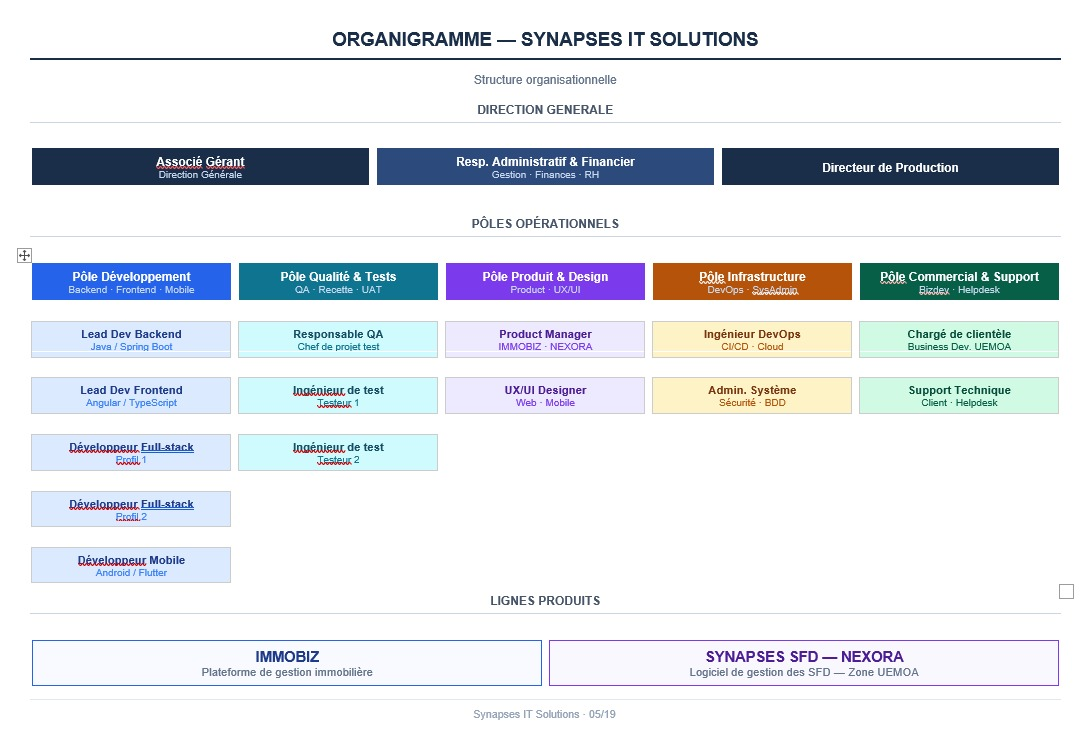
\includegraphics[width=\textwidth]{images/diagrammesyna.jpeg}
    \caption{Diagramme de l'entreprise}
    \label{fig:prospect-fiche-bien}
\end{figure}





\newpage
\subsection{Présentation de l'établissement de formation}

L'Institut de Formation aux Normes et Technologies de l'Informatique (\motcle{IFNTI}) est un établissement d'enseignement supérieur situé à Sokodé, dans le quartier Bariki.
 Créé en \important{2014} , l'IFNTI se consacre à la formation en \textbf{Informatique des Organisations}, en offrant aux étudiants des connaissances théoriques solides et des compétences pratiques adaptées aux besoins du marché du travail.

\vspace{0.3cm}


L'institut propose principalement des programmes de \textbf{Licence Professionnelle} en Informatique des Organisations, en mettant l'accent sur la \textbf{conception de bases de données}, le \textbf{développement d'applications} et la \textbf{gestion de solutions informatiques}. La réalisation de projets concrets est au cœur de cette formation. Dans le cadre de ce stage, l'IFNTI a assuré un accompagnement académique rigoureux, en suivant de près la rédaction du rapport et le développement de l'application \motcle{IMMOBIZ}, contribuant ainsi à la réussite du projet.

\subsection{Contexte du stage}

Le stage s'inscrit dans le cadre de l'obtention de la Licence Professionnelle en Informatique des Organisations. Il a pour objectif principal de mettre en pratique les connaissances acquises durant la formation, en développant une solution logicielle concrète répondant à un besoin réel dans le domaine immobilier.

\subsection{Problématique}

\begin{highlightbox}

Le secteur immobilier togolais connaît une croissance soutenue, portée par une urbanisation rapide et une demande de logements en constante augmentation, notamment dans les grands centres urbains. Pourtant, malgré ce dynamisme, le marché reste profondément marqué par des pratiques informelles et une \motcle{gestion encore largement manuelle}, qui freinent son développement et exposent ses acteurs à de nombreux risques.

\subsection{Une gestion manuelle source de dysfonctionnements}

La gestion immobilière repose encore majoritairement sur des registres physiques, des échanges informels et une faible traçabilité des opérations. Du côté des \motcle{propriétaires}, le suivi des biens s'effectue le plus souvent via des carnets de quittances manuscrits ou des échanges téléphoniques non structurés. Cette organisation rudimentaire engendre des pertes d'informations, des erreurs de gestion, des loyers impayés difficiles à retracer, ainsi que des biens vacants faute de visibilité suffisante sur le marché. En l'absence d'outils numériques adaptés, aucun propriétaire ne dispose d'une vision consolidée et fiable de son patrimoine.

\subsection{Un marché exposé à la fraude et à l'insécurité juridique}

Au-delà des erreurs de gestion, le marché immobilier togolais est confronté à des dysfonctionnements plus graves : doubles ventes de biens, fraudes documentaires, absence de vérification systématique des titres fonciers et manque de suivi fiable des transactions. Ces pratiques engendrent une \important{insécurité juridique} importante et alimentent de nombreux litiges fonciers, qui représentent une part significative des affaires traitées par les tribunaux togolais.

Cette situation est aggravée par le faible niveau de professionnalisation du secteur : sur environ \textbf{2 000 agents immobiliers} en activité au Togo, seule une infime minorité, soit à peine \textbf{20 agents}, possède une carte professionnelle reconnue par les autorités. Ce déficit massif de régulation se traduit par une maîtrise insuffisante des procédures juridiques essentielles  notamment la gestion des \textbf{mandats de vente}, la réalisation des \textbf{états des lieux} et l'\textbf{encadrement des commissions}  ainsi que par une quasi-absence de traçabilité dans les transactions financières.

\subsection{Des acteurs fragilisés par l'absence de transparence}

Les principaux acteurs du marché pâtissent directement de ces insuffisances :

\begin{itemize}
    \item Les \motcle{propriétaires} peinent à rentabiliser et sécuriser leurs biens, faute d'outils de suivi performants et d'une visibilité suffisante sur leur patrimoine.
    
    \item Les \motcle{locataires et acquéreurs potentiels} sont confrontés à un accès à l'information limité et peu fiable. La recherche d'un bien repose encore largement sur le bouche-à-oreille, des affichages rudimentaires ou des intermédiaires non certifiés, sans garantie de transparence ni de sécurité. Par ailleurs, l'absence de réglementation pleinement appliquée favorise des pratiques abusives telles que des conditions de location excessives ou des frais non encadrés, rendant l'accès au logement difficile pour une grande partie de la population.
    
    \item Les \motcle{agents immobiliers}, enfin, restent limités par des outils de gestion peu performants, une faible maîtrise du numérique et un cadre professionnel encore peu structuré.
\end{itemize}

\subsection{Des transactions financières encore peu sécurisées}

À ces problèmes s'ajoute la question des \important{moyens de paiement} : les transactions immobilières au Togo impliquent encore massivement des échanges en espèces, exposant toutes les parties à des risques de fraude, de vol et d'opacité financière. L'intégration de solutions de paiement numérique sécurisées n'est donc plus seulement une opportunité de modernisation : c'est une nécessité pour assainir durablement le secteur et lutter contre les flux financiers illicites.

\subsection{Formulation de la problématique}

Face à ce constat, la problématique centrale de ce stage peut être formulée ainsi :

\begin{quote}
\important{Comment concevoir et développer une application  intuitive et sécurisée permettant une gestion efficace des biens immobiliers, une mise en relation fiable entre propriétaires, locataires et acquéreurs, et une intégration de moyens de paiement adaptés au contexte togolais ?}
\end{quote}

Cette question soulève plusieurs enjeux complémentaires : comment centraliser et fiabiliser l'information sur les biens disponibles ? Comment garantir la sécurité juridique et financière des échanges ? Et comment concevoir une interface accessible à des utilisateurs dont la maîtrise du numérique reste hétérogène ? La digitalisation du secteur constitue ainsi une réponse structurante pour réduire les risques, optimiser la gestion des biens et moderniser un marché en pleine croissance mais encore marqué par de nombreuses insuffisances.
\end{highlightbox}
\newpage

% ===============================
% CHAPITRE 2
% ===============================
\chapter{Analyse des besoins et conception de la solution}

\subsection{Modélisation fonctionnelle}

Afin de mieux comprendre l'articulation entre les différentes vues du système \textbf{IMMOBIZ}, le tableau suivant résume le rôle de chaque diagramme utilisé lors de la phase de conception :
\begin{table}[H]
    \centering
    \begin{tabular}{|p{3cm}|p{3cm}|p{7cm}|}
        \hline
        \textbf{Diagramme} & \textbf{Type de vue} & \textbf{Objectif principal} \\ \hline
        \textbf{Cas d'utilisation} & Fonctionnelle & \textit{Qui fait quoi ?} Définit les besoins et les acteurs. \\ \hline
        \textbf{Classes} & Statique & \textit{Quelles données ?} Définit la structure de la base de données. \\ \hline
        \textbf{Séquence} & Dynamique & \textit{Comment ça circule ?} Détaille les échanges entre objets. \\ \hline
    \end{tabular}
    \caption{Comparaison des rôles des diagrammes UML dans le projet}
\end{table}

\subsection{Diagramme de cas d'utilisation (UML)}

Le diagramme de cas d'utilisation constitue la première vue de la modélisation UML. Il permet d'identifier les interactions entre les différents \textbf{acteurs} et les fonctionnalités offertes par la plateforme \textbf{IMMOBIZ}. Ce diagramme permet de fixer le périmètre fonctionnel du projet en précisant les droits et actions de chaque utilisateur.


% --- PROSPECT ---
\subsection{Cas d'utilisation : Le Prospect}

\begin{figure}[H]
    \centering
    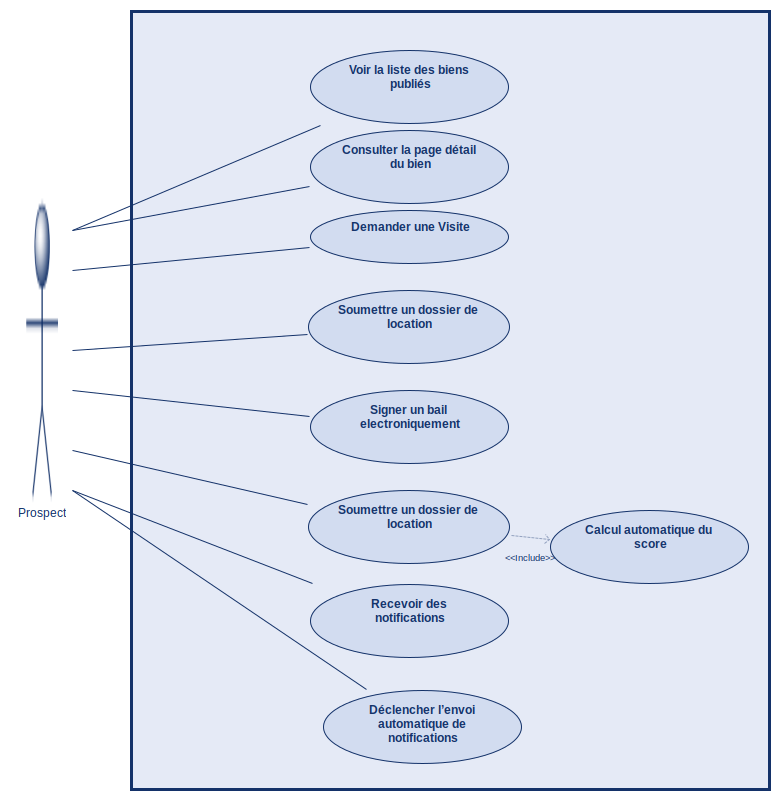
\includegraphics[width=0.9\textwidth]{images/Diagramme de cas d'utilisation Prospect.png}
    \caption{Diagramme de cas d'utilisation - Prospect}
\end{figure}







\textbf{Analyse du processus :}
Le prospect représente l'utilisateur potentiel. Le diagramme ci-dessus met en avant le parcours d'acquisition, allant de la simple consultation des annonces à la soumission du dossier. Une fonctionnalité critique ici est la \textbf{soumission du dossier de location} qui déclenche automatiquement le \textbf{calcul du score de fiabilité}.

% Le prospect peut également engager des transactions initiales telles que le paiement de la caution ou la signature électronique du bail.

% --- LOCATAIRE ---
\subsection{Cas d'utilisation : Le Locataire}

\begin{figure}[H]
    \centering
    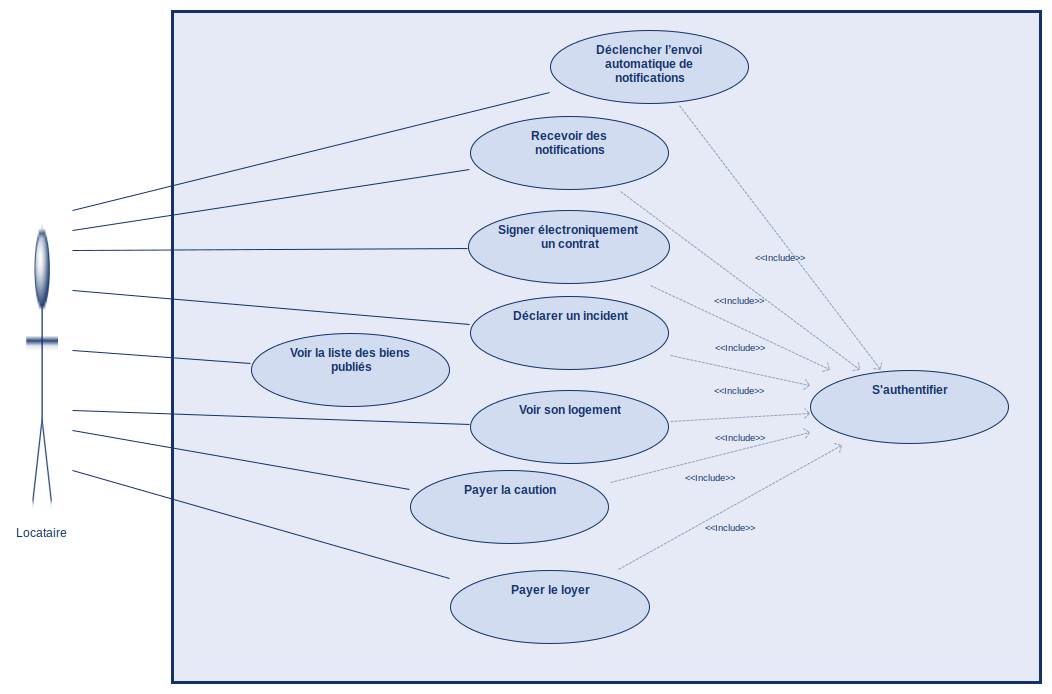
\includegraphics[width=0.9\textwidth]{images/Diagramme de cas d'utilisation Locataire Locataire.png}
    \caption{Diagramme de cas d'utilisation - Locataire}
\end{figure}


\begin{figure}[H]
    \centering
    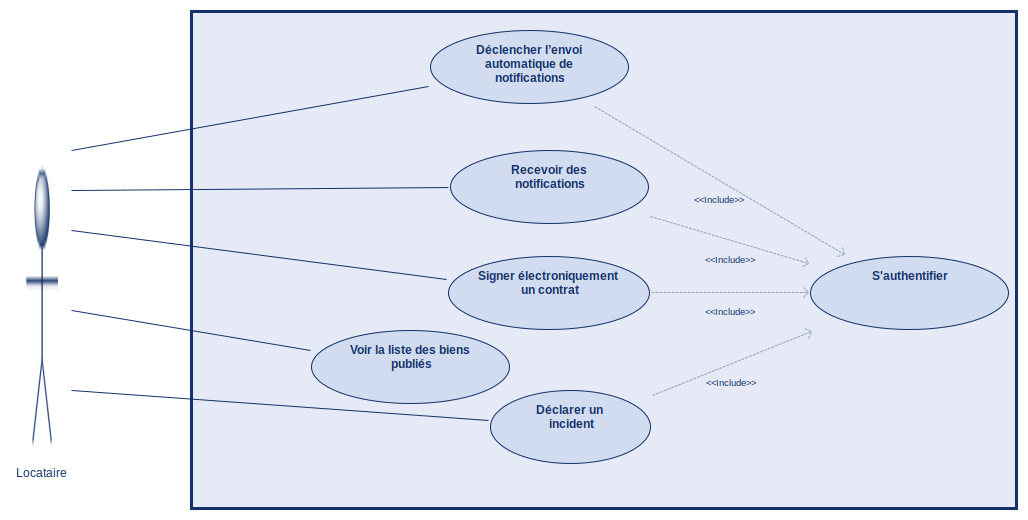
\includegraphics[width=0.9\textwidth]{images/Diagramme de cas d'utilisation Locataire Partie1.png}
        \caption{Diagramme de cas d'utilisation - Locataire}
\end{figure}


\begin{figure}[H]
    \centering
    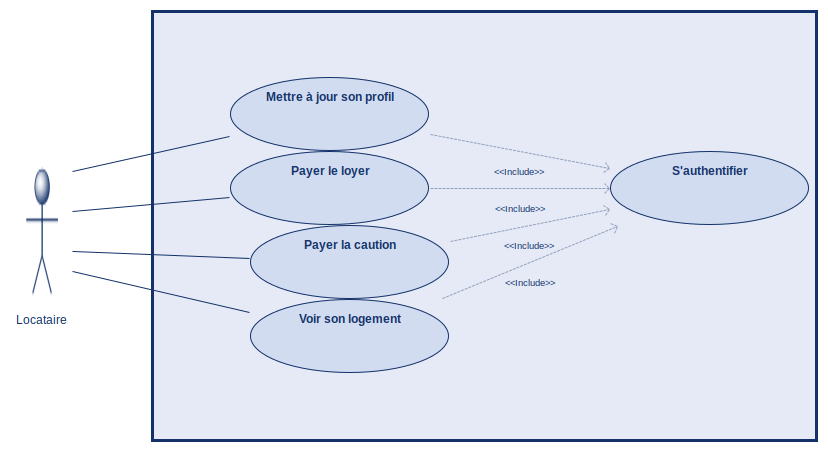
\includegraphics[width=0.9\textwidth]{images/Diagramme de cas d'utilisation Locataire Partie2.png}
    \caption{Diagramme de cas d'utilisation - Locataire}
\end{figure}

\textbf{Analyse des interactions :}
Une fois son dossier validé, l'utilisateur devient officiellement un locataire. Ses interactions se concentrent alors sur la gestion courante du bien occupé. On note que toutes les actions à forte valeur juridique ou financière (paiements, demandes d'entretien) sont liées par une relation d'inclusion (\textit{include}) à l'authentification, garantissant la sécurité et la traçabilité des opérations.
% --- PROPRIETAIRE ---




\subsection{Cas d'utilisation : Le Propriétaire et Gestionnaire}

\begin{figure}[H]
    \centering
    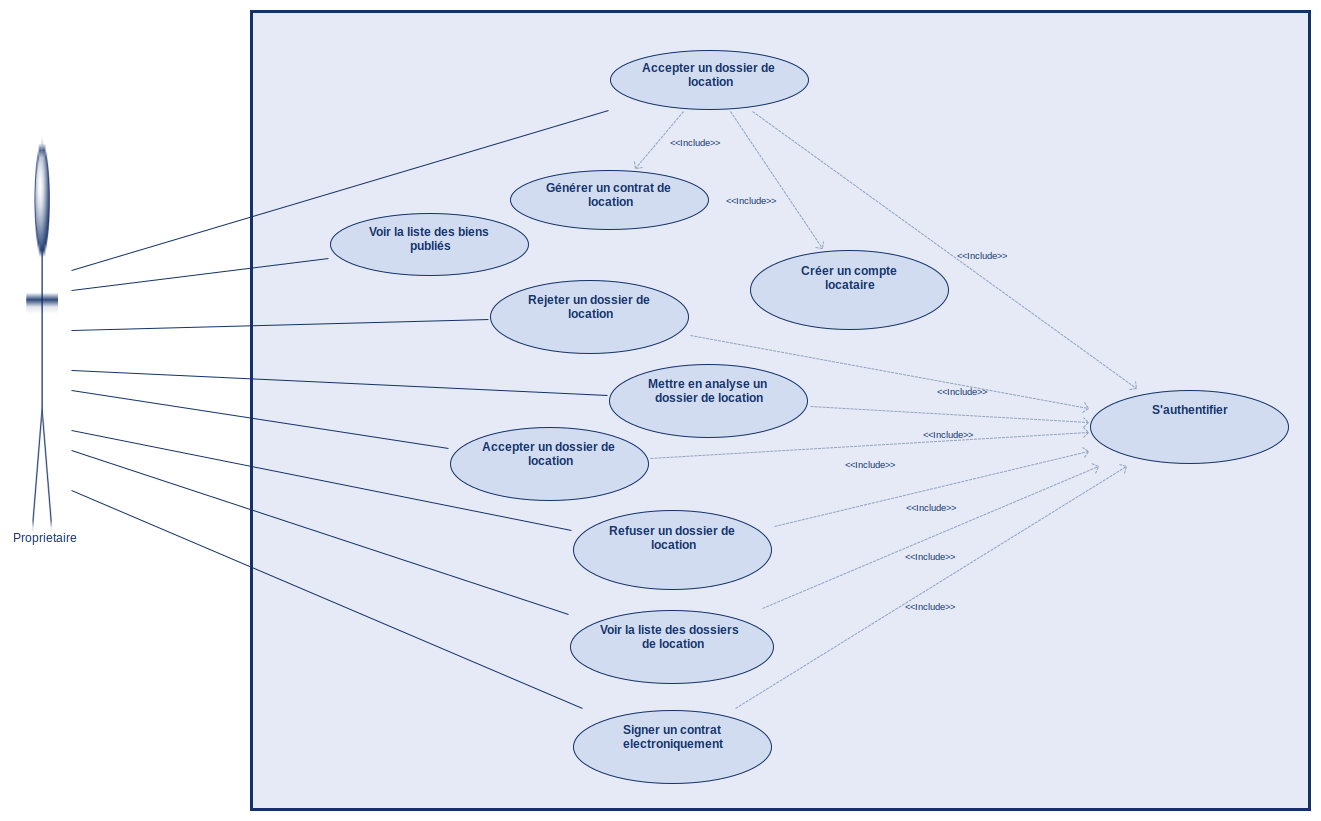
\includegraphics[width=0.9\textwidth]{images/Diagramme de cas d'utilisation immobiz Proprietaire partie1.png}
    \caption{Diagramme de cas d'utilisation - Propriétaire}
\end{figure}


\begin{figure}[H]
    \centering
    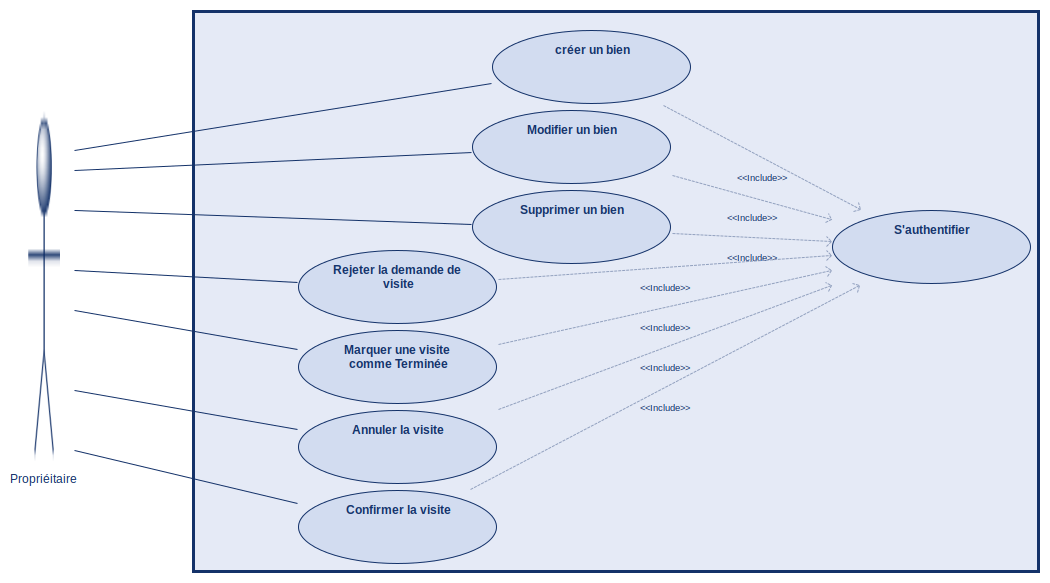
\includegraphics[width=0.9\textwidth]{images/Diagramme de cas d'utilisation immobiz partie2.png}
    \caption{Diagramme de cas d'utilisation - Propriétaire}
\end{figure}


\begin{figure}[H]
    \centering
    
    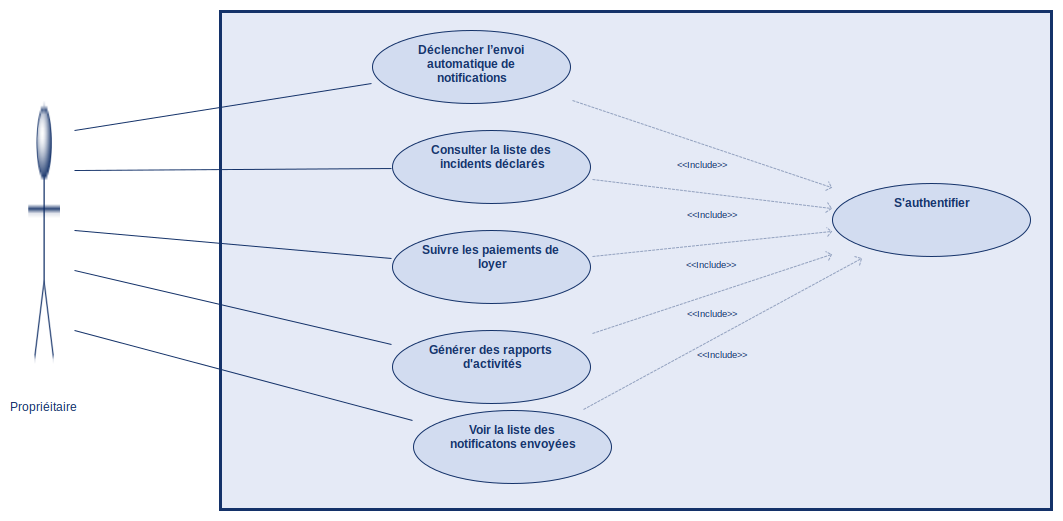
\includegraphics[width=0.9\textwidth]{images/Diagramme de cas d'utilisation immobiz Proprietaire partie3.png}
    \caption{Diagramme de cas d'utilisation - Propriétaire}
\end{figure}

\textbf{Analyse des responsabilités :}

Le propriétaire et le gestionnaire disposent des principales fonctionnalités de gestion de la plateforme \motcle{IMMOBIZ}. Ils peuvent administrer les biens immobiliers, suivre les visites, consulter les incidents, gérer les dossiers de location, suivre les paiements de loyer et générer des rapports d'activité. Ils interviennent également dans le traitement des candidatures locatives, la validation ou le refus des dossiers ainsi que la gestion des contrats de location. Toutes ces opérations nécessitent une authentification préalable afin de garantir la sécurité et la traçabilité des actions effectuées sur la plateforme.







% --- SYSTEME ---
\subsection{Cas d'utilisation : Gérant Immobiz}

Le diagramme de cas d'utilisation du \textbf{Gérant Immobiz} présente les principales fonctionnalités accessibles à cet acteur au sein de la plateforme immobilière. Le gérant joue un rôle central dans l'administration, le suivi et le contrôle des activités de la plateforme.

Ses responsabilités incluent la gestion des utilisateurs à travers l'activation et la désactivation des comptes utilisateurs. Il assure également l'administration des rôles en créant, modifiant ou supprimant les différents rôles attribués aux utilisateurs.

Le gérant dispose d'un accès aux informations opérationnelles de la plateforme, notamment la consultation de la liste des biens publiés, des demandes de visite, des dossiers de location, des contrats, des incidents signalés ainsi que des notifications générées par le système.

Par ailleurs, il est chargé de la planification des interventions nécessaires au bon fonctionnement des services et peut consulter les journaux d'audit ainsi que les journaux d'activités afin de garantir la traçabilité et la sécurité des opérations effectuées sur la plateforme.

Enfin, le gérant a accès aux statistiques des opérations de la plateforme, lui permettant d'analyser les performances, de suivre les activités des utilisateurs et de prendre des décisions stratégiques basées sur des données fiables.

L'ensemble de ces fonctionnalités nécessite au préalable une authentification de l'utilisateur, ce qui garantit un accès sécurisé aux ressources et aux données de la plateforme.

\begin{figure}[H]
    \centering
    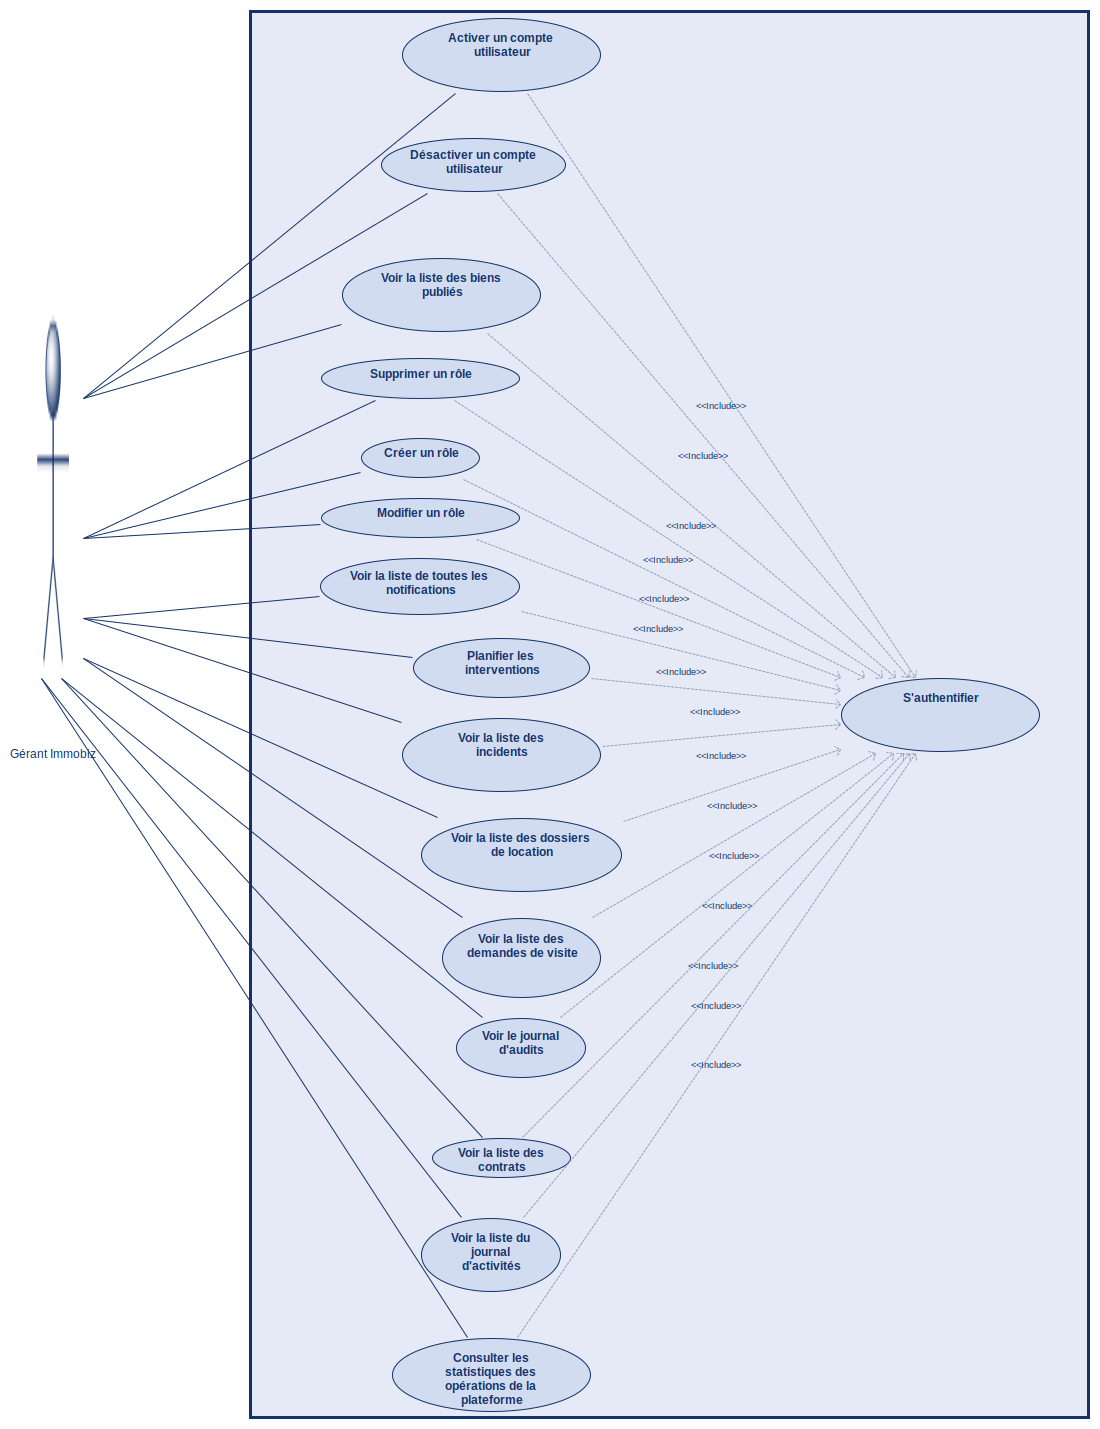
\includegraphics[width=0.9\textwidth]{images/Diagramme de cas d'utilisation GérantImmobiz.png}
    \caption{Diagramme de cas d'utilisation - Gérant Immobiz}
\end{figure}

\vspace{0.6cm}



\newpage
\subsection{Diagramme de cas d'utilisation du Technicien}

Le diagramme de cas d'utilisation du technicien illustre l'ensemble des 
actions qu'il peut effectuer sur la plateforme \motcle{IMMOBIZ}. Son 
périmètre d'action est centré sur la gestion des incidents signalés par 
les locataires : de la prise en charge jusqu'à la clôture, en passant 
par la rédaction du rapport d'intervention. Toutes les actions sensibles 
nécessitent une authentification préalable.

\begin{figure}[H]
    \centering
    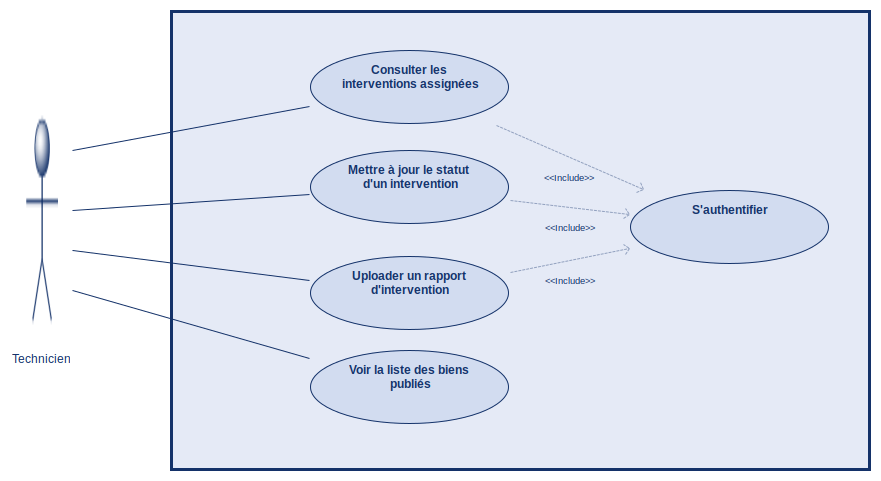
\includegraphics[width=\textwidth]{images/Diagramme de cas d'utilisation immobiz Technicien.png}
    \caption{Diagramme de cas d'utilisation du Technicien}
    \label{fig:uml-technicien}
\end{figure}




\newpage
\subsection{Diagramme de cas d'utilisation de l'Agence Immobilière}

Le diagramme de cas d'utilisation de l'agence immobilière illustre l'ensemble
des actions qu'elle peut effectuer sur la plateforme \motcle{IMMOBIZ}. Son
périmètre d'action est large et couvre la gestion des biens, des gestionnaires,
des demandes de location, des contrats, des visites, des interventions et des
documents. Elle dispose également d'un accès aux rapports, aux notifications
envoyées et aux demandes de maintenance, lui permettant ainsi d'avoir une vue
d'ensemble complète sur l'activité de la plateforme. Toutes ces actions
nécessitent une authentification préalable.
\begin{figure}[H]
    \centering
    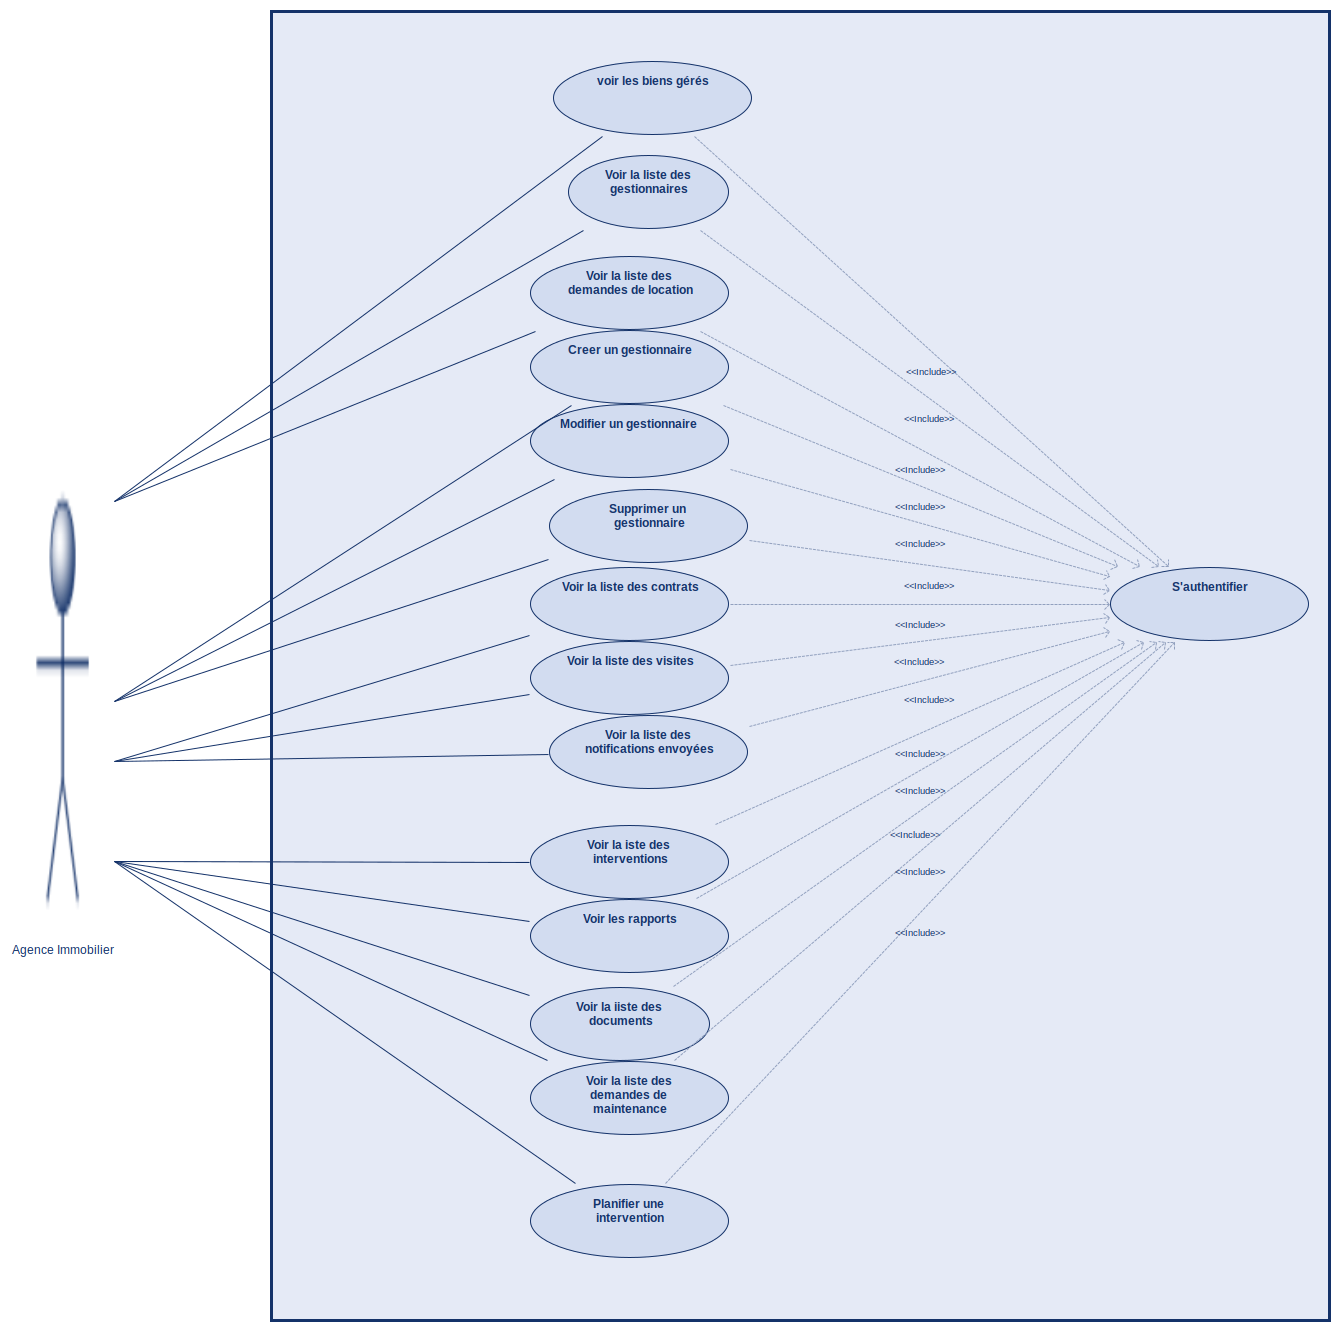
\includegraphics[width=\textwidth]{images/Diagramme de cas d'utilisation immobiz Agence Immobiliere.png}
    \caption{Diagramme de cas d'utilisation de l'Agence Immobilière}
    \label{fig:uml-technicien}
\end{figure}







\newpage
\subsubsection dynamique (Scénarios d'exécution)}

Si les diagrammes de cas d'utilisation définissent les fonctionnalités, les scénarios d'exécution permettent d'illustrer la chronologie des échanges. Cette étape permet de visualiser les échanges entre le \important{Front-end (Angular)} et le \important{Back-end (Spring Boot)} pour les flux les plus critiques du système.

% --- SCENARIO 1 : SCORING ---
\subsection{Scénario d'exécution : Soumission de dossier et scoring automatique}

Le schéma suivant décrit le parcours d'un dossier dès sa soumission par le prospect jusqu'à sa mise à disposition pour le propriétaire.

\begin{figure}[H]
    \centering
    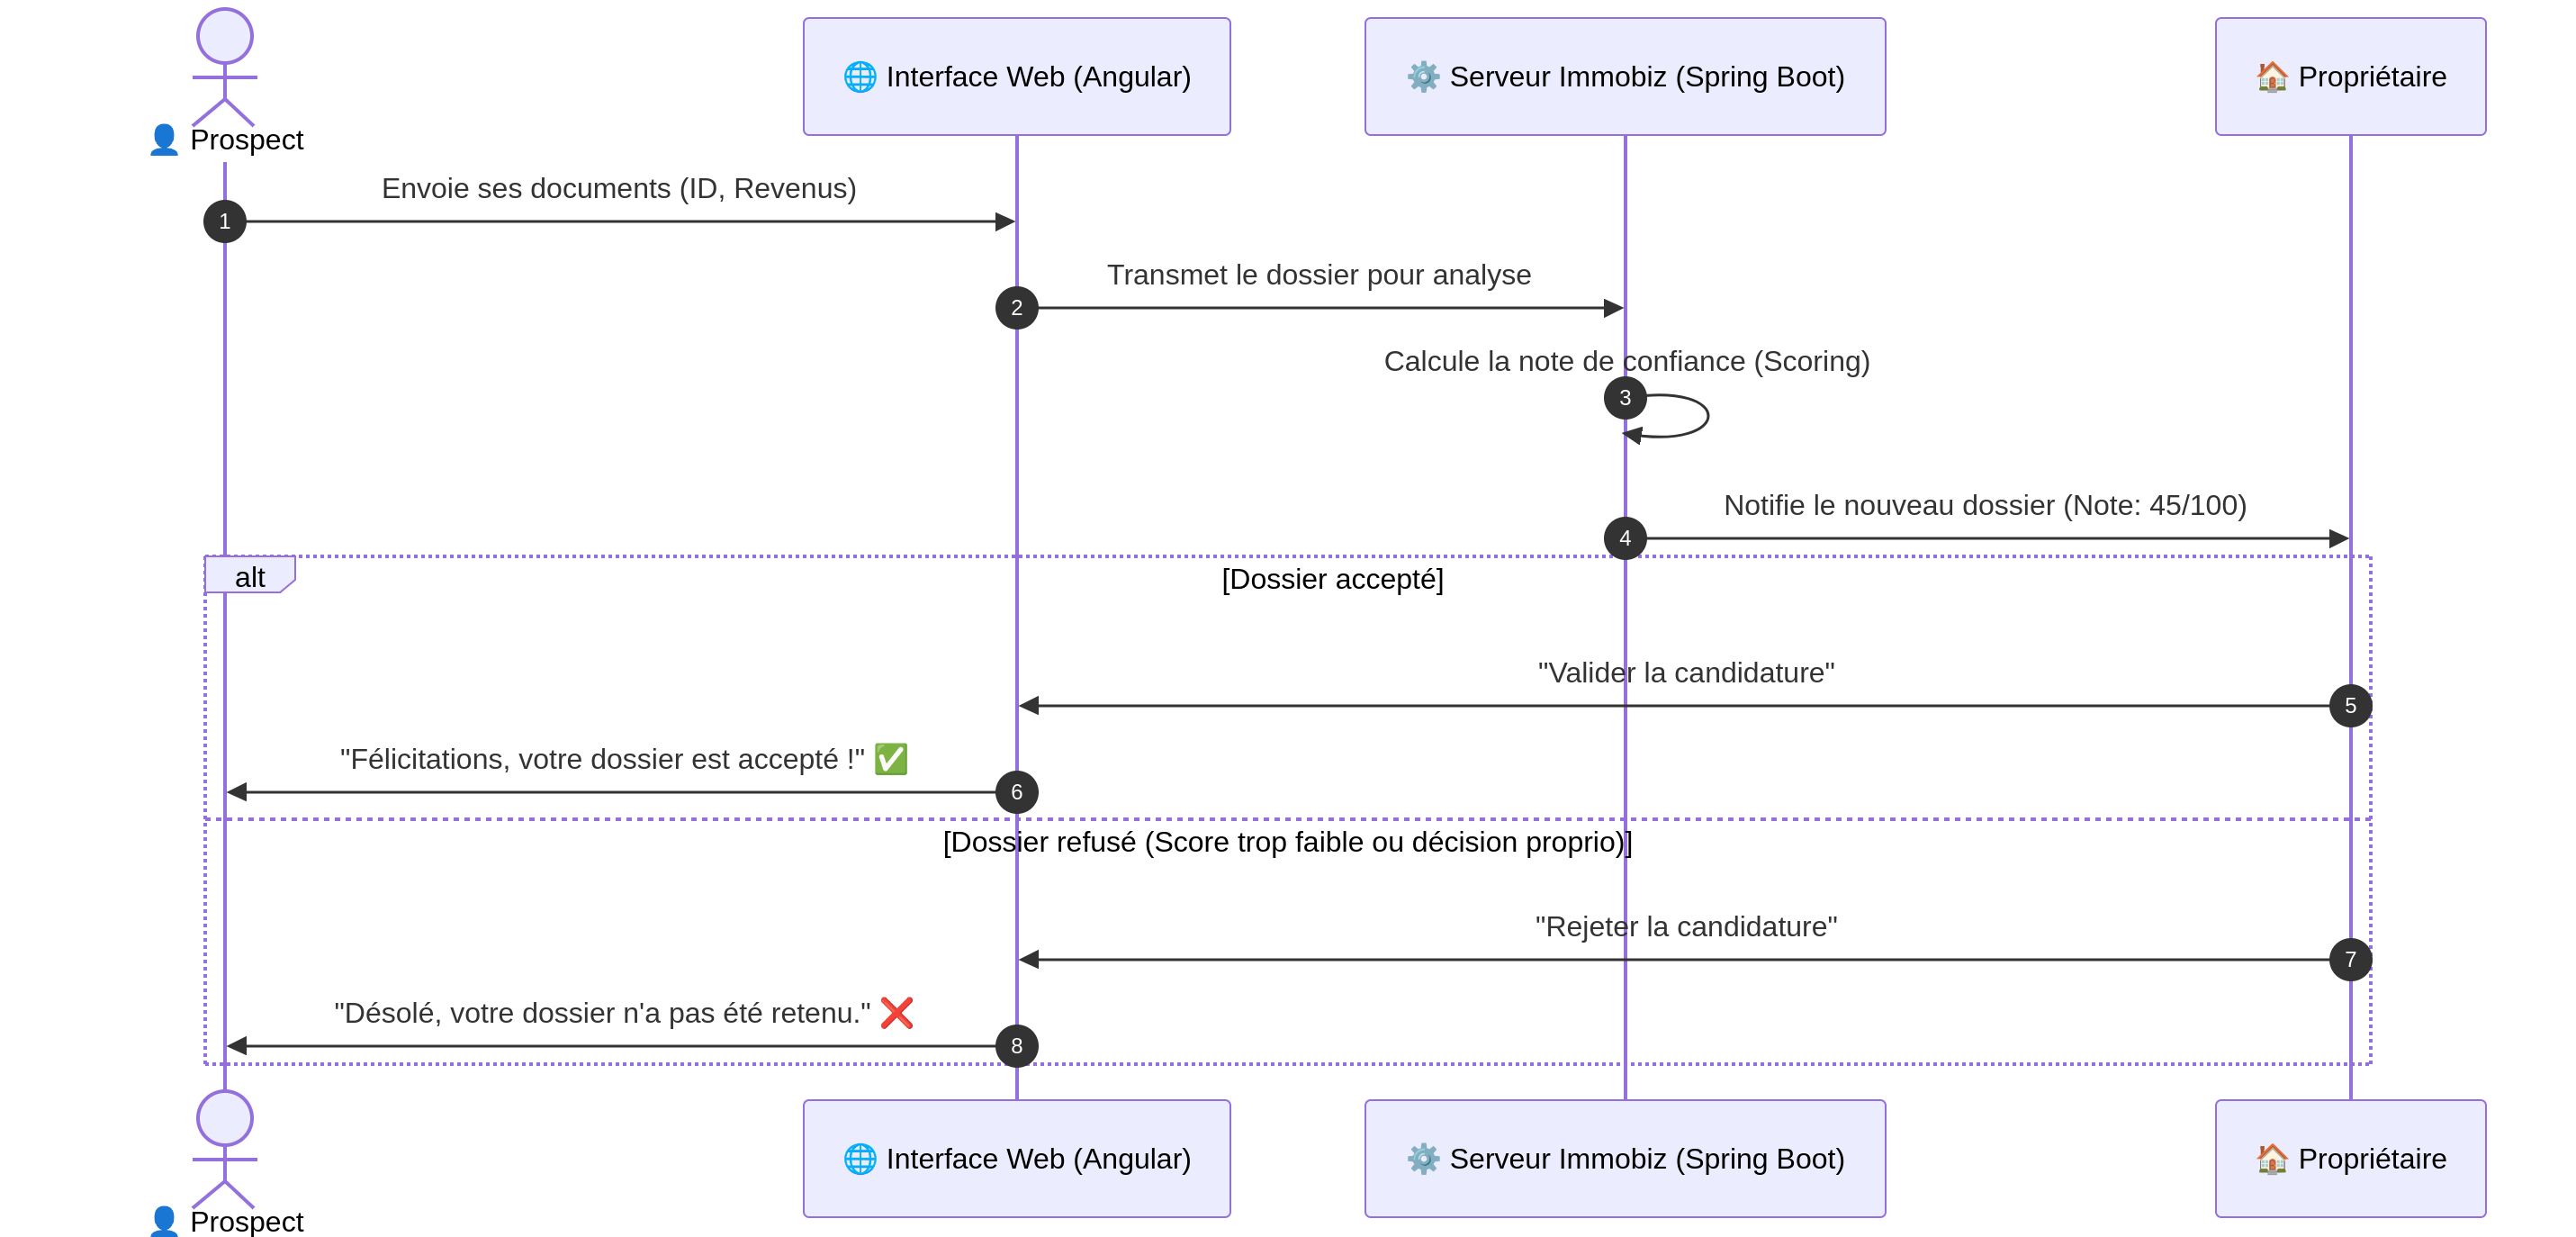
\includegraphics[width=0.9\textwidth]{images/sequence-uppload-doc.png}
    \caption{Scénario d'exécution : Soumission de dossier et scoring automatique}
    \label{fig:scen_scoring}
\end{figure}

\textbf{Analyse du flux de scoring :}
\begin{itemize}[label=\textbullet]
    \item \motcle{Automatisation :} Dès le téléversement des justificatifs sur l'interface \textbf{Angular}, le back-end traite les données via une API REST sécurisée vers le serveur \textbf{Spring Boot}.
    \item \motcle{Aide à la décision (Fragment alt) :} Le système génère un score automatique. Pour modéliser les deux issues possibles de l'évaluation, le diagramme utilise une structure conditionnelle \textbf{alt} (\textit{Alternative}) qui sépare les flux selon le résultat : 
    \begin{itemize}
        \item \textbf{Cas de succès [Score $\ge$ Seuil] :} Si le score est suffisant et que le propriétaire valide, le prospect reçoit une confirmation immédiate et le système prépare l'édition du bail.
        \item \textbf{Cas de refus [Score < Seuil] :} Si le score est trop faible ou les pièces jugées insuffisantes, le système exécute la branche alternative du bloc. Il notifie automatiquement le prospect du rejet de sa candidature, libérant ainsi instantanément le bien pour d'autres postulants.
    \end{itemize}
    \item \motcle{Notification et Transparence :} Ce flux, orchestré par le fragment \textbf{alt}, garantit une réactivité optimale. Il évite aux prospects une attente inutile tout en offrant au propriétaire une aide au choix objective et rapide.
\end{itemize}
\newpage
% --- SCENARIO 2 : PAIEMENT ---
\subsection{Scénario d'exécution : Règlement multi-canal de la caution}

L'intégration des services financiers numériques est un pilier de la sécurisation des transactions au sein de la plateforme.

\begin{figure}[H]
    \centering
    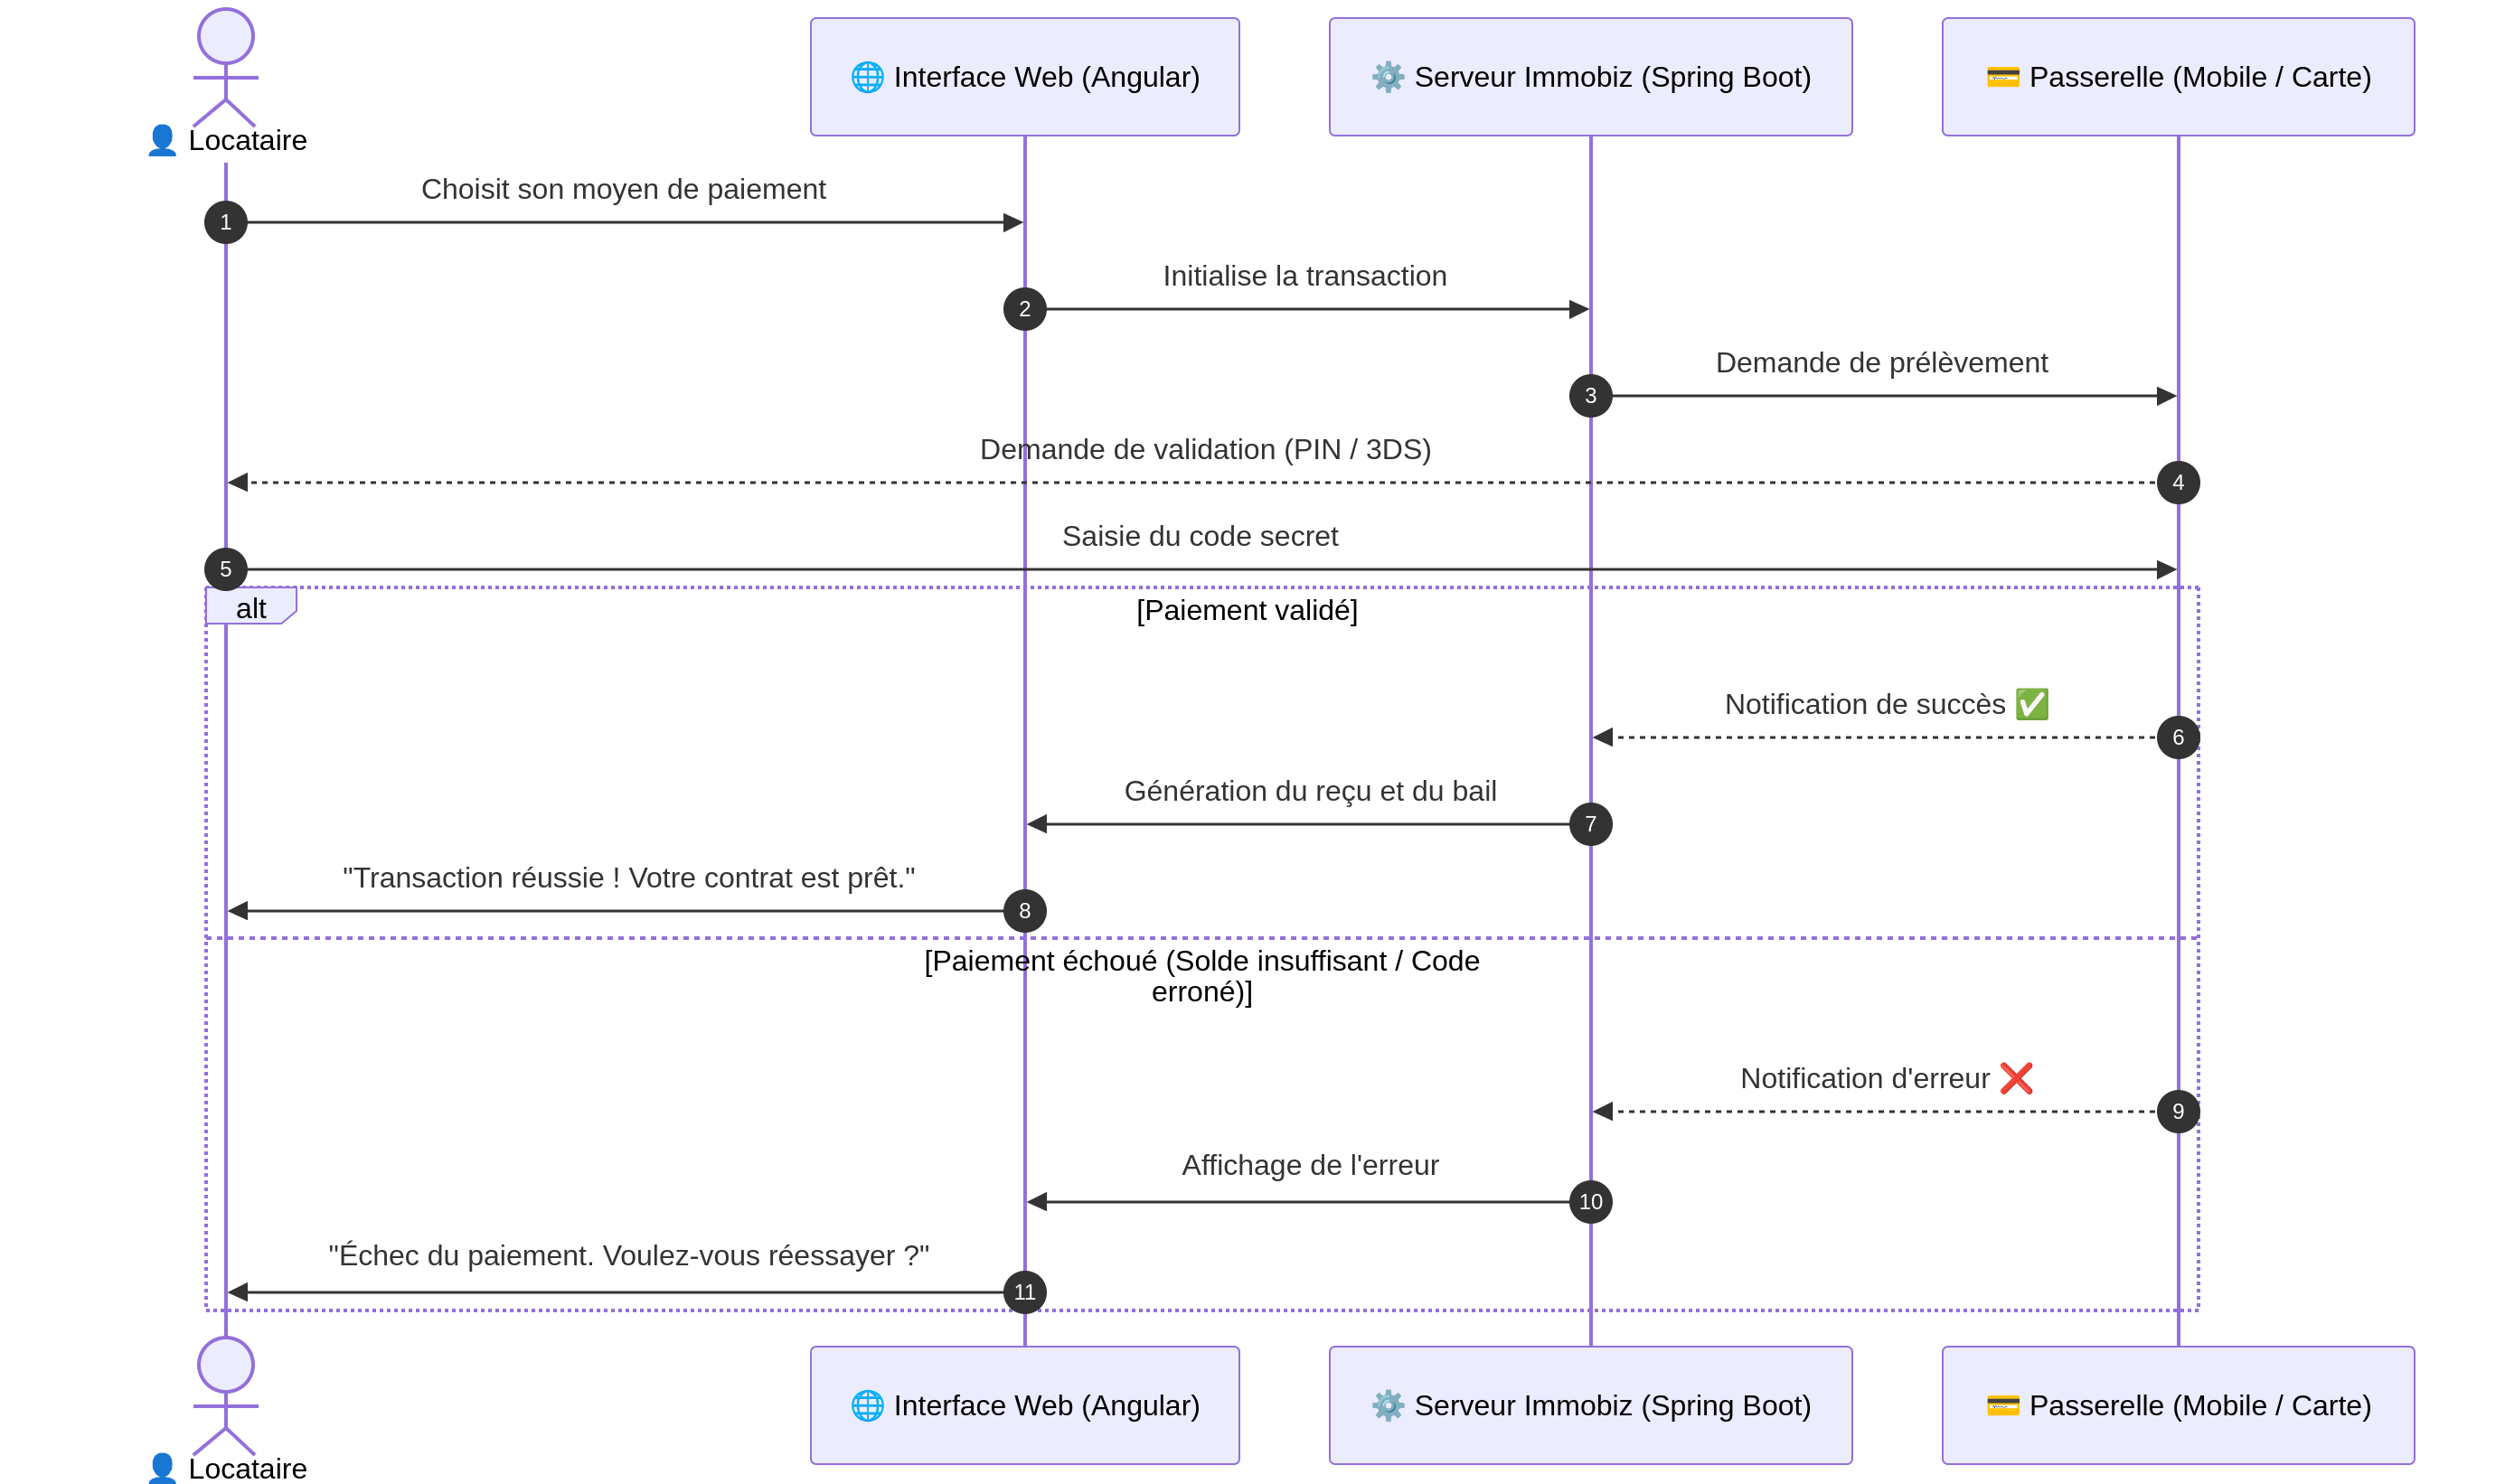
\includegraphics[width=0.9\textwidth]{images/sequence-payement1.png}
    \caption{Scénario d'exécution : Processus de paiement de la caution}
    \label{fig:scen_paiement}
\end{figure}
\textbf{Analyse du flux de paiement (Gestion des exceptions) :}

La fiabilité du système repose sur sa capacité à traiter les imprévus lors des transactions financières, un aspect modélisé par le fragment combiné \textbf{alt}.

\begin{itemize}[label=\textbullet]
    \item \motcle{Structure Alternative (alt) :} L'utilisation du bloc \textbf{alt} dans le diagramme de séquence est fondamentale pour la robustesse de l'application. Elle permet de définir deux scénarios s'excluant mutuellement selon le retour de la passerelle de paiement : un chemin nominal (succès) et un chemin d'exception (échec). Cela garantit que le système réagit de manière déterministe à chaque réponse du prestataire.

    \item \motcle{Sécurisation et Validation :} Le diagramme illustre le point de contrôle critique où le prestataire de paiement (Mixx by yas, Flooz ou Banque) demande une validation (PIN ) pour confirmer la disponibilité des fonds et l'identité de l'utilisateur.

    \item \motcle{Traitement des scénarios :}
    \begin{itemize}
        \item \textbf{Scénario de Succès :} Une fois la notification reçue, le serveur \textbf{Spring Boot} confirme la transaction. Cela déclenche automatiquement la mise à jour de la base de données, la génération du reçu et du bail, ainsi que la notification positive sur l'interface \textbf{Angular}.
        \item \textbf{Scénario d'Échec :} En cas de solde insuffisant, de code erroné ou d'annulation, le système intercepte l'erreur via la passerelle. L'utilisateur est immédiatement informé par un message explicite, lui permettant de renouveler sa tentative ou de changer de moyen de paiement sans perte de données.
    \end{itemize}

    \item \motcle{Intégrité des données :} Cette approche garantit la cohérence du système : le statut du contrat de bail et du bien immobilier ne bascule vers la validation définitive qu'après une confirmation de succès formelle et sécurisée.
\end{itemize}
\newpage


% --- DIAGRAMME DE CLASSE ---
\subsection{Modélisation statique}

La phase de conception de la base de données est cruciale pour garantir l'intégrité et la cohérence des données au sein de l'application \textbf{IMMOBIZ}. Elle repose sur une modélisation rigoureuse des entités et de leurs relations.



\subsection{Diagramme de classes (UML)}

Le diagramme de classes constitue la représentation statique du système. Il définit les entités métiers, leurs attributs ainsi que les liens de dépendance et d'association qui les unissent. Dans notre architecture, ce diagramme sert de plan directeur pour la génération des tables de la base de données via l'ORM d'Hibernate.

\begin{figure}[H]
    \centering
    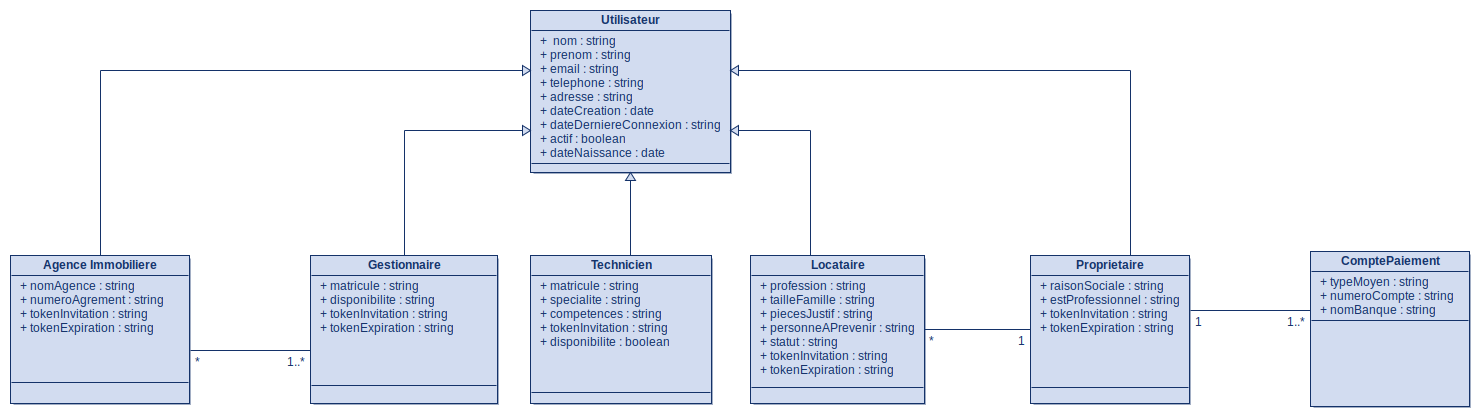
\includegraphics[width=\textwidth]{images/Diagramme de classe immobiz utilisateur.png}
    \caption{Diagramme de classes - utilisateur}
\end{figure}

\begin{figure}[H]
    \centering
    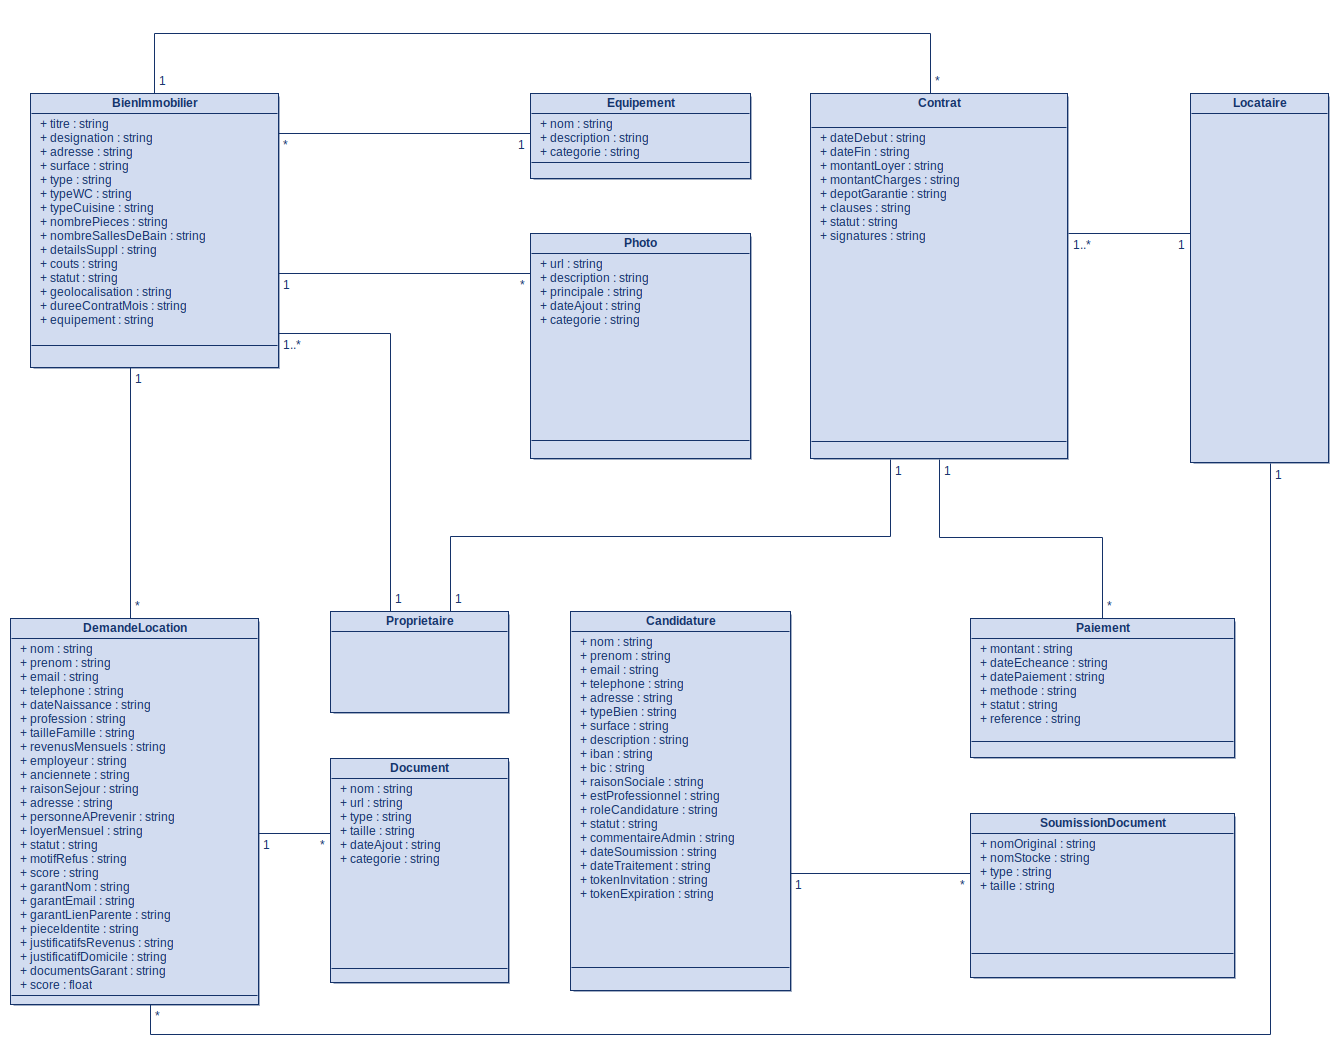
\includegraphics[width=\textwidth]{images/bien-location.png}
    \caption{Diagramme de classes - BienImmobilier et Location}
\end{figure}



\begin{figure}[H]
    \centering
    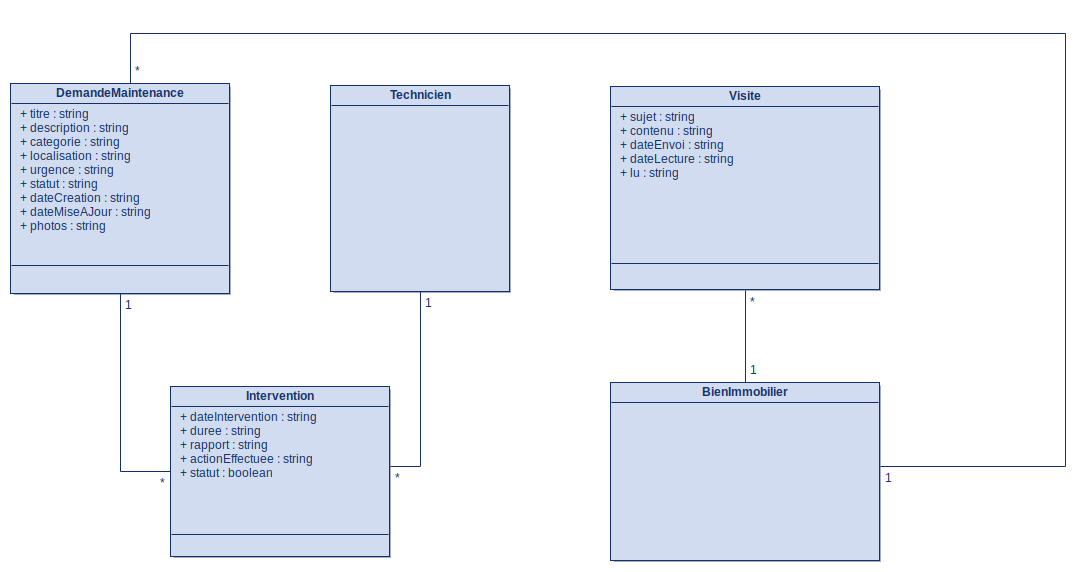
\includegraphics[width=\textwidth]{images/Diagramme de classe immobiz Gestion opérationnelle.png}
    \caption{Diagramme de classes -Gestion opérationnelle}
\end{figure}









\textbf{Analyse approfondie de la structure :}
\begin{itemize}
\item \textbf{Gestion des identités :} L'utilisation de l'héritage entre \texttt{Utilisateur} et les classes \texttt{Locataire} / \texttt{Propriétaire} permet de mutualiser les propriétés communes.
\item \textbf{Sécurisation et modularité des paiements :} Le système repose sur une entité dédiée, \texttt{ComptePaiement}, pour isoler les informations sensibles du profil général du \texttt{Propriétaire}. Cette approche permet non seulement de sécuriser les données transactionnelles, mais aussi d'offrir au bailleur la possibilité de gérer plusieurs modes de règlement (RIB pour les virements, \textbf{Mobile Money} tels que \textbf{Flooz} ou \textbf{Mixx by yas}, ou Carte Bancaire) de manière indépendante.
\item \textbf{Cycle de vie de la location :} Le \texttt{BienImmobilier} est au centre du processus. Le \texttt{Bail} fait office de pivot contractuel liant le bien et le locataire, tout en portant les paramètres financiers tels que la caution et le loyer.
\item \textbf{Flux financiers et traçabilité :} Le lien entre \texttt{Bail} et \texttt{Paiement} assure une traçabilité rigoureuse : chaque règlement (Caution, Loyer mensuel ou Frais de dossier) est directement rattaché au contrat de bail correspondant. Cela permet un suivi en temps réel des impayés et de l'historique financier de chaque location.
\item \textbf{Suivi technique :} La classe \texttt{Intervention} permet un suivi historique des incidents et des maintenances déclarés sur les biens immobiliers.
\item \textbf{Solidité documentaire et Scoring :} La cardinalité $1..*$ entre \texttt{DossierLocation} et \texttt{Document} garantit que chaque dossier est constitué de l'ensemble des pièces justificatives requises (Identité, Revenus, etc.). Ces données alimentent le \texttt{scoreAutomatique}, un algorithme qui évalue la fiabilité du candidat sur une base de 100 points pour sécuriser la mise en location.
\end{itemize}  


% ===============================
% CHAPITRE 3
% ===============================
\chapter{Réalisation et résultats}
\subsection{Présentation générale de la solution}
\begin{highlightbox}
\motcle{IMMOBIZ} est une application web de gestion immobilière qui facilite 
la mise en relation entre locataires et propriétaires, tout en offrant au gérant un contrôle global sur la plateforme. Elle centralise la gestion des biens, des annonces et des réservations, et permet un suivi clair et rapide des interactions entre les utilisateurs.

\vspace{0.3cm}

La solution vise à simplifier le processus de recherche et de location de biens immobiliers, à sécuriser les échanges et à offrir une interface intuitive pour tous les types d'acteurs de la plateforme. %De plus, IMMOBIZ 
%propose des \important{moyens de paiement intégrés}, afin de %faciliter les 
%transactions entre locataires et propriétaires de manière %sécurisée et 
%transparente.


\vspace{0.3cm}
Sur le plan technique, la solution repose sur une architecture moderne 
découplée : le \important{front-end} est développé avec \motcle{Angular}, 
offrant une interface réactive et maintenable grâce à la gestion d'état 
centralisée via des \important{Stores}, utilisés lors de la consommation des 
APIs pour synchroniser les données entre les composants. Le \important{back-end} 
est quant à lui construit avec \motcle{Spring Boot}, en suivant une 
architecture en couches rigoureuse articulée autour des patterns 
\important{Entité}, \important{Repository}, \important{Service}, 
\important{Controller}, \important{DTO} et \important{Mapper}, garantissant 
une séparation claire des responsabilités et une meilleure maintenabilité 
du code.

\vspace{0.3cm}

Pour la gestion de l'authentification et de la sécurité, nous avons opté 
pour la bibliothèque \motcle{com.kodzotech:security-oauth2} plutôt que 
d'implémenter un mécanisme de sécurité personnalisé. Ce choix s'explique 
par plusieurs raisons : cette bibliothèque encapsule les meilleures 
pratiques de sécurité OAuth2 et JWT, réduit considérablement le risque 
d'introduire des vulnérabilités liées à une implémentation manuelle, et 
accélère le développement en fournissant des composants éprouvés et 
préconfigurés. Implémenter soi-même un système d'authentification sécurisé 
est une tâche complexe et sensible qui nécessite une expertise pointue ; 
déléguer cette responsabilité à une bibliothèque spécialisée permet à 
l'équipe de se concentrer sur la logique métier propre à \motcle{IMMOBIZ}.
\end{highlightbox}

\newpage
\subsection{Interface de l'application}

Afin d'illustrer concrètement le fonctionnement de la solution, nous 
présentons ci-dessous les principales interfaces de l'application 
\motcle{IMMOBIZ}, en suivant le parcours naturel d'un utilisateur . %depuis 
%sa première visite jusqu'à la finalisation d'une transaction.

\subsection{Page d'accueil}


La page d'accueil constitue le premier point de contact entre l'utilisateur 
et la plateforme \motcle{IMMOBIZ}. Accessible à tout visiteur sans 
authentification préalable, elle offre une vue d'ensemble des fonctionnalités 
disponibles, met en avant les biens immobiliers en vedette .%et invite 
%l'utilisateur à s'inscrire ou à se connecter pour accéder aux 
%fonctionnalités sensibles de la plateforme.

\begin{figure}[H]
    \centering
    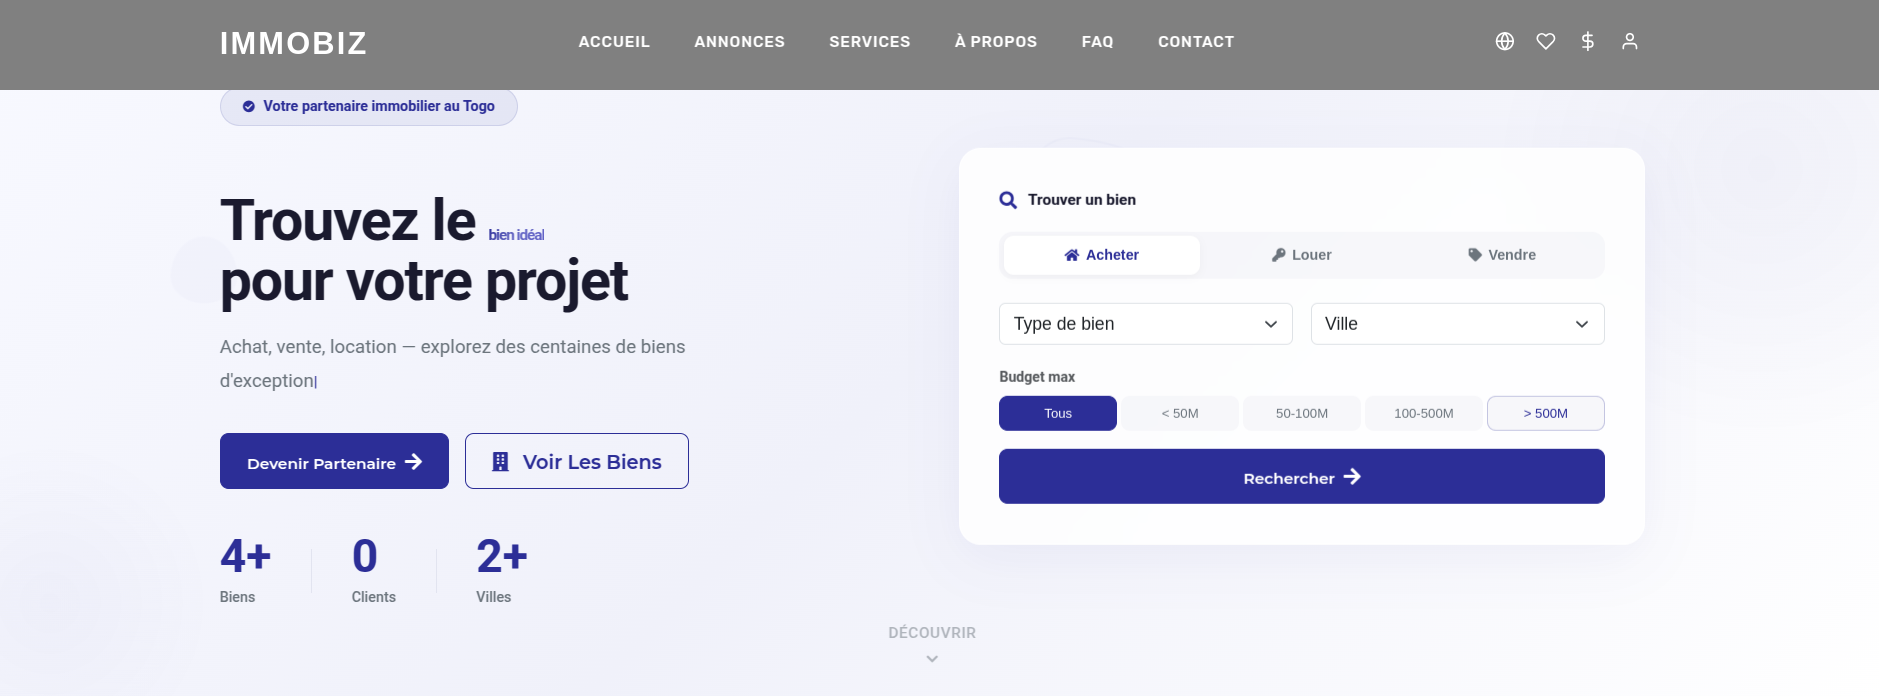
\includegraphics[width=\textwidth]{images/acueil1.png}
      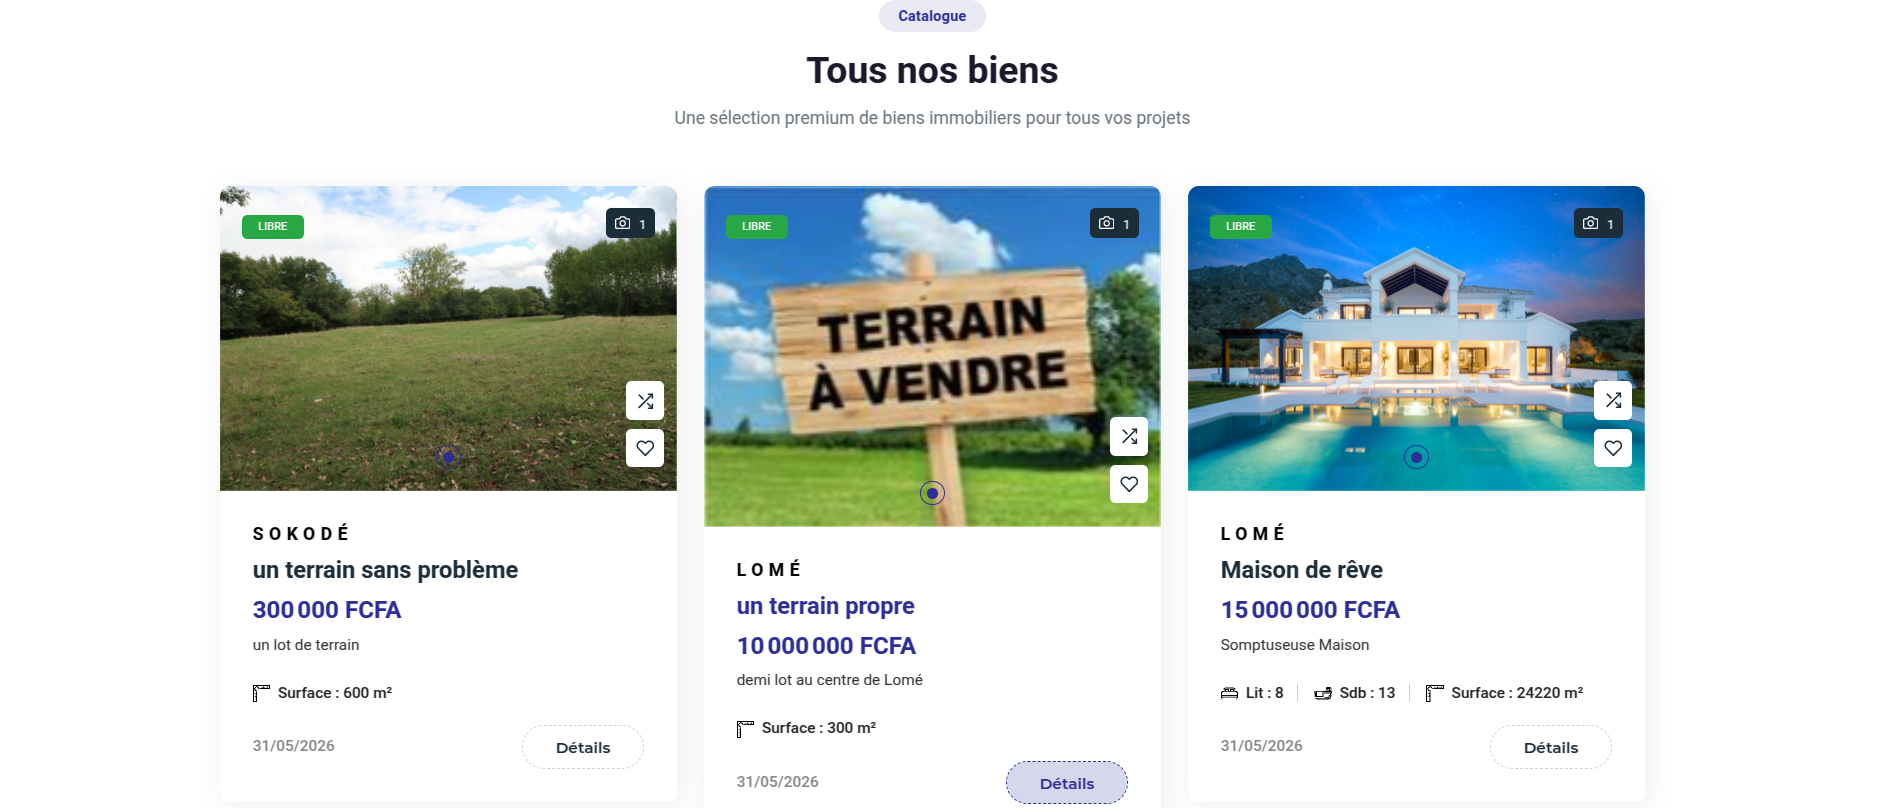
\includegraphics[width=\textwidth]{images/acueil2.png}
    \caption{Page d'accueil de l'application IMMOBIZ}
    \label{fig:accueil-1}
\end{figure}

\newpage



\begin{figure}[H]
    \centering
  
 
    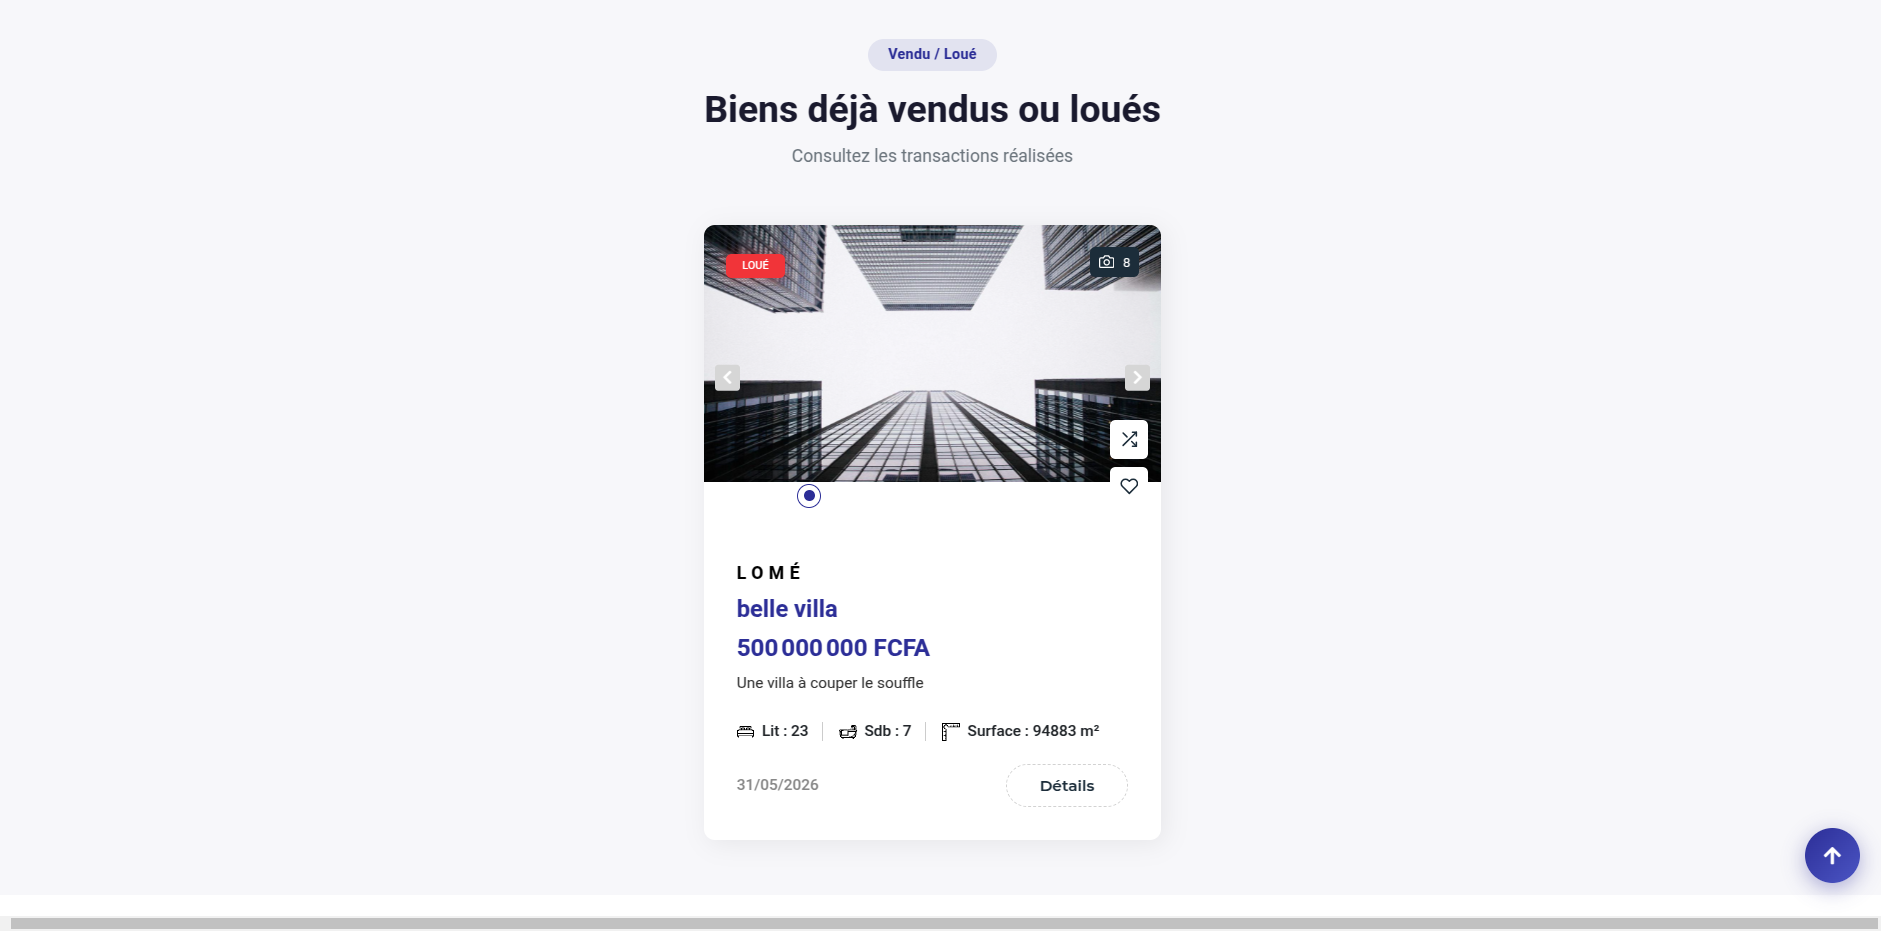
\includegraphics[width=\textwidth]{images/acueil3.png}
       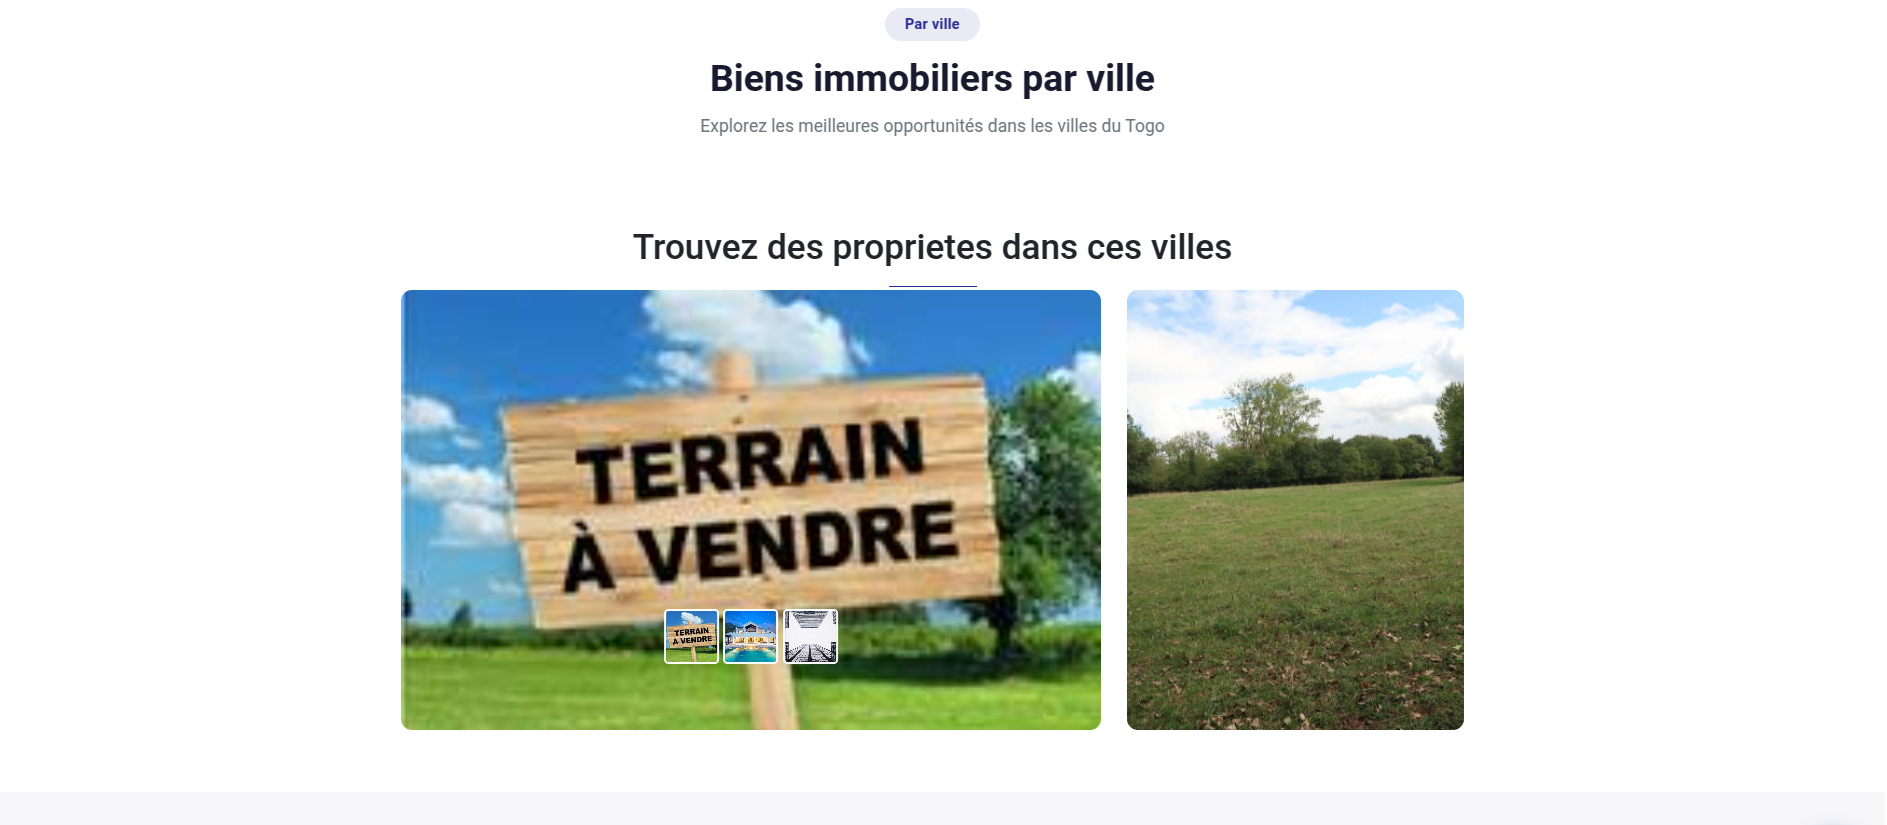
\includegraphics[width=\textwidth]{images/acueil4.png}
        
    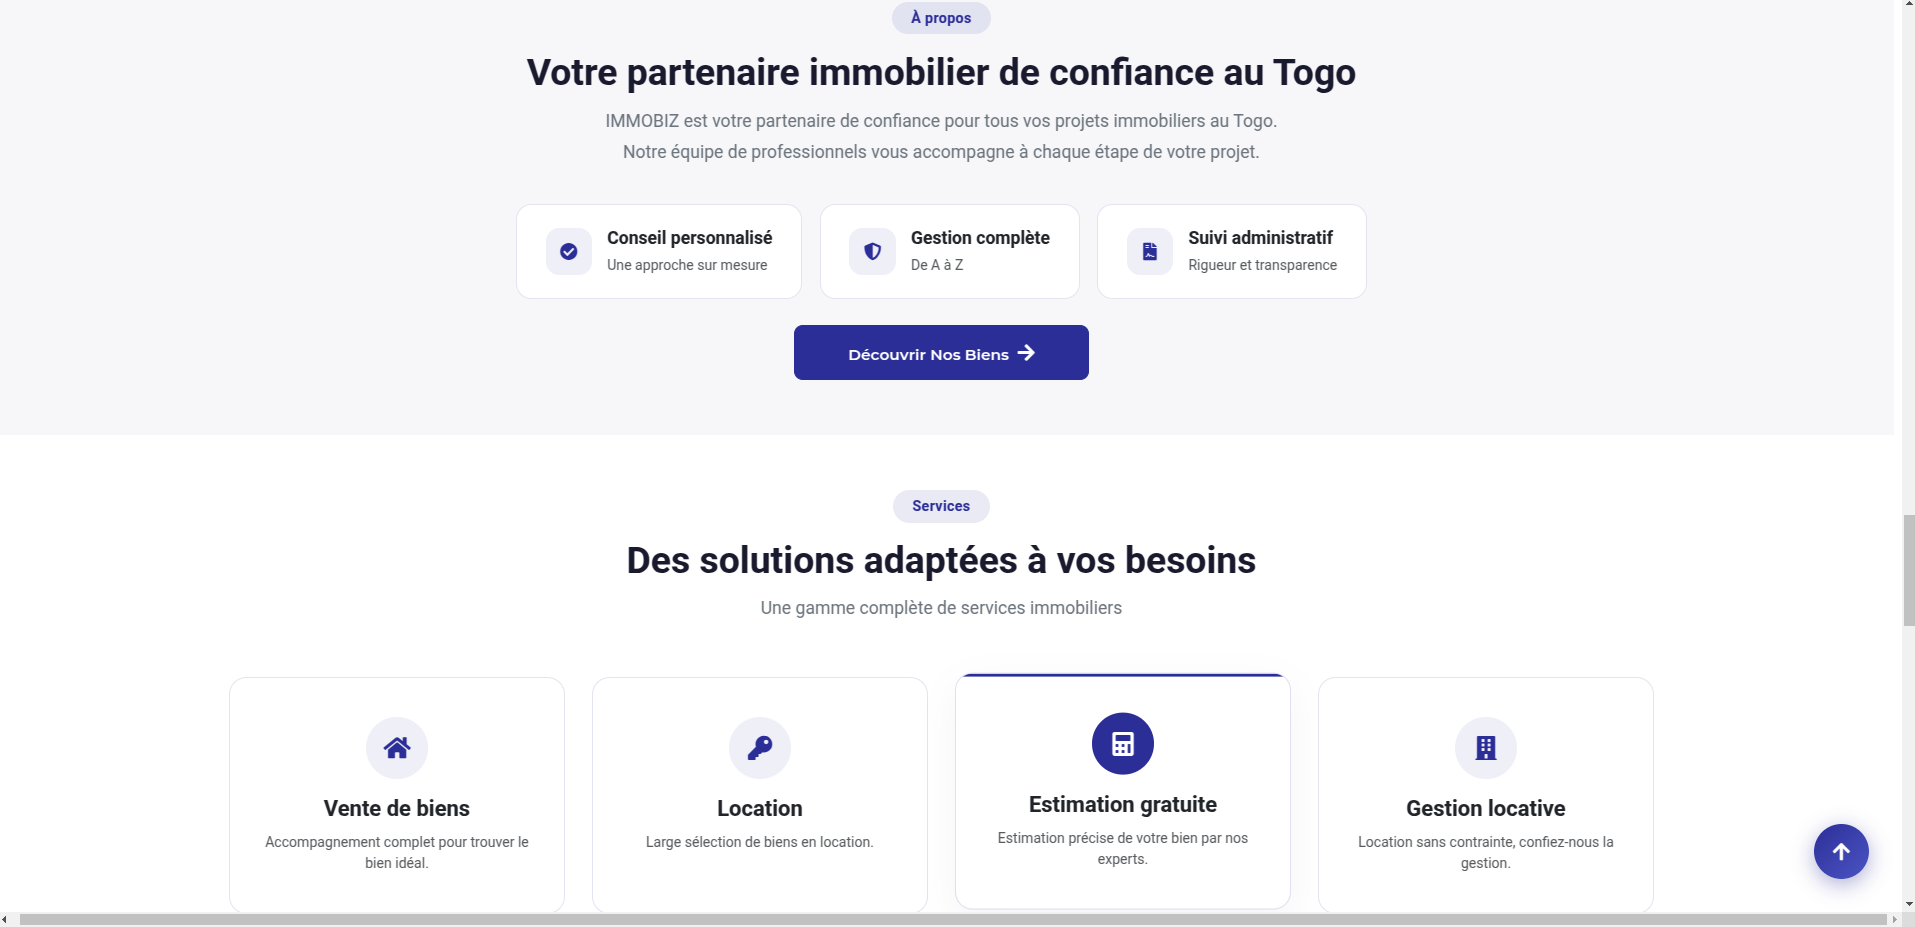
\includegraphics[width=\textwidth]{images/acueil5.png}
    \caption{Page d'accueil de l'application IMMOBIZ}
    \label{fig:accueil-2}
\end{figure}





\begin{figure}[H]
    \centering

    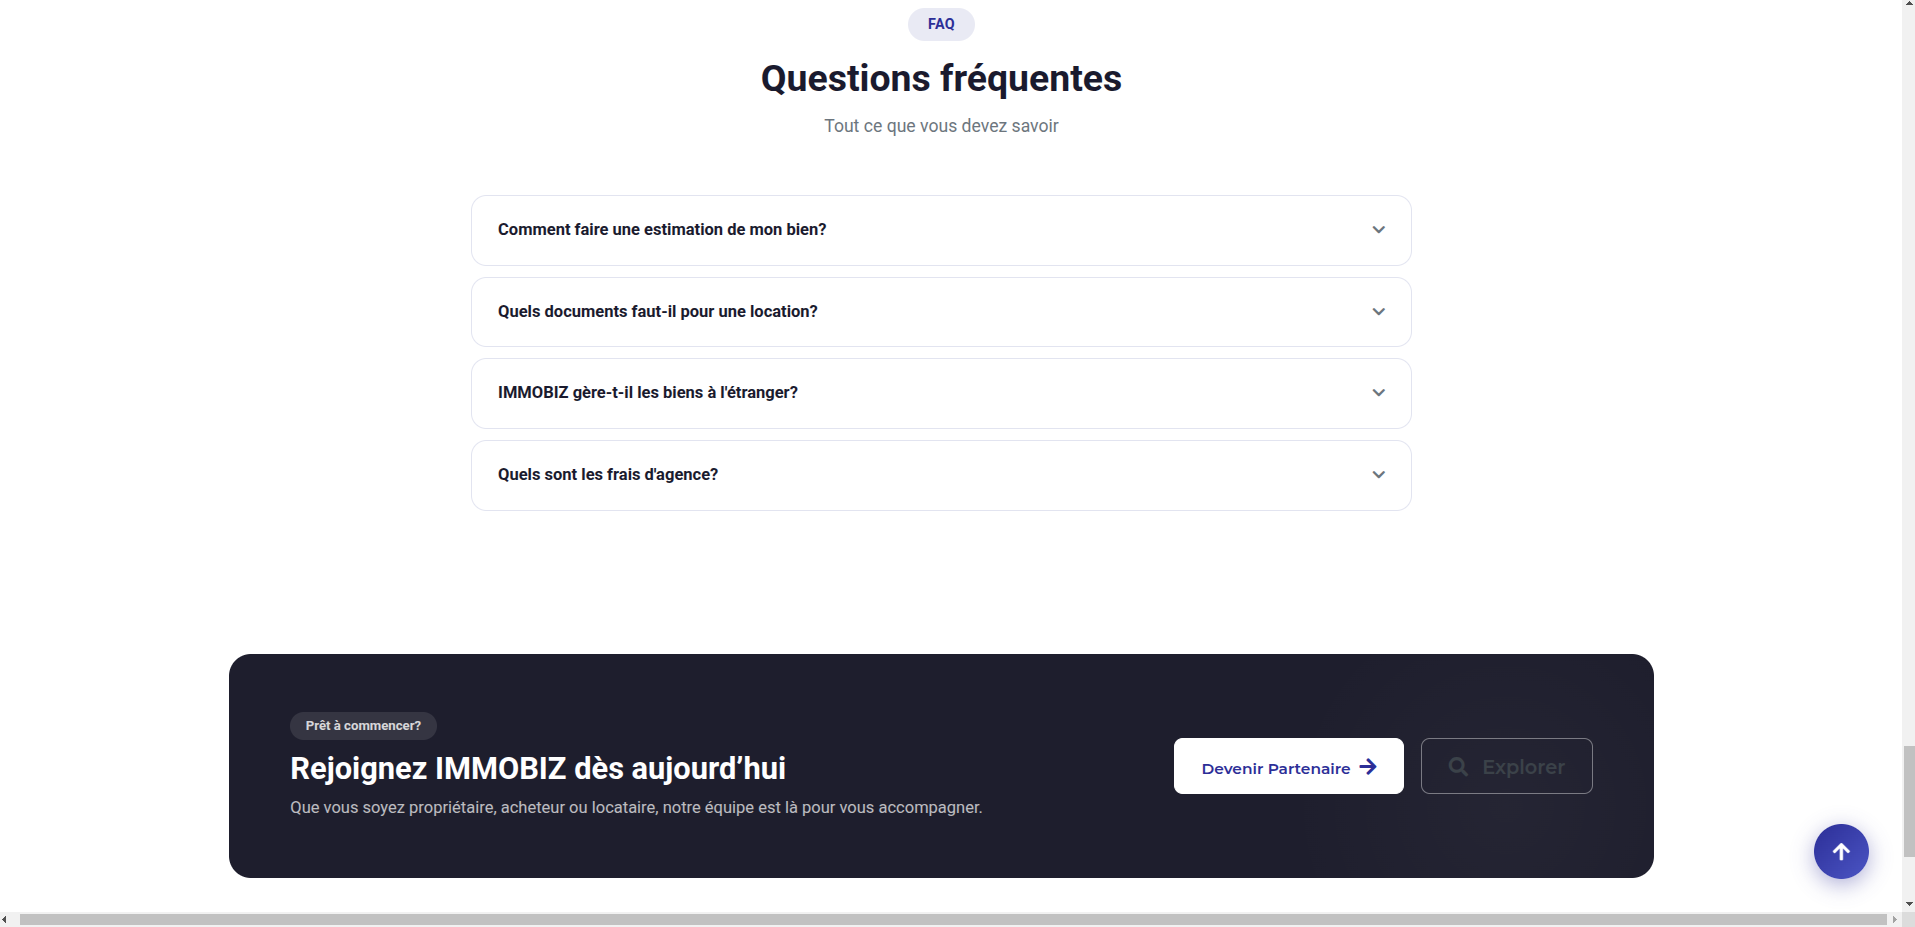
\includegraphics[width=\textwidth]{images/acueil6.png}
  
    
    
    \caption{Page d'accueil de l'application IMMOBIZ}
    \label{fig:accueil-3}
\end{figure}



\begin{figure}[H]
    \centering
  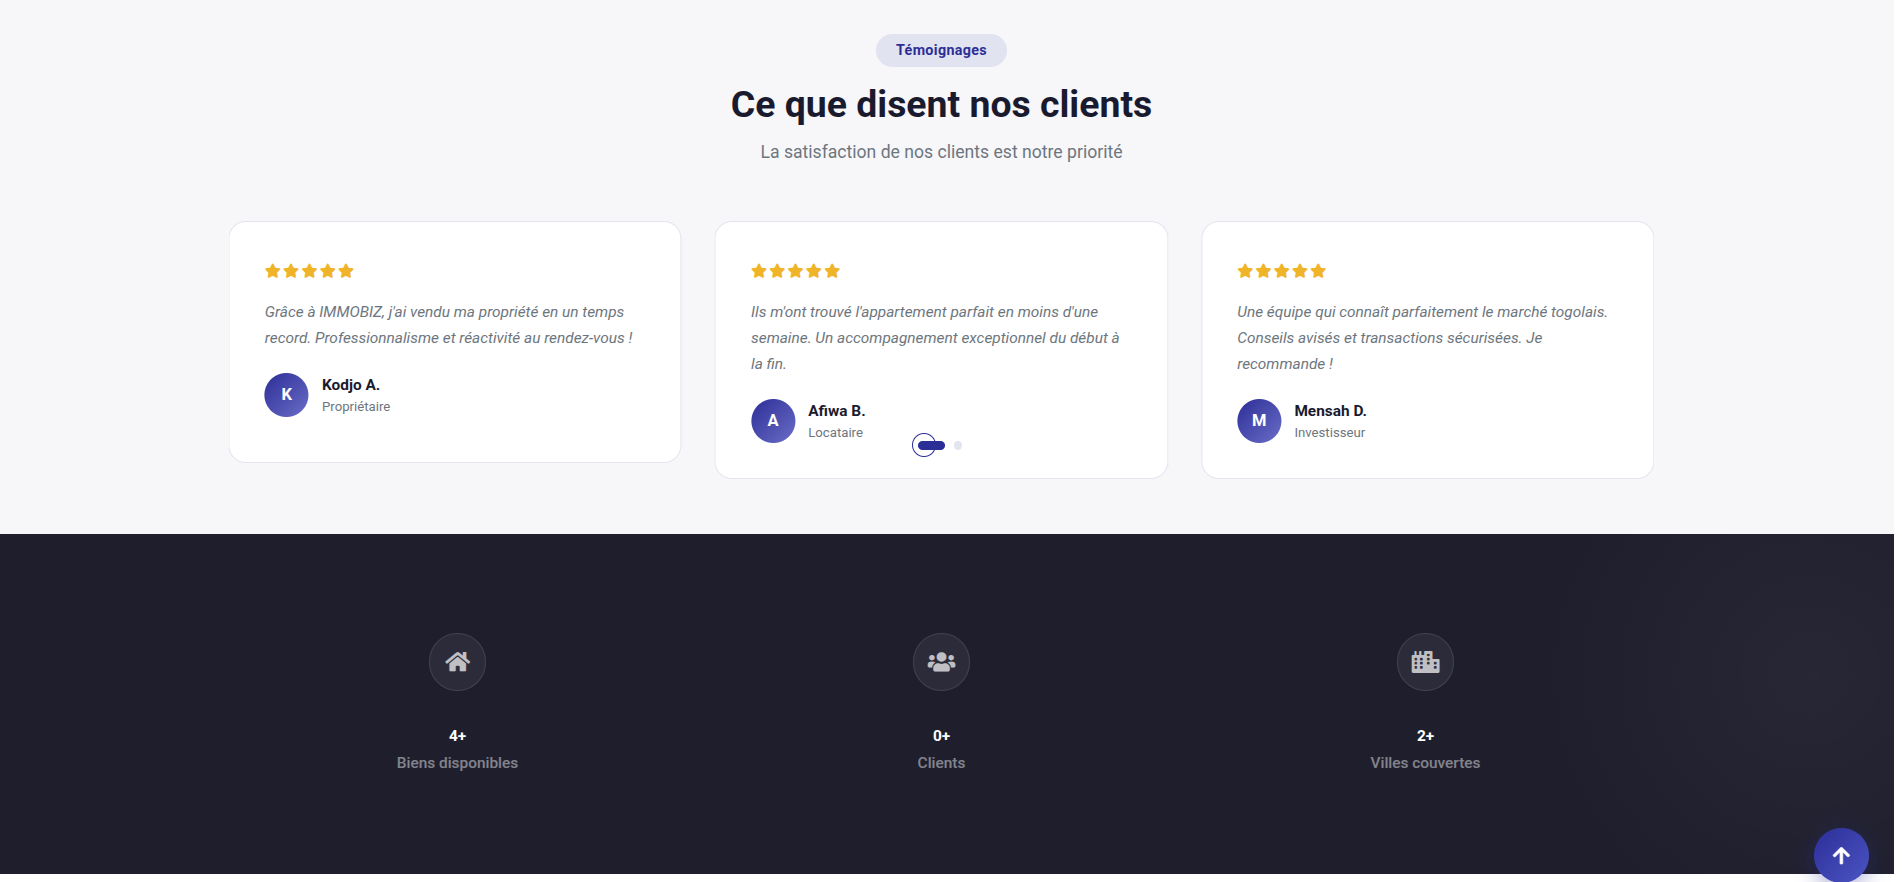
\includegraphics[width=\textwidth]{images/acueil7.png}
    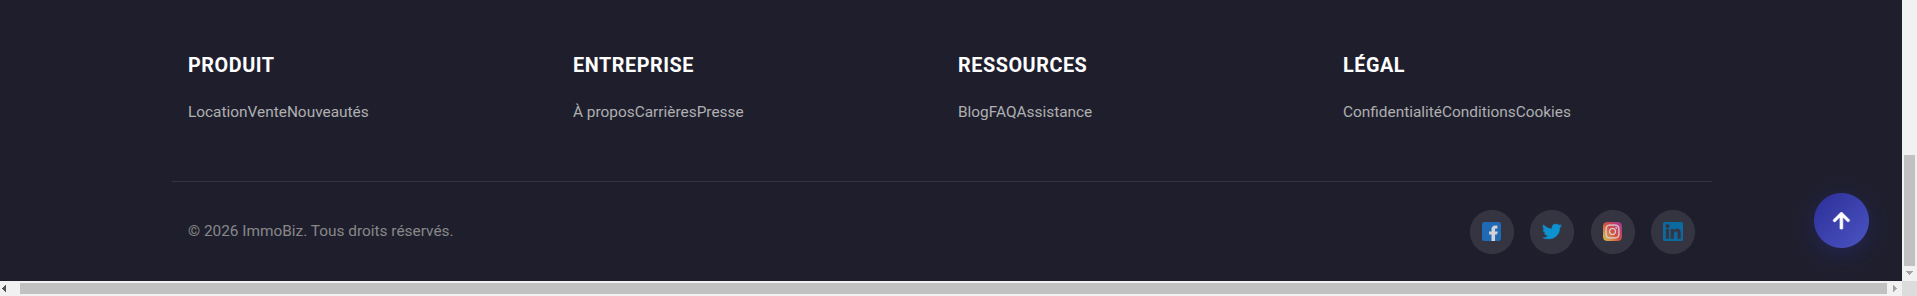
\includegraphics[width=\textwidth]{images/acueil8.png}
 \caption{Page d'accueil de l'application IMMOBIZ}
    \label{fig:accuei-4}
\end{figure}

\subsubsection{Fiche détail d'un bien}
Ci-dessous un aperçu de la page de détail d'un bien, accessible en cliquant sur le bouton « Détail » du \textbf{bien}  depuis la page d'accueil, ainsi qu'un exemple de données renseignées pour une demande de visite.

\begin{figure}[H]
    \centering
    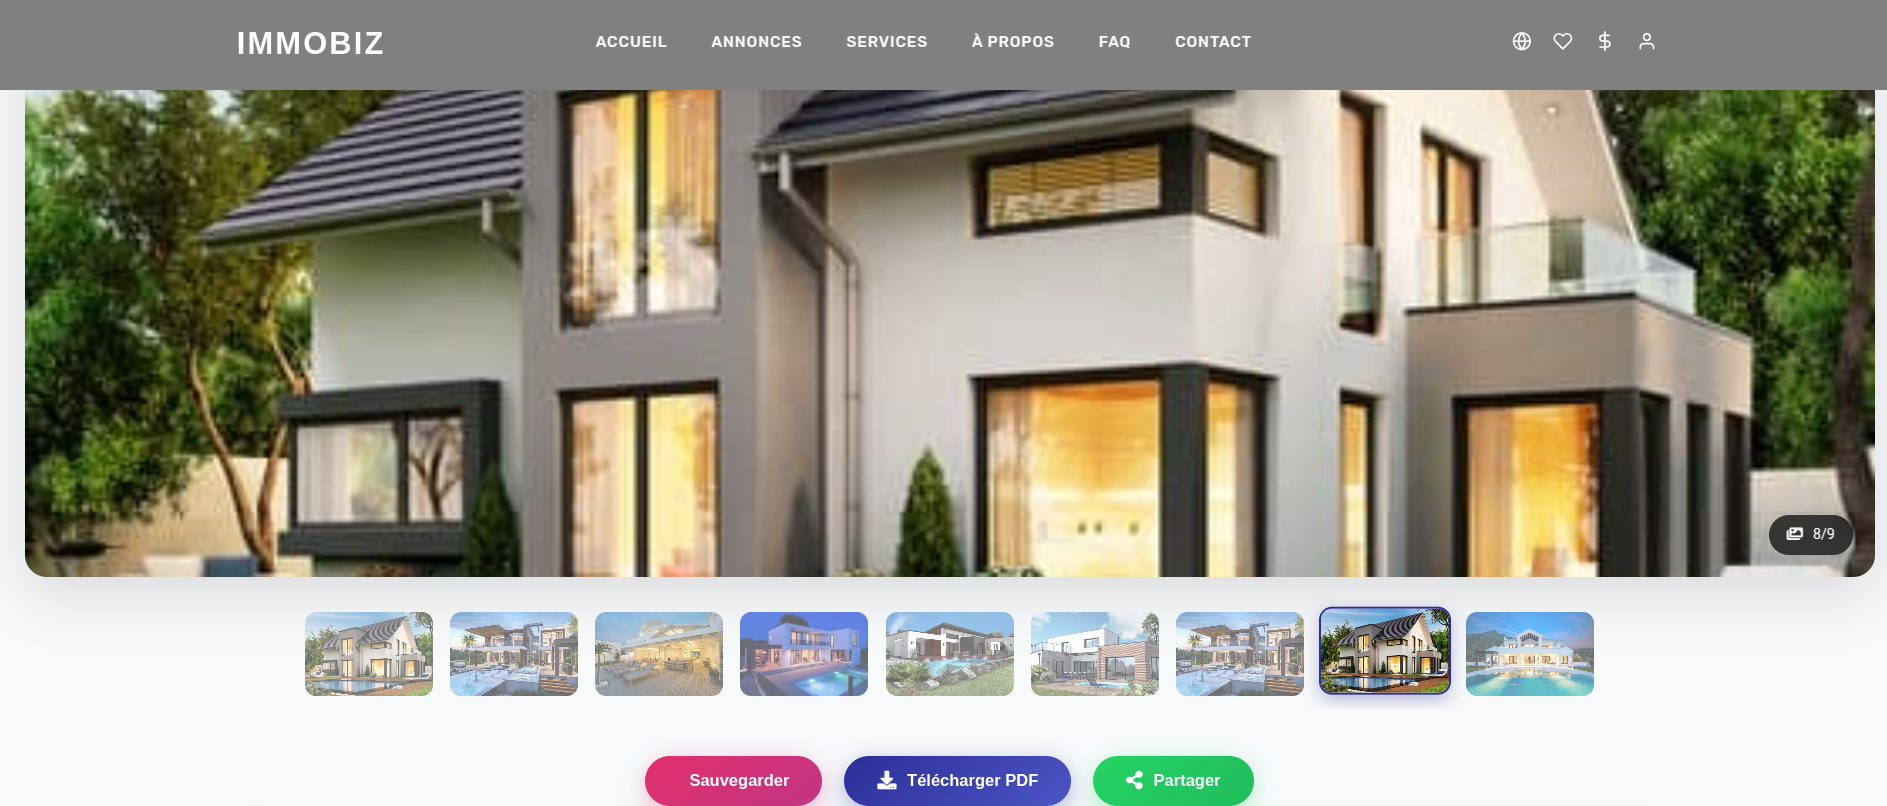
\includegraphics[width=\textwidth]{images/detail1.png}
    \caption{Fiche détail d'un bien immobilier}
    \label{fig:prospect-fiche-bien}
\end{figure}

\begin{figure}[H]
    \centering
    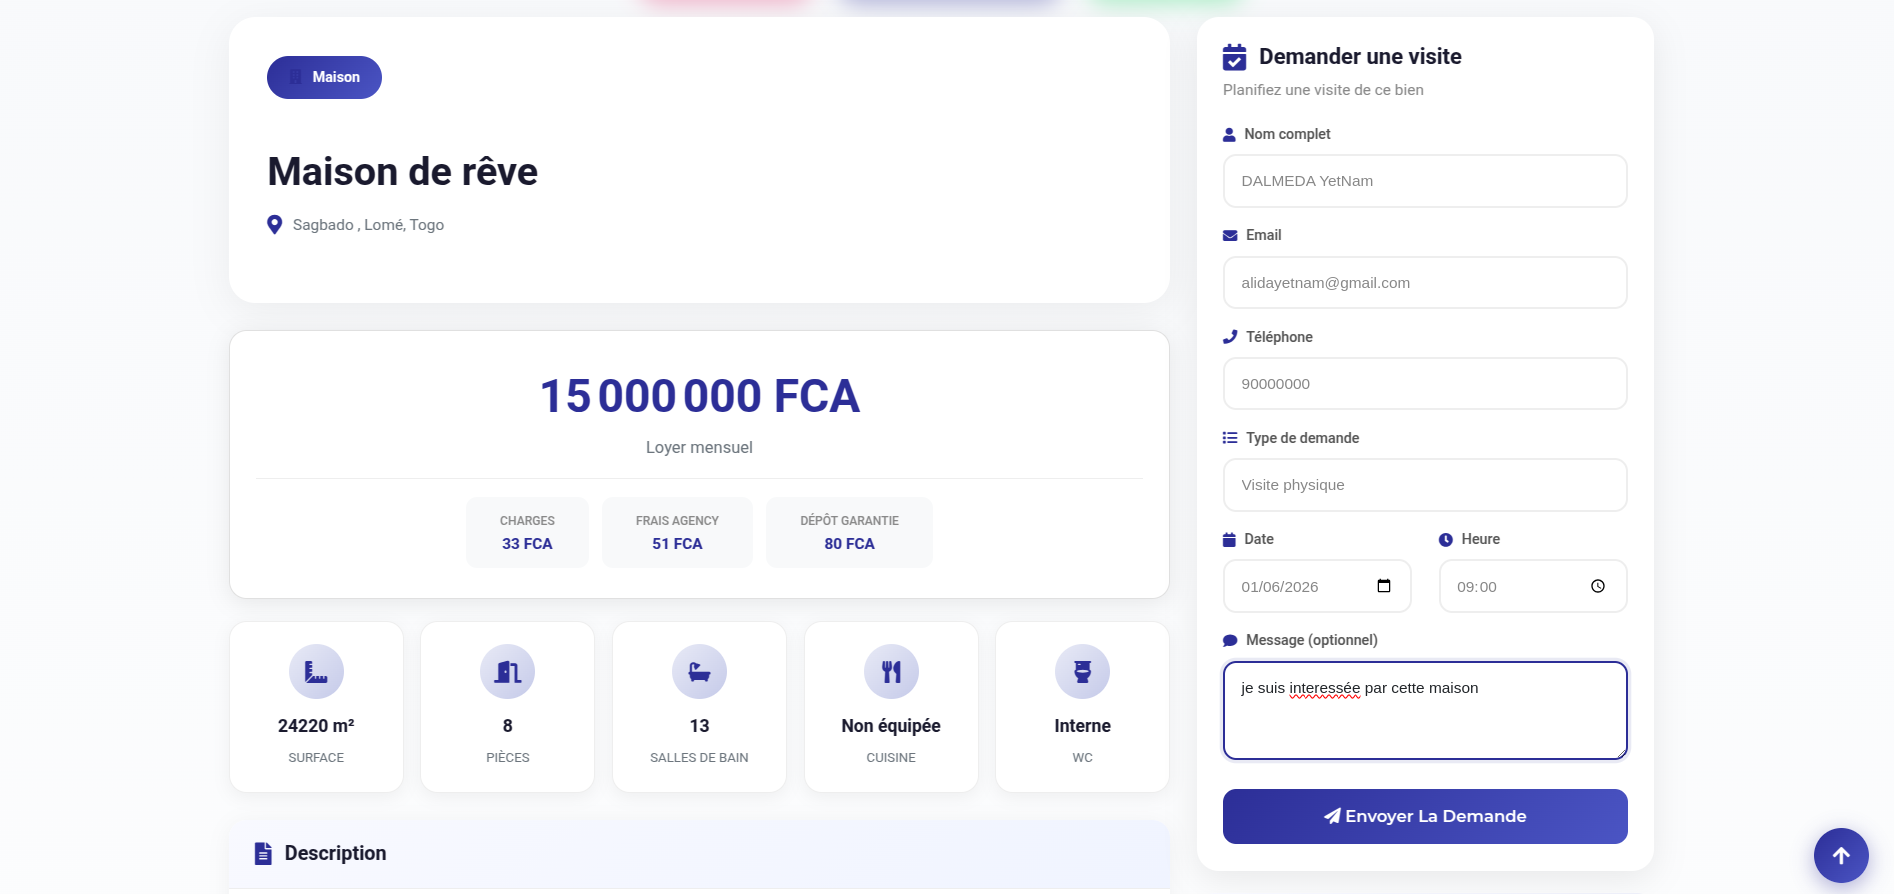
\includegraphics[width=\textwidth]{images/detail2.png}
    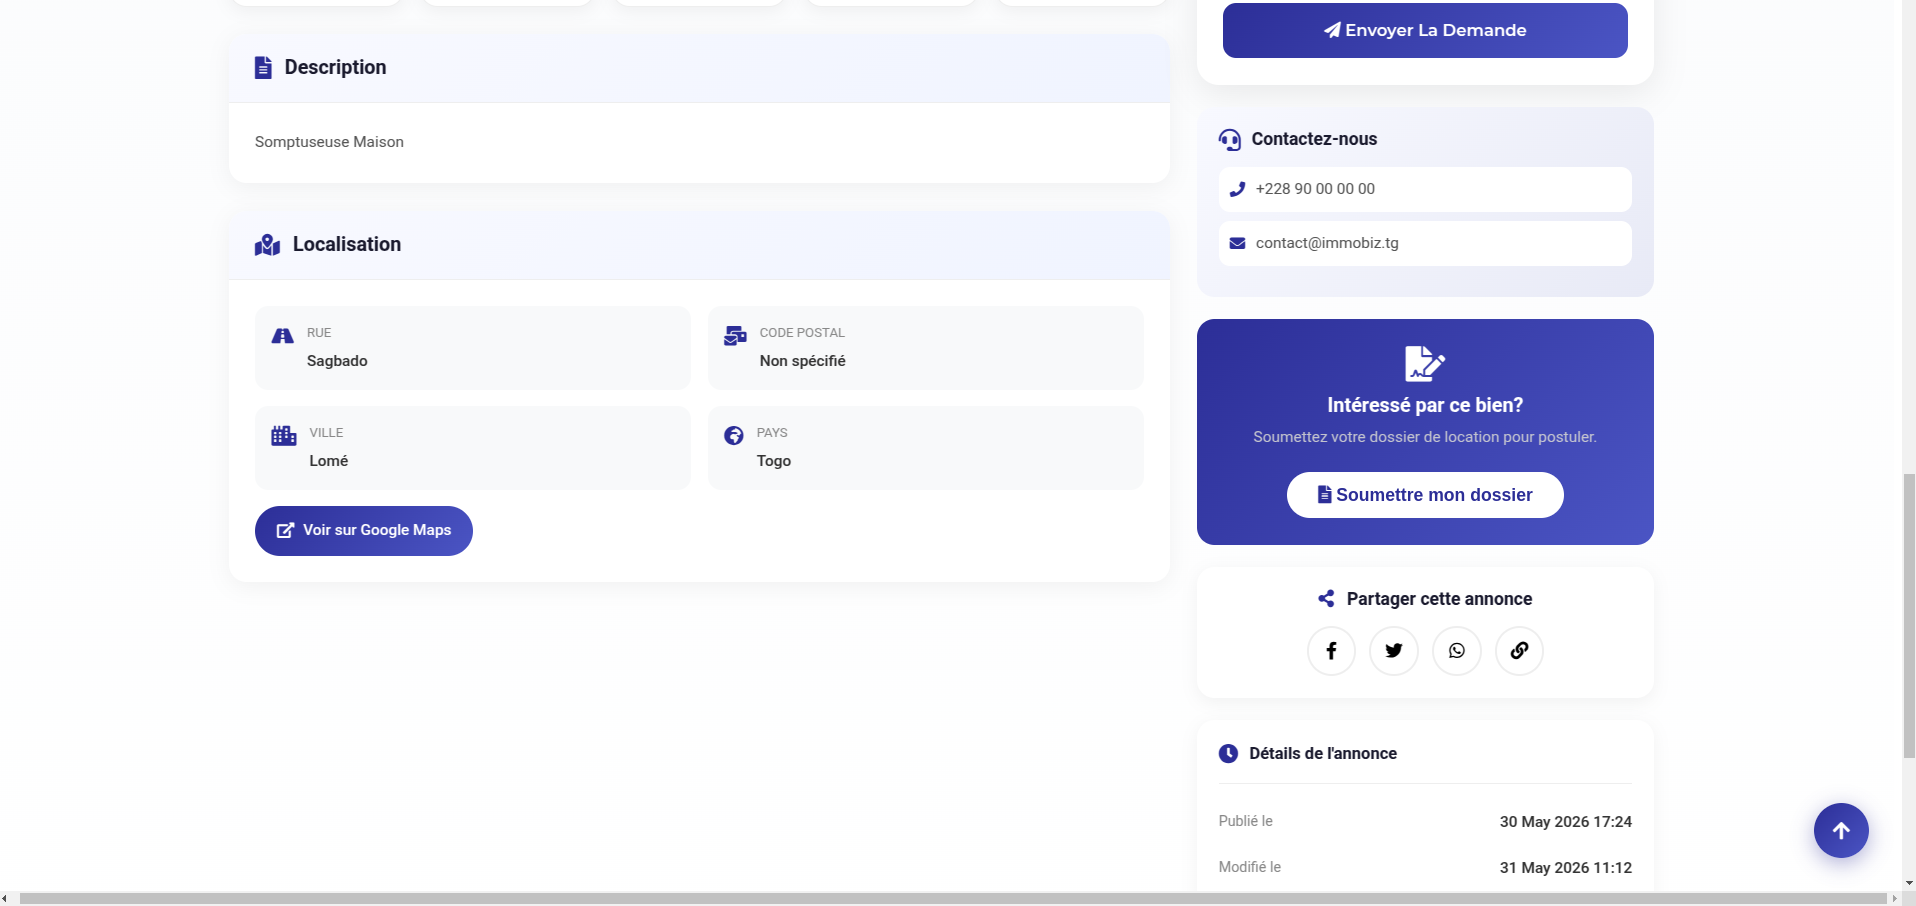
\includegraphics[width=\textwidth]{images/detail3.png}

    \caption{Fiche détail d'un bien immobilier}
    \label{fig:prospect-fiche-bien}
\end{figure}
\newpage

\subsubsection{Soumission du dossier de location}

Une fois la visite effectuée et le prospect convaincu par le bien, ce dernier peut soumettre son dossier de location directement depuis la plateforme. Ci-dessous un aperçu de la page dédiée à cette soumission.
\begin{figure}[H]
    \centering
    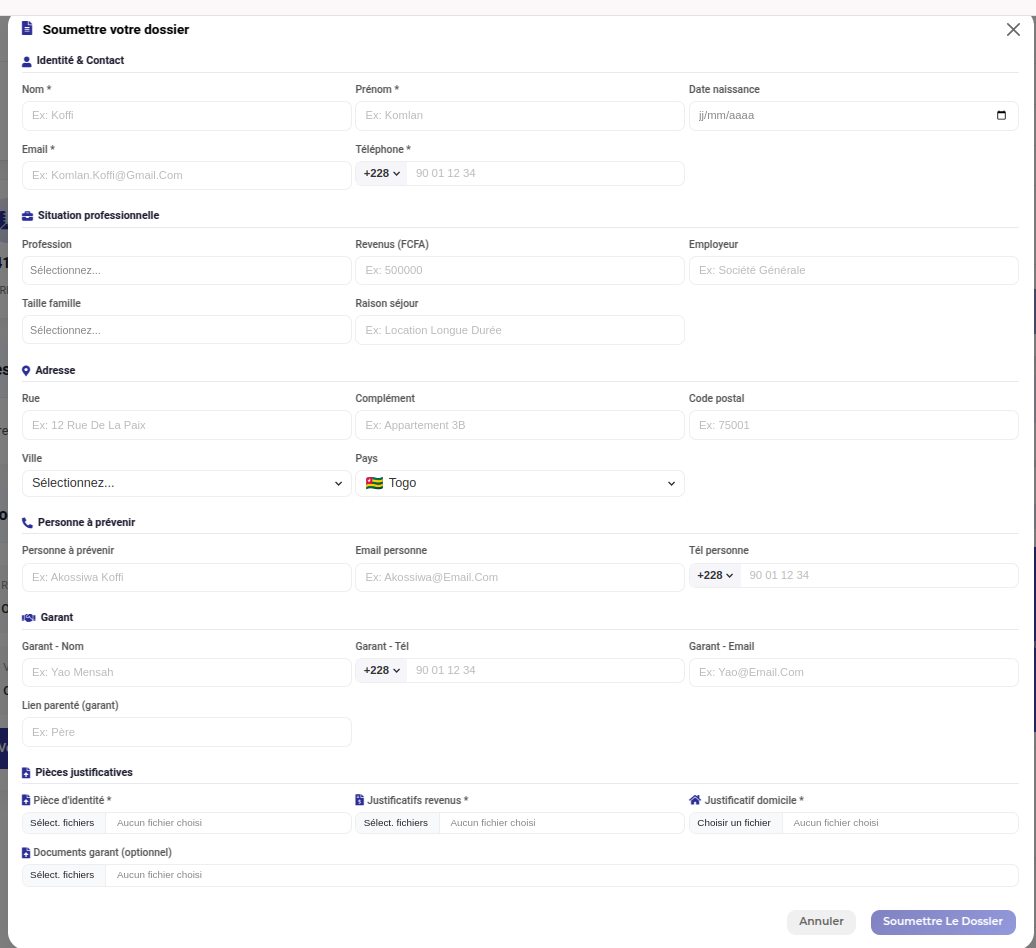
\includegraphics[width=\textwidth]{images/soumission-dossier.png}
    
    \caption{Soumission du dossier de location}
    \label{fig:prospect-dossier-location}
\end{figure}

\newpage
\subsection{Interface Prospect}
Le prospect désigne un utilisateur non authentifié ne disposant pas encore d'un compte sur la plateforme \motcle{IMMOBIZ}.
Il peut consulter la liste des biens disponibles, accéder à la fiche détail 
d'un bien, soumettre une demande de visite et déposer un dossier de location, 
le tout sans authentification préalable.


\begin{figure}[H]
    \centering
    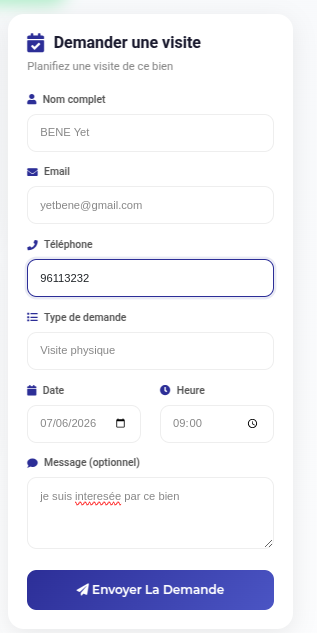
\includegraphics[width=0.50\textwidth]{images/visite-pro.png}
    \caption{Fiche de demande de visite d'un bien immobilier}
    \label{fig:prospect-fiche-bien}
\end{figure}


\subsubsection{Soumission du dossier de location}
Une fois convaincu par le bien après la visite obligatoire effectuée, le prospect soumet son dossier de location :
\begin{figure}[H]
    \centering
    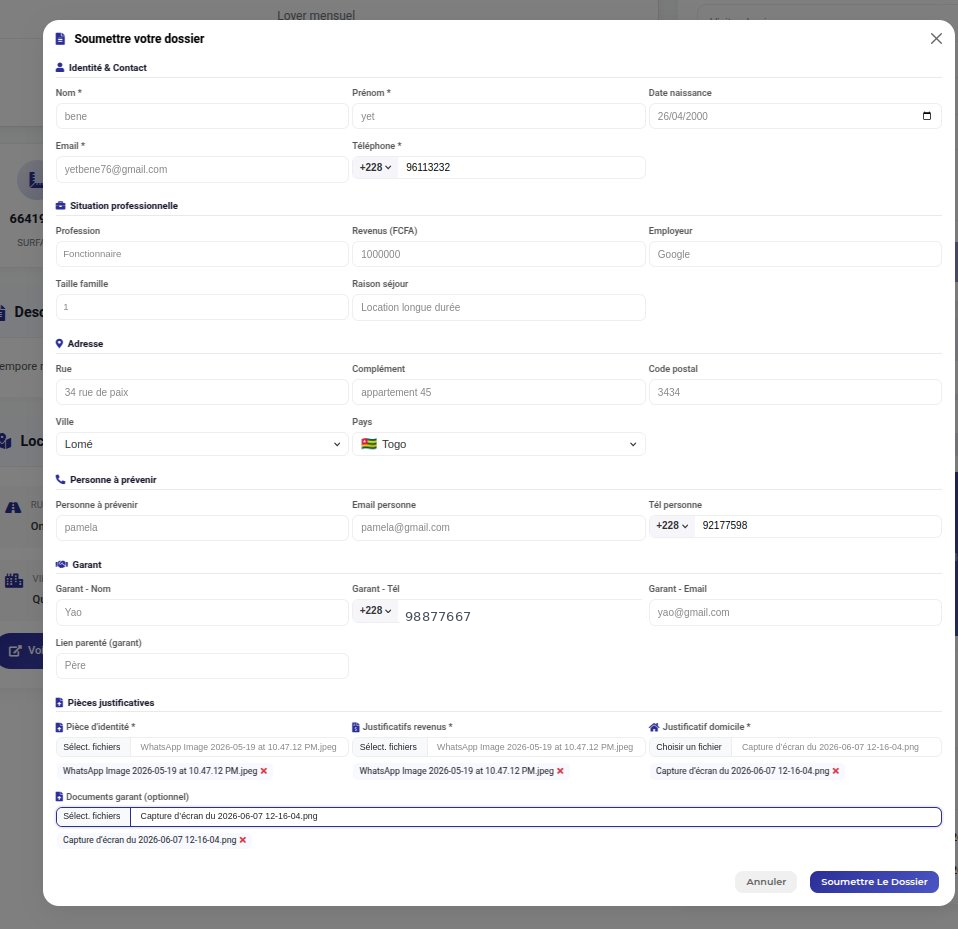
\includegraphics[width=\textwidth]{images/dossier-loc.png}
   
    \caption{Soumission du dossier de location}
    \label{fig:prospect-dossier-location}
\end{figure}









\newpage
\subsection{Authentification}


L'accès aux fonctionnalités de la plateforme \motcle{IMMOBIZ} est réservé aux utilisateurs dont la candidature a été préalablement validée. Depuis la page d'accueil, les profils \textit{Propriétaire}, \textit{Gestionnaire}, \textit{Agence immobilière} et \textit{Technicien} peuvent soumettre une demande d'adhésion à travers le bouton \textbf{« Devenir partenaire »}.


\begin{figure}[H]
    \centering
    
\includegraphics[width=\textwidth]{images/parte1.png}
    \caption{Page de connexion de l'application IMMOBIZ}
    \label{fig:login}
\end{figure}


\begin{figure}[H]
    \centering
    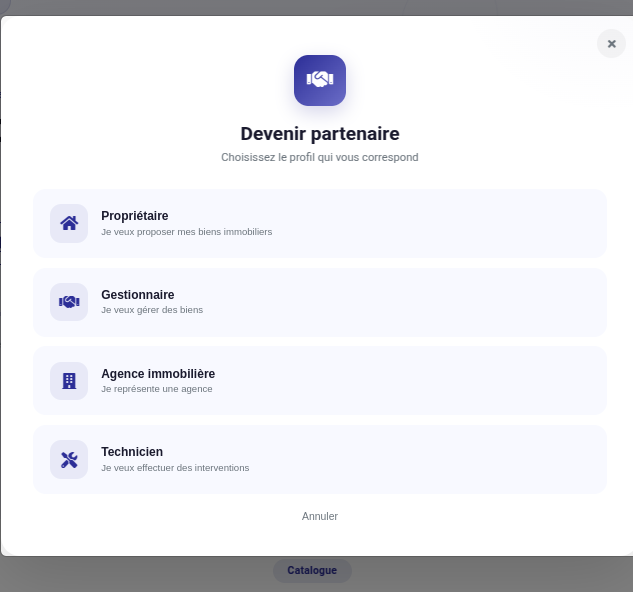
\includegraphics[width=\textwidth]{images/parte2.png}
    \caption{Page de connexion de l'application IMMOBIZ}
    \label{fig:login}
\end{figure}




Une fois la candidature soumise, un courrier électronique de confirmation est automatiquement envoyé afin d'informer le candidat de la bonne réception de sa demande. La candidature est ensuite examinée par le gérant de la plateforme qui vérifie les informations fournies et décide de son acceptation ou de son refus.

En cas d'acceptation, un compte utilisateur est créé automatiquement par le système. Un courrier électronique est alors envoyé au candidat pour l'informer de la validation de sa candidature. Ce message contient également un lien \textbf{« Créer un mot de passe »} permettant d'activer son compte et de définir ses identifiants de connexion.

Après la création de son mot de passe, l'utilisateur peut accéder à son espace personnel afin de compléter les informations complémentaires relatives à son profil et d'utiliser les fonctionnalités qui lui sont attribuées. L'ensemble de ce processus est sécurisé grâce à la bibliothèque \motcle{com.kodzotech:security-oauth2}, garantissant la confidentialité des données et la protection des accès.


La Figure ci-dessous présente l'interface de connexion permettant aux utilisateurs validés d'accéder à leur espace personnel après avoir activé leur compte.


\begin{figure}[H]
    \centering
    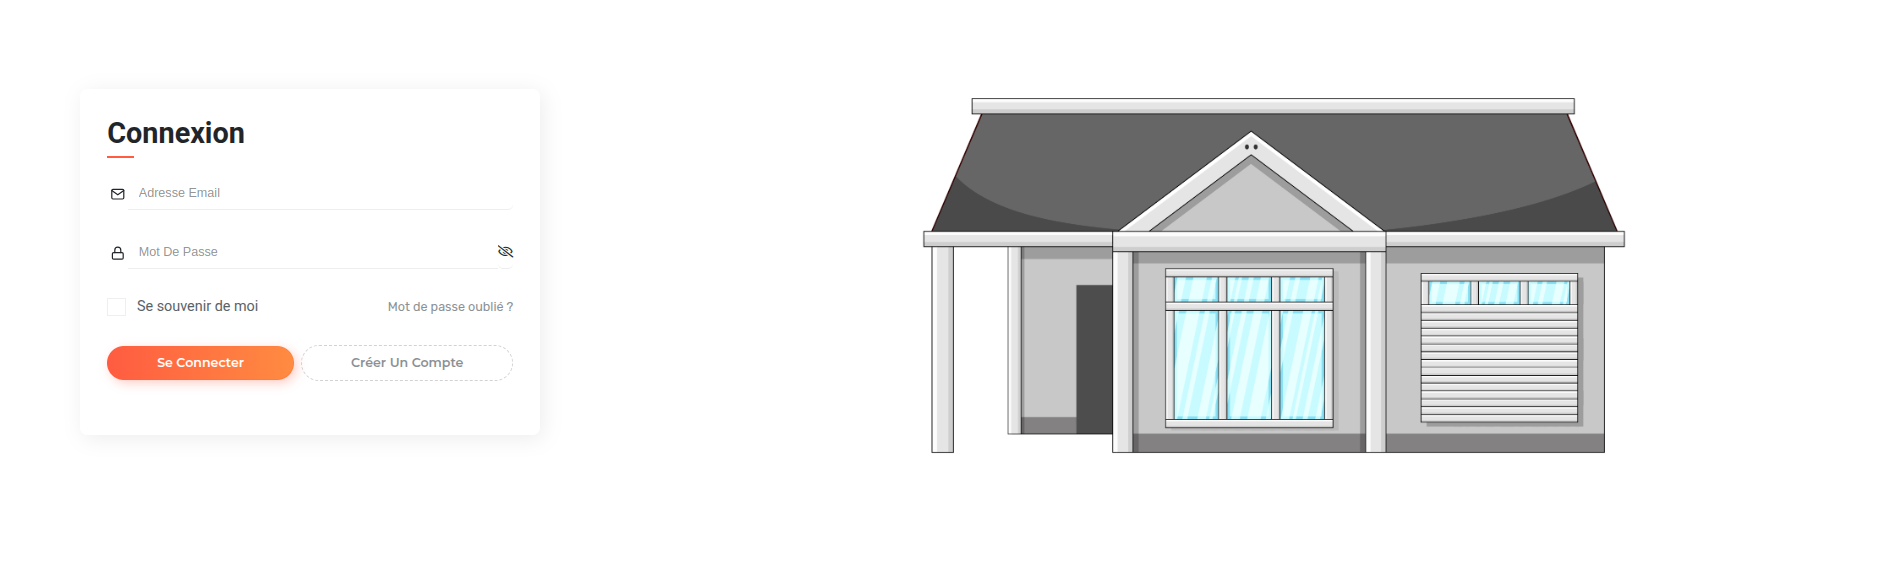
\includegraphics[width=\textwidth]{images/con.png}
    \caption{Page de connexion de l'application IMMOBIZ}
    \label{fig:login}
\end{figure}











\newpage
\subsection{Interface Propriétaire}
Le propriétaire est une personne physique disposant d'un ou plusieurs biens immobiliers qu'elle souhaite mettre en location ou proposer à la vente. Pour accéder à son espace de gestion, il doit au préalable s'authentifier via la page de connexion en renseignant ses identifiants. Une fois authentifié, il est redirigé vers son tableau de bord personnel.\\
\\
La figure ci-dessus illustre l'interface du propriétaire une fois connecté. Le menu latéral gauche lui donne accès à l'ensemble des fonctionnalités de gestion : Tableau de bord, Mes Biens, Demandes de Location, Locataires, Contrats, Visites, États des Lieux, Documents, Messages, Paiements, Notifications et Mon Profil, centralisant ainsi toutes les actions en un seul espace.


\begin{figure}[H]
    \centering
    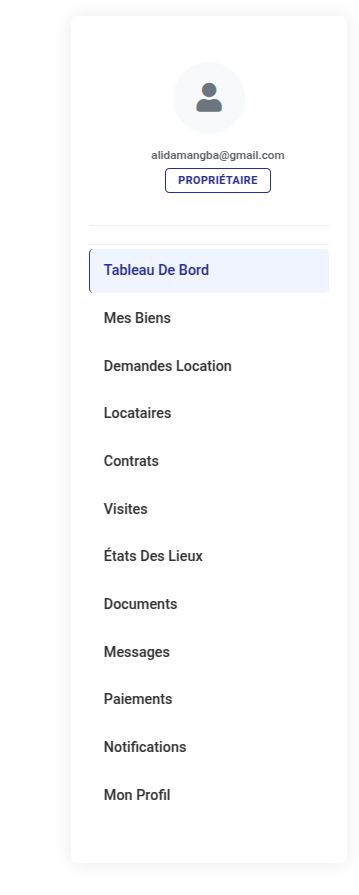
\includegraphics[width=0.50\textwidth]{images/pro-sid.png}
    \caption{Bar latéral du propriétaire}
    
\end{figure}






\subsubsection{Calcul du score }

Dès la soumission d'une demande de location, le système \motcle{IMMOBIZ} calcule automatiquement un score de solvabilité sur 100 points, réparti selon sept critères :
\begin{itemize}
\item \textbf{Complétude du dossier (15 pts)} : évalue la présence des informations personnelles (nom, email, téléphone, profession, employeur, revenus, taille de la famille) ainsi que les documents joints (pièce d'identité, justificatif de revenus, justificatif de domicile).
\item \textbf{Stabilité des revenus (25 pts)} : prend en compte l'ancienneté professionnelle du candidat. Une ancienneté supérieure à 3 ans rapporte le maximum de points, entre 1 et 3 ans un score intermédiaire, et moins d'un an un score minimal.

\item \textbf{Ratio revenus/loyer (25 pts)} : mesure la capacité financière du candidat en comparant ses revenus mensuels au loyer du bien. Un ratio supérieur ou égal à 4 permet d'obtenir le maximum de points.

\item \textbf{Qualité du garant (15 pts)} : valorise la présence d'un garant. Des points supplémentaires sont attribués si le garant renseigne son numéro de téléphone et son adresse email.

\item \textbf{Âge du demandeur (10 pts)} : les candidats âgés de 25 à 55 ans obtiennent le score maximum sur ce critère, les autres majeurs un score partiel.

\item \textbf{Raison du séjour (5 pts)} : attribue des points si le candidat a renseigné la raison de sa demande de location.

\item \textbf{Avis précédents (5 pts)} : points attribués par défaut en attendant l'implémentation future de l'historique des candidatures.
\end{itemize}
\textbf{Cas particulier : Bien non visité}
Si le prospect n'a pas effectué de visite du bien avant de soumettre son dossier, le score est automatiquement fixé à \textbf{15 points}, indépendamment des autres critères, traduisant un niveau d'engagement jugé insuffisant.
\end{tcolorbox}\\
\\
Ce système de scoring offre au gestionnaire un indicateur objectif et immédiat pour orienter son analyse, sans pour autant se substituer à son jugement final lors de la décision d'acceptation ou de rejet du dossier.



\subsubsection{Traitement d'un dossier de location}

La section "Demandes de Location" affiche sous forme de tableau les dossiers reçus, avec pour chaque prospect ses informations de contact, le bien concerné, le score automatiquement calculé et le statut de sa demande. Le propriétaire peut ainsi consulter, analyser et traiter chaque dossier directement depuis cette interface.



\begin{figure}[H]
    \centering
    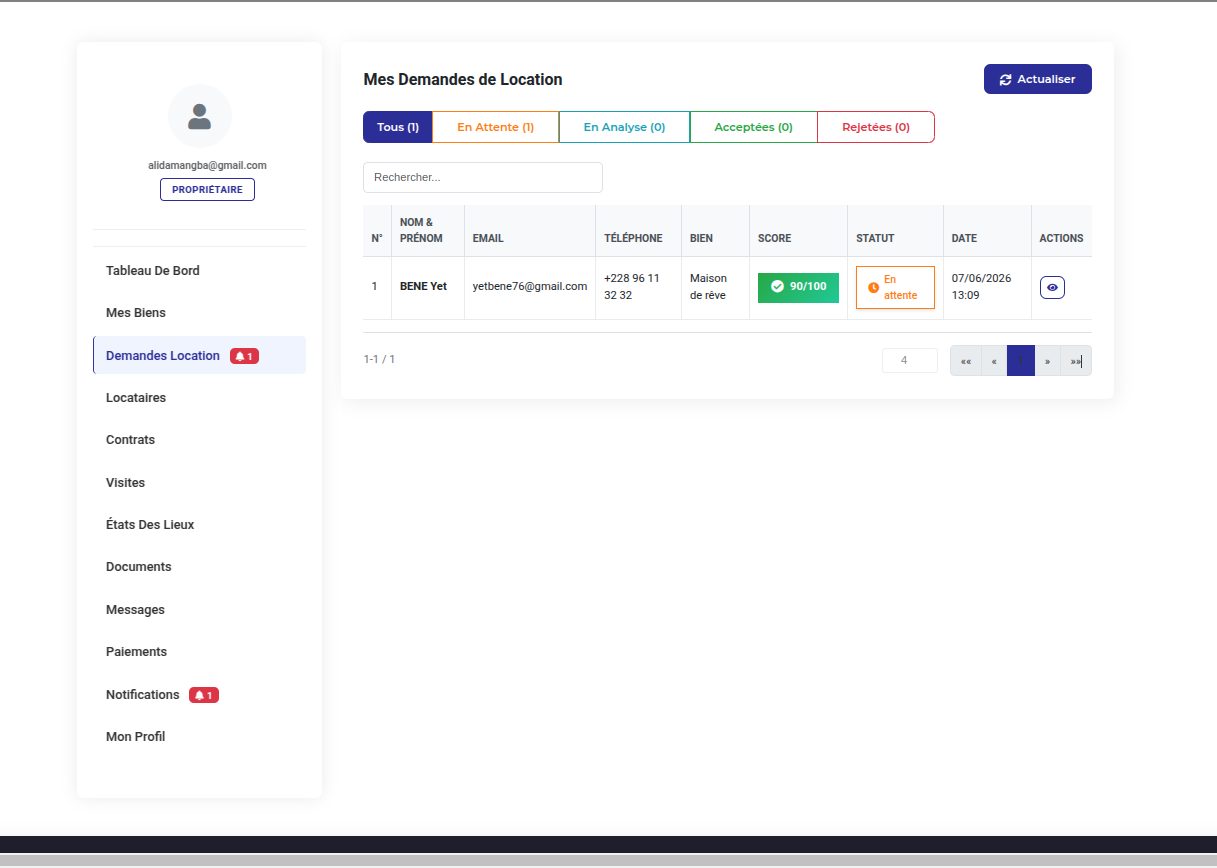
\includegraphics[width=\textwidth]{images/dossier-locavi.png}
    \caption{La liste des dossiers de location}
\end{figure}





\begin{figure}[H]
    \centering
     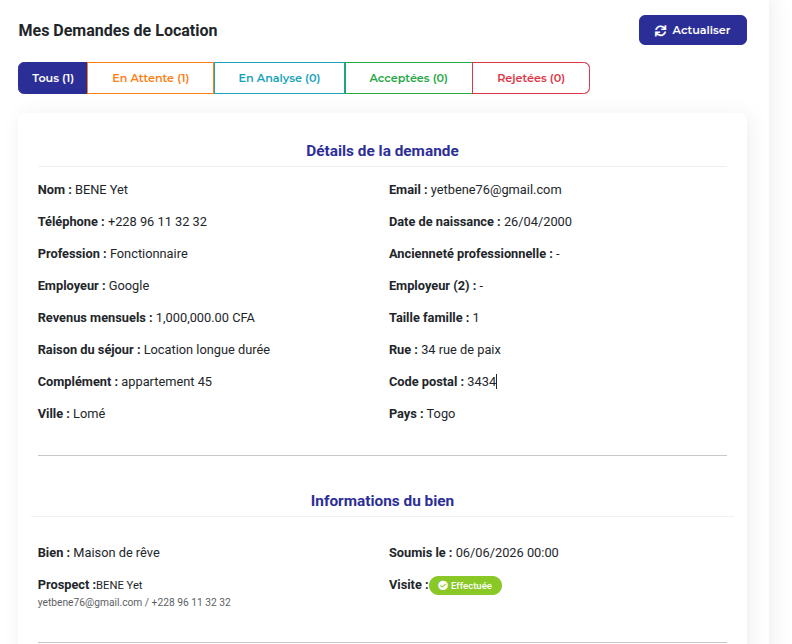
\includegraphics[width=0.75\textwidth]{images/dossi1.png}
      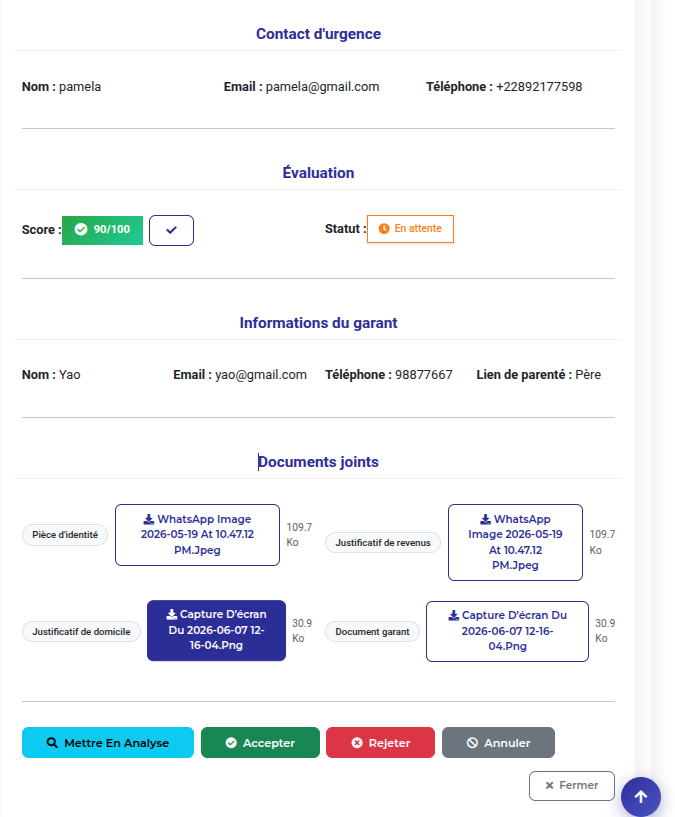
\includegraphics[width=0.75\textwidth]{images/dossi3.png}
    \caption{La page de détail de la demande}
\end{figure}

\newpage





\begin{figure}[H]
    \centering
    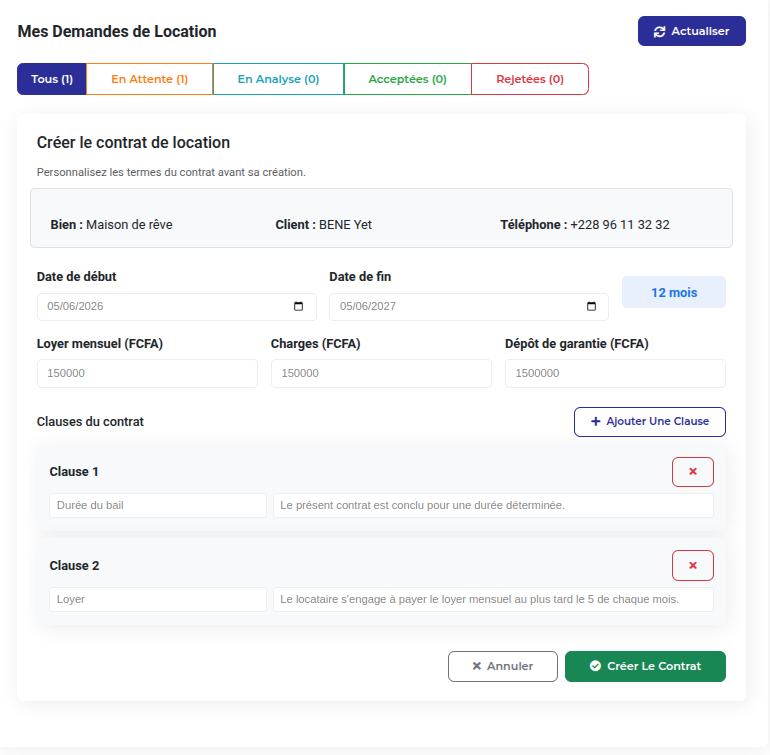
\includegraphics[width=\textwidth]{images/contr.png}

    \caption{L'édition du contrat}
    \label{fig:prospect-fiche-bien}
\end{figure}

Une fois le dossier analysé et jugé satisfaisant, le propriétaire clique sur 
le bouton \textbf{"Accepter"}. Cette action ne valide pas immédiatement la 
demande, mais redirige automatiquement le propriétaire vers l'interface 
d'édition du contrat de location, préalablement généré par défaut par la 
plateforme. Le propriétaire peut ainsi personnaliser le contrat  selon ses besoins, 
en ajustant les clauses, les dates, le montant du loyer ou toute autre 
clause qu'il juge nécessaire.

Ce n'est qu'une fois le contrat finalisé et après avoir cliqué sur le bouton 
\textbf{"Créer le contrat"} que la validation devient effective : le compte 
locataire est alors automatiquement créé au nom du prospect sur la plateforme, 
et un e-mail lui est envoyé l'invitant à définir son mot de passe afin 
d'accéder à son espace personnel.


Au-delà de la gestion des demandes de location, l'interface propriétaire 
offre un ensemble de fonctionnalités complémentaires accessibles depuis 
le menu latéral. Les figures suivantes présentent brièvement les 
différentes sections disponibles.



\begin{figure}[H]
    \centering
    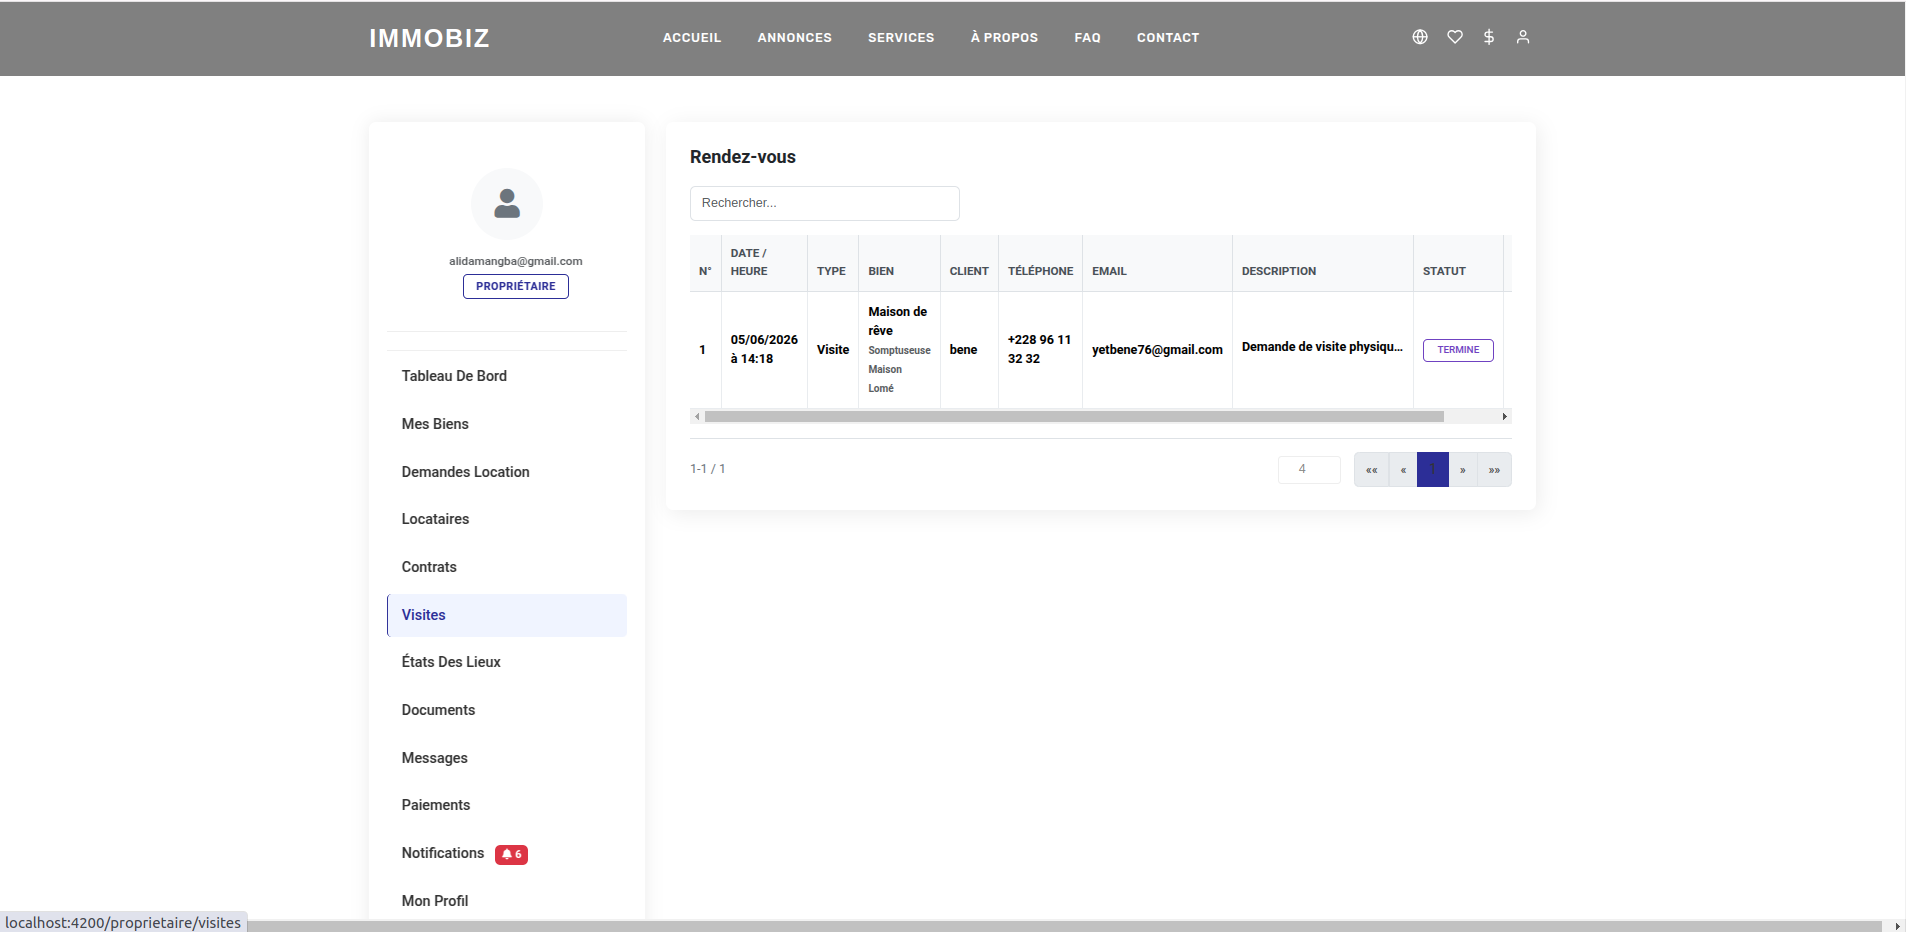
\includegraphics[width=\textwidth]{images/proprietaire-locataire.png}
    \caption{Liste des visites }
    \label{fig:prospect-fiche-bien}
\end{figure}

\begin{figure}[H]
    \centering
    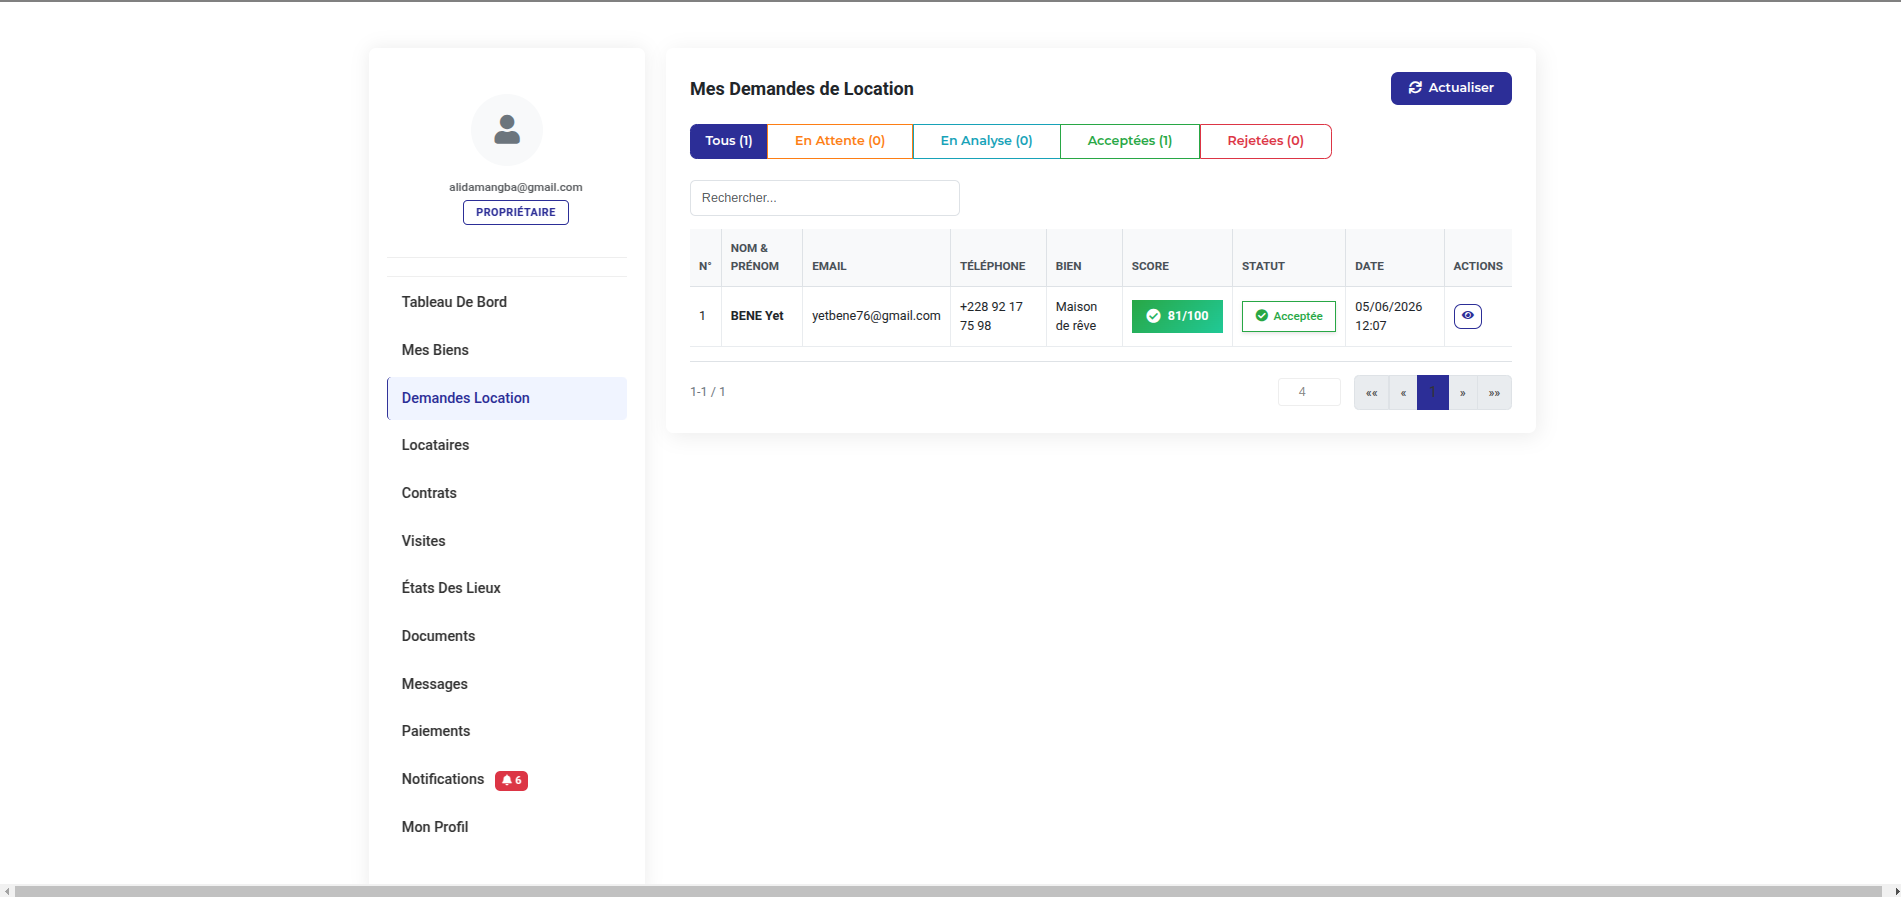
\includegraphics[width=\textwidth]{images/propretaire-dossierlocation.png}
    \caption{Liste  de tous les dossiers de location}
    \label{fig:prospect-fiche-bien}
\end{figure}

\begin{figure}[H]
    \centering
    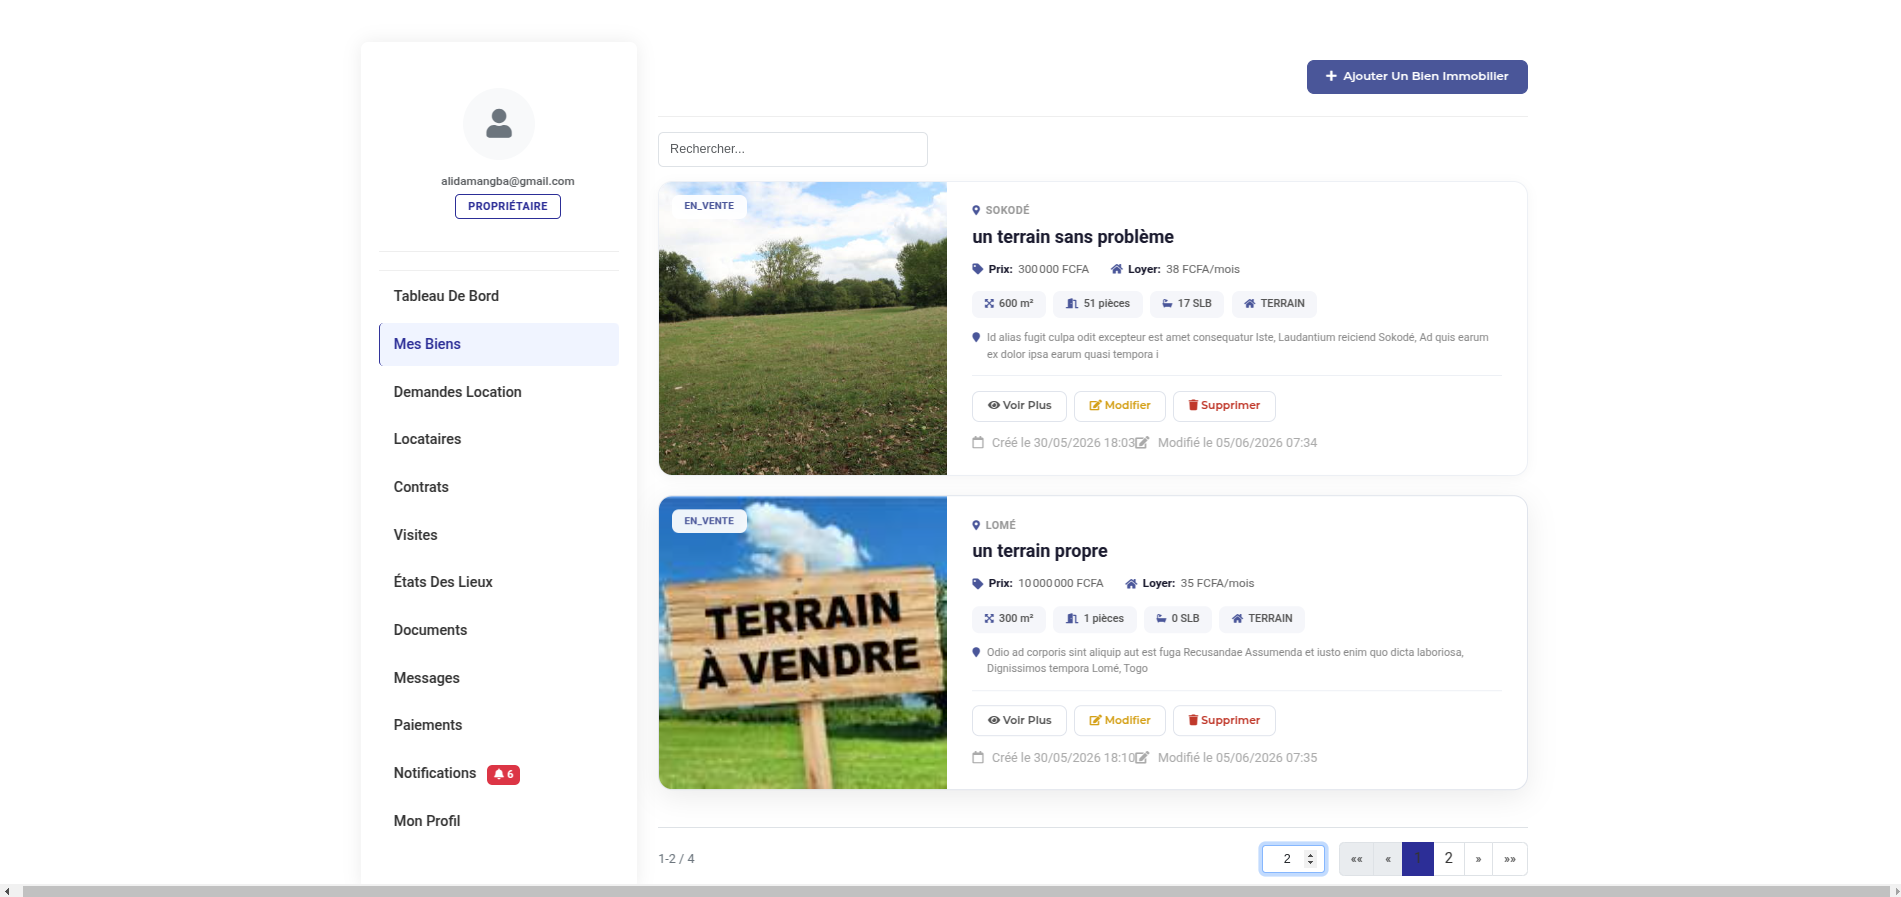
\includegraphics[width=\textwidth]{images/proretaire-bien.png}
    \caption{Liste des biens du  propriétaire}
    \label{fig:prospect-fiche-bien}
\end{figure}
è


\begin{figure}[H]
    \centering
    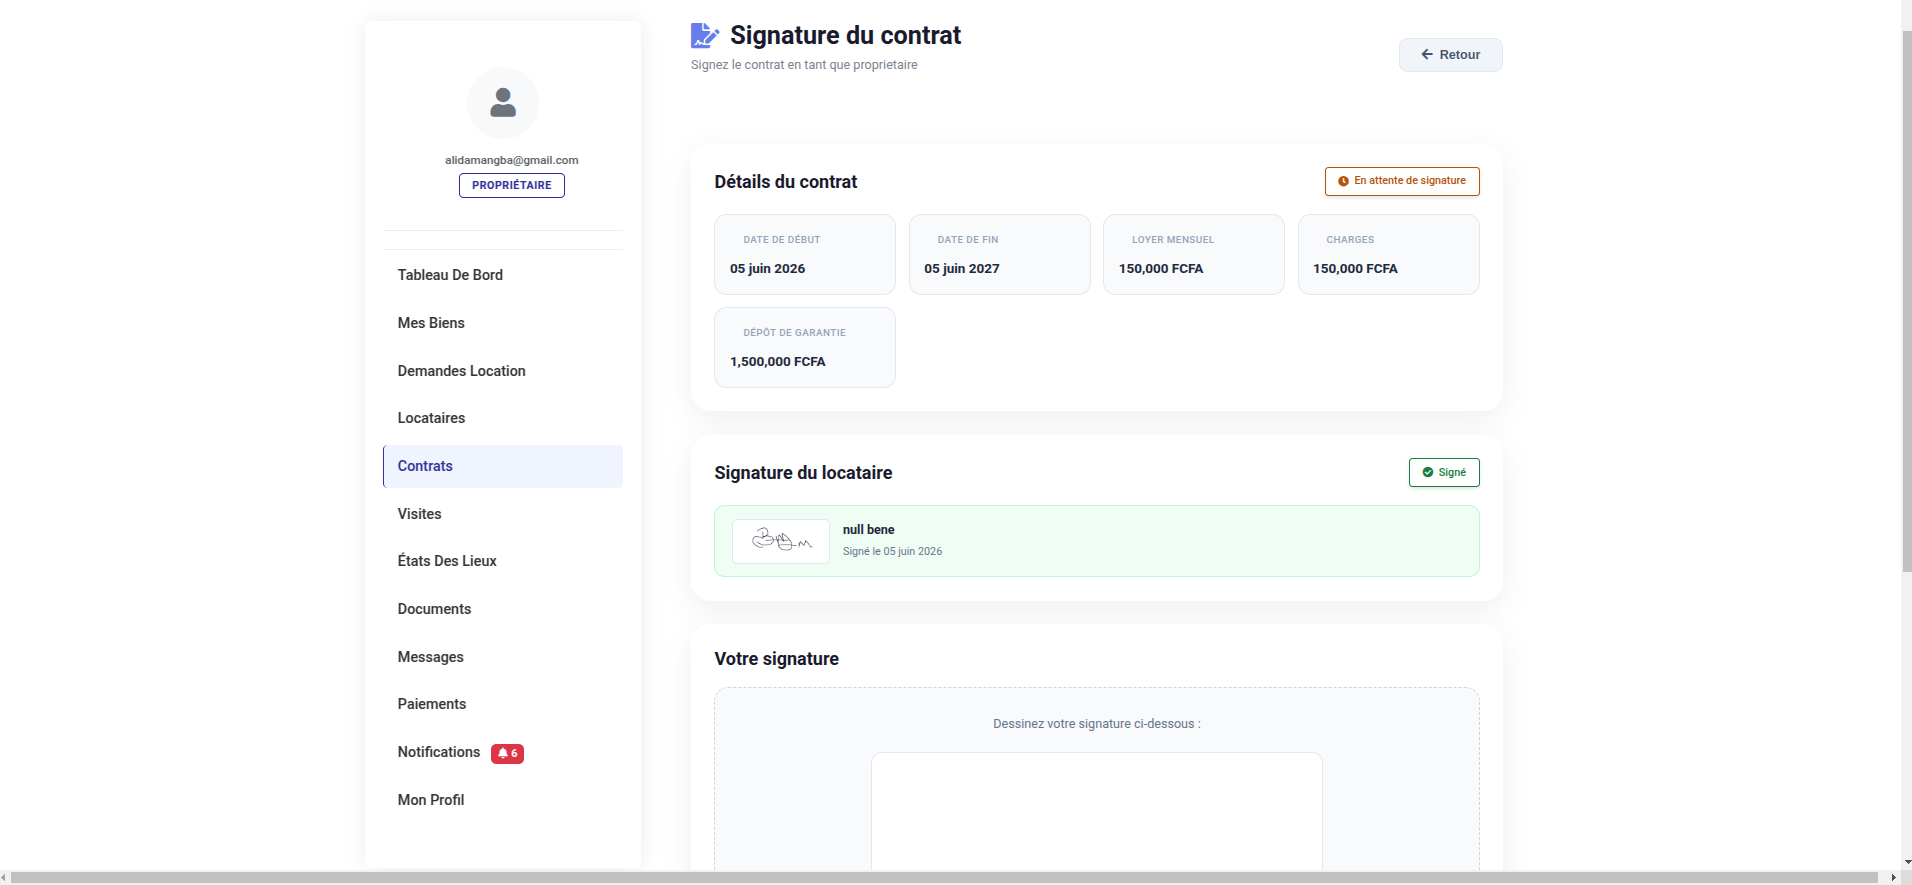
\includegraphics[width=\textwidth]{images/signer1.png}
       
    \caption{Contrat de location}
    \label{fig:prospect-fiche-bien}
\end{figure}


\begin{figure}[H]
    \centering
    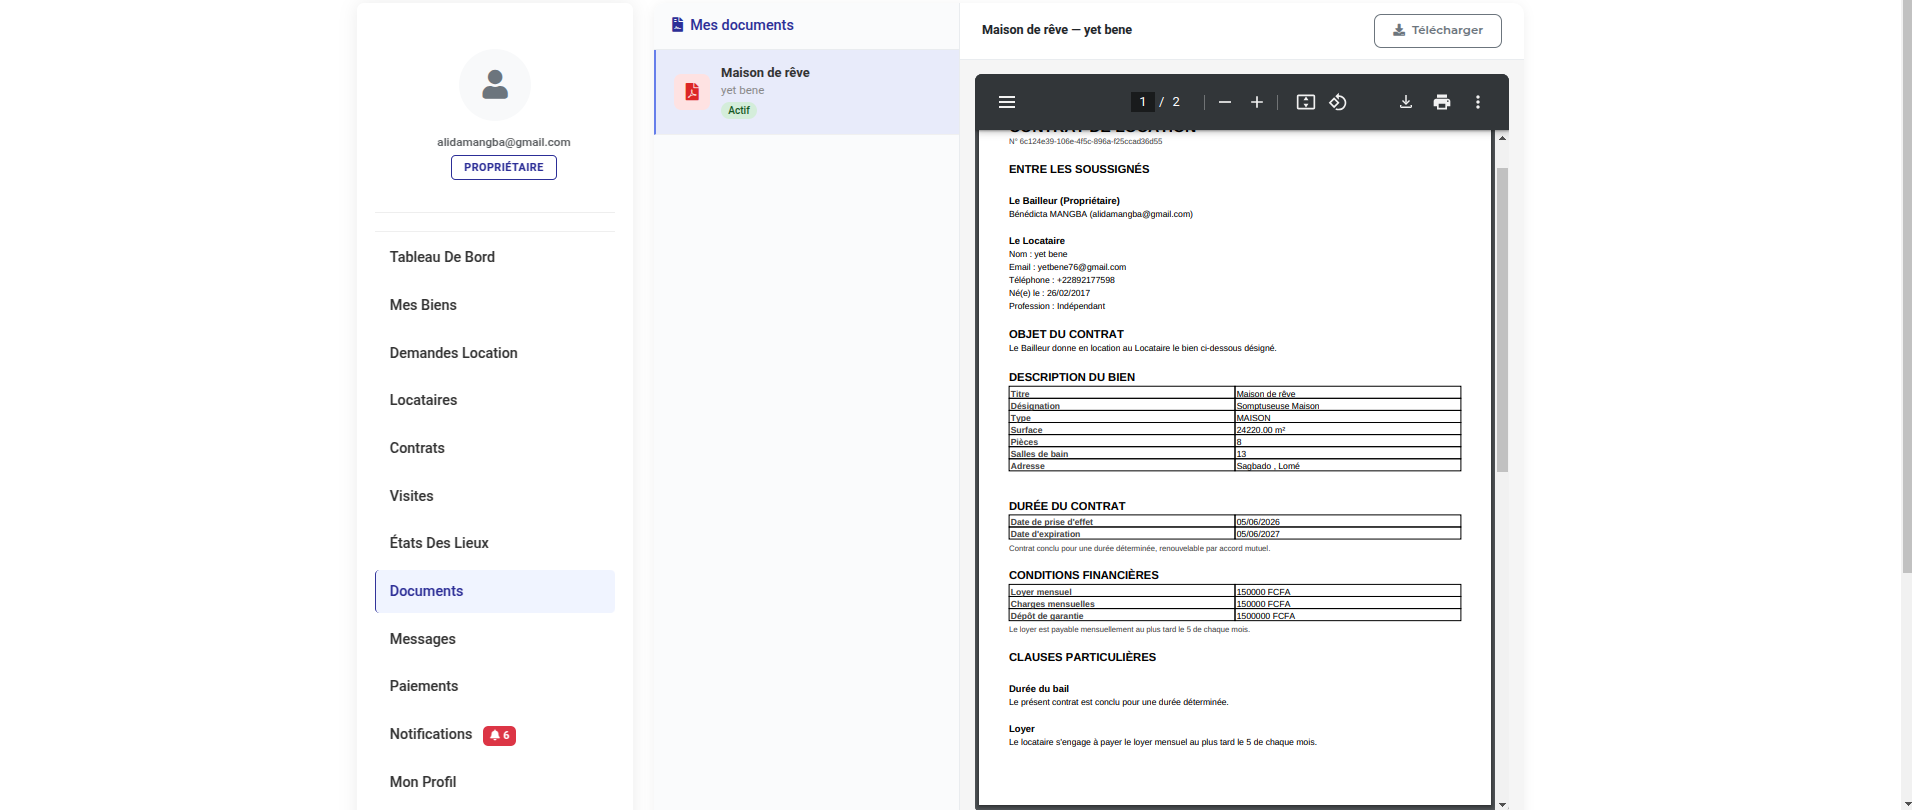
\includegraphics[width=1\textwidth]{images/contrat1.png}
        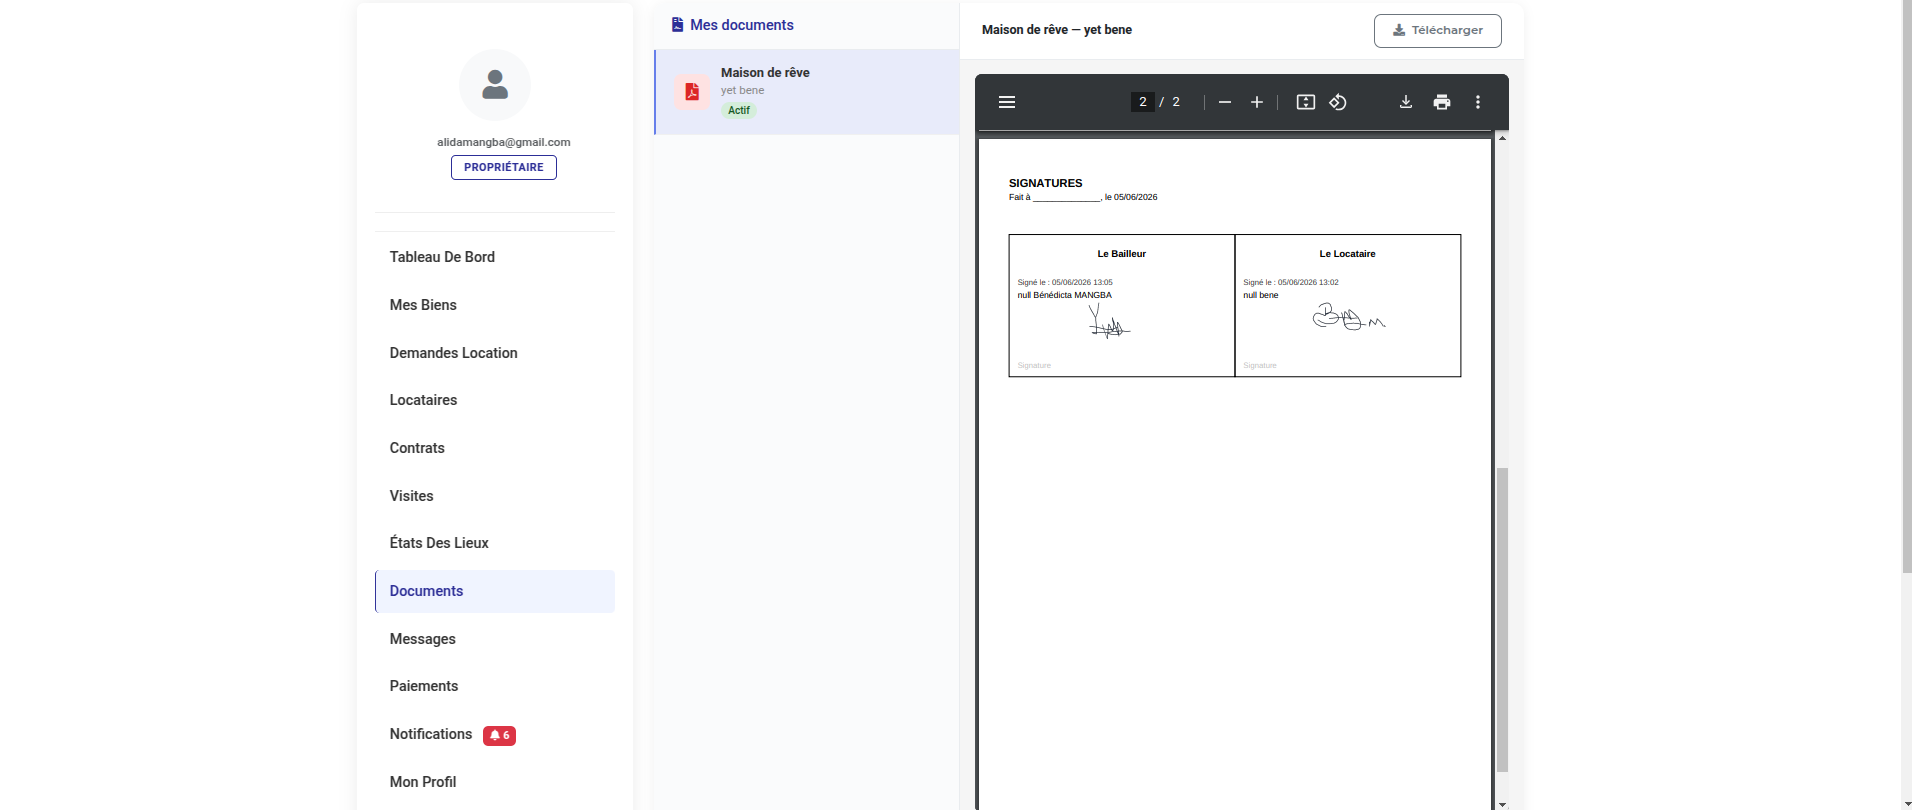
\includegraphics[width=1\textwidth]{images/contrat2.png}
    \caption{Le contrat}
    \label{fig:prospect-fiche-bien}
\end{figure}


\begin{figure}[H]
    \centering
        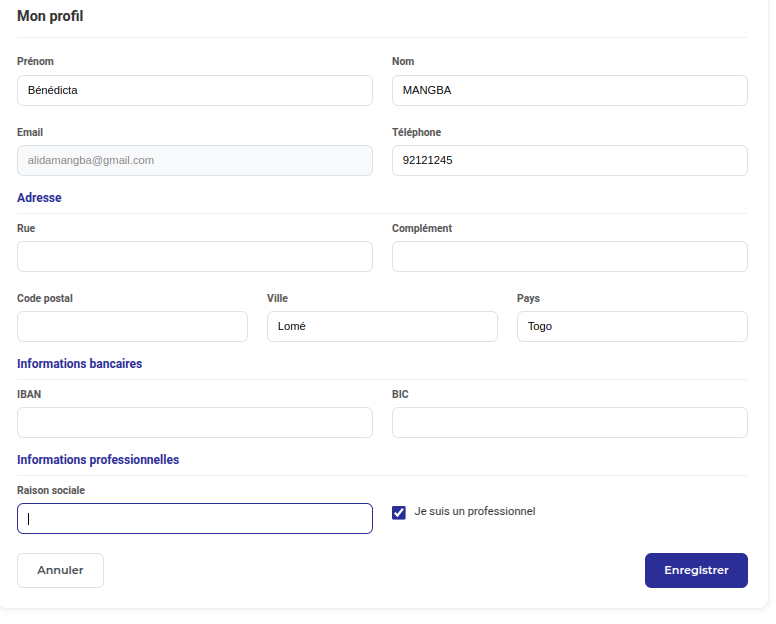
\includegraphics[width=\textwidth]{images/profil-pro.png}
    \caption{Profil Propriétaire}

\end{figure}

\begin{figure}[H]
    \centering
        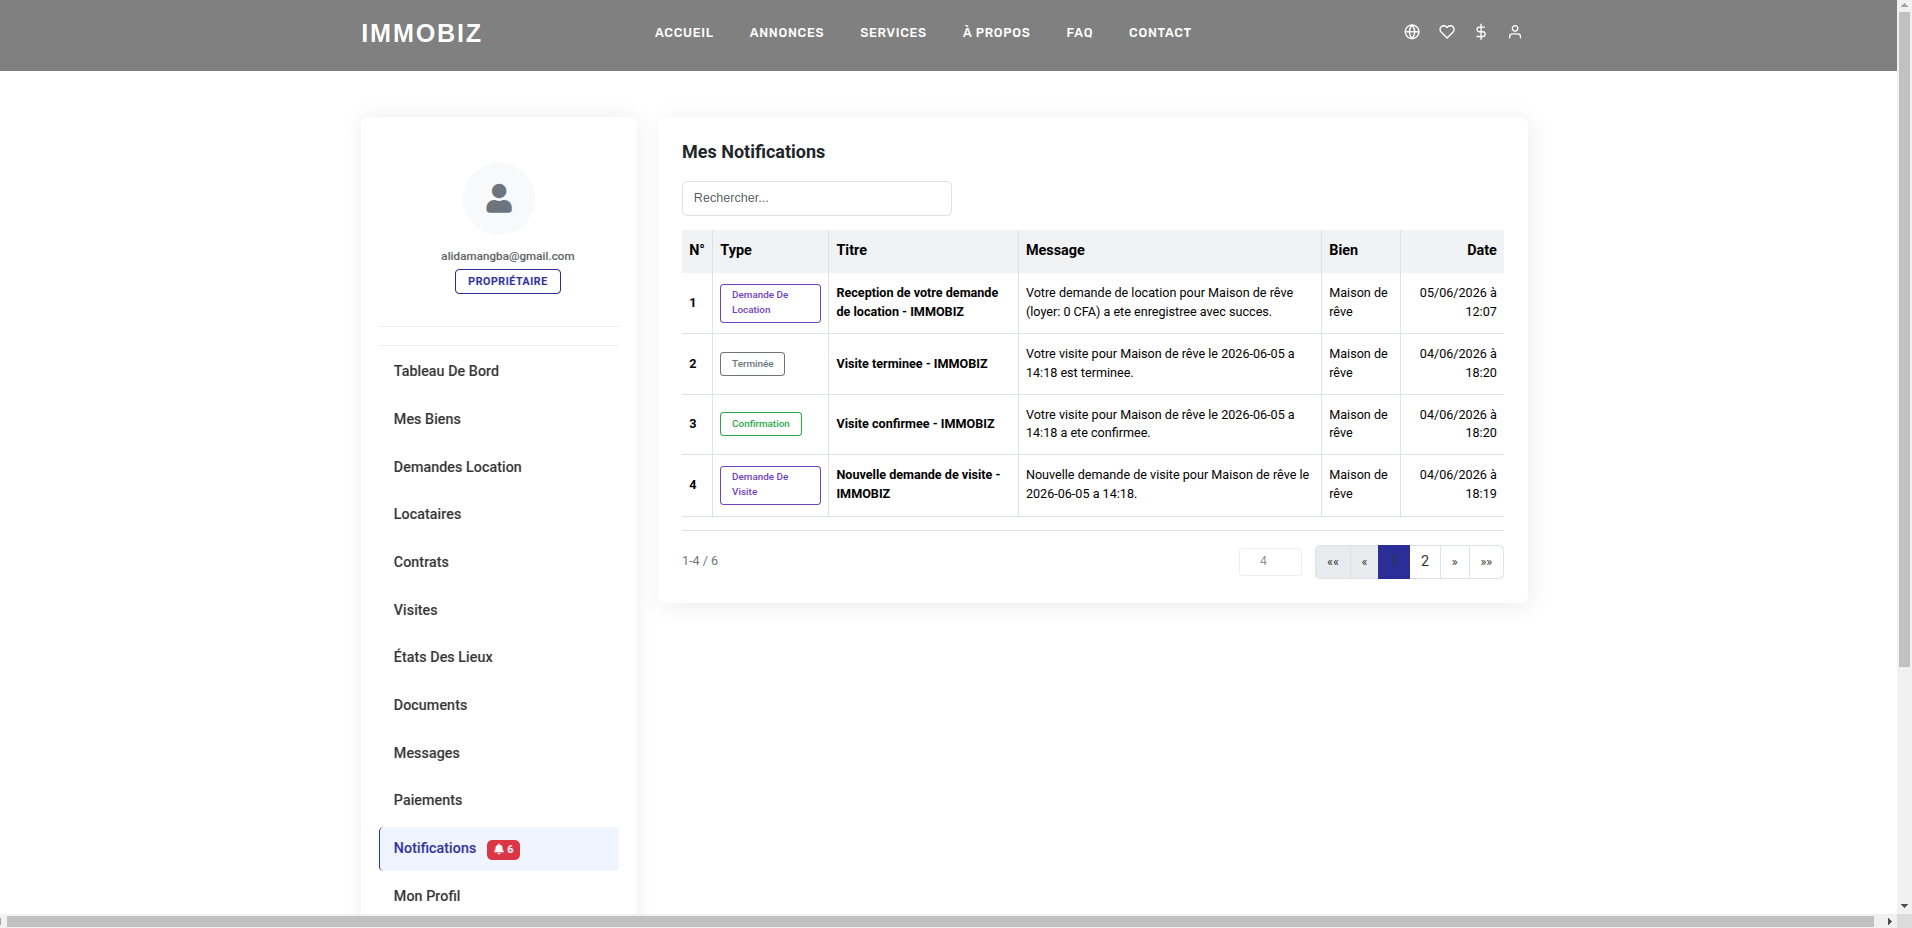
\includegraphics[width=\textwidth]{images/notification.png}
    \caption{Liste des notifications}
   
\end{figure}




\newpage

\subsection{Interface Locataire}

Après réception du courrier d'invitation reçu, le locataire crée son mot de passe afin d'accéder à son espace personnel, généré automatiquement par la plateforme.
\begin{figure}[H]
    \centering
        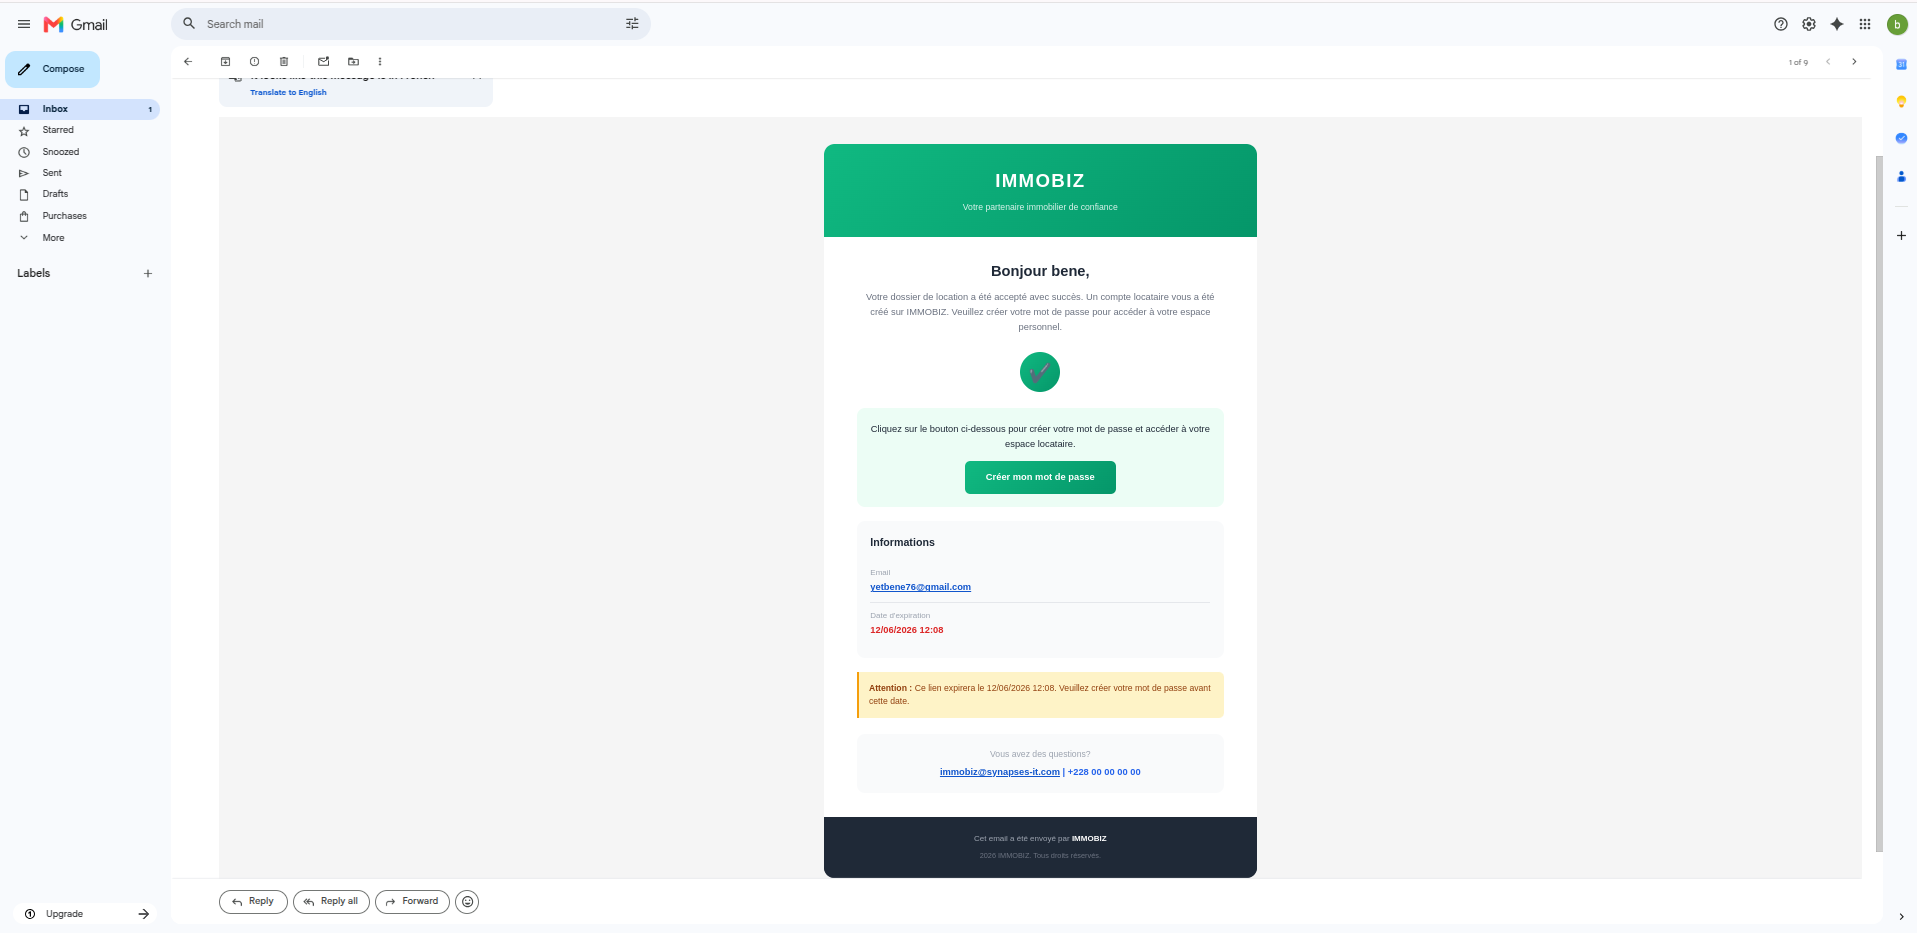
\includegraphics[width=\textwidth]{images/email-location2.png}
    \caption{L'email d'invitation pour la création du mot de passe}
    \label{fig:prospect-fiche-bien}
\end{figure}
\begin{figure}[H]
    \centering
        
\includegraphics[width=\textwidth]{images/email-location1.png}
    \caption{La création du mot de passe }
    \label{fig:prospect-fiche-bien}
\end{figure}

Une fois le mot de passe créé, le locataire accède à son espace personnel où le contrat de location est déjà disponible. Il n'a plus qu'à le signer et à procéder au paiement.

\newpage



Après cela, Voici quelques fonctionnalités accès auxquels il accès: 
\begin{figure}[H]
    \centering
        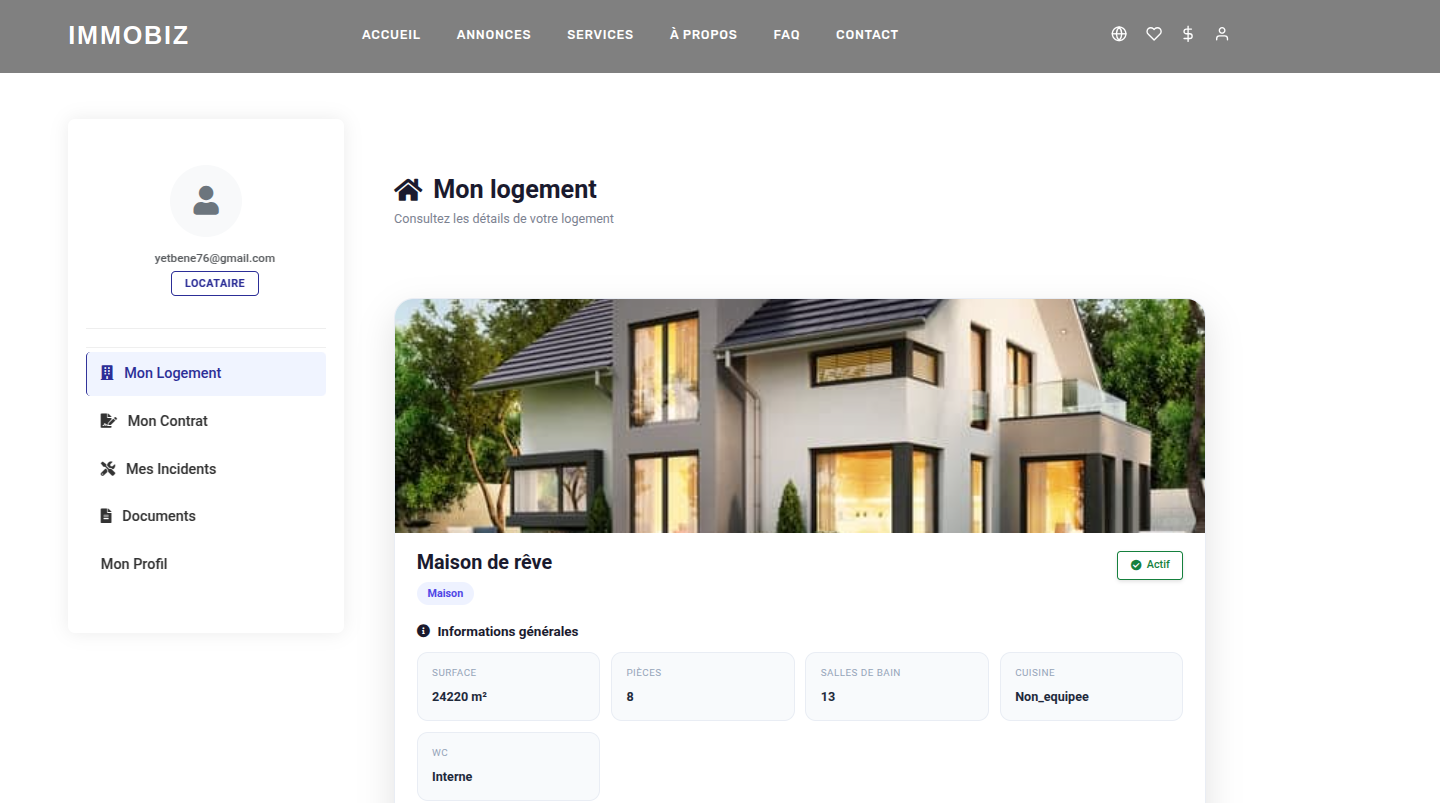
\includegraphics[width=\textwidth]{images/logement.png}
    \caption{Logement du locataire}
    \label{fig:prospect-fiche-bien}
\end{figure}


\begin{figure}[H]
    \centering
        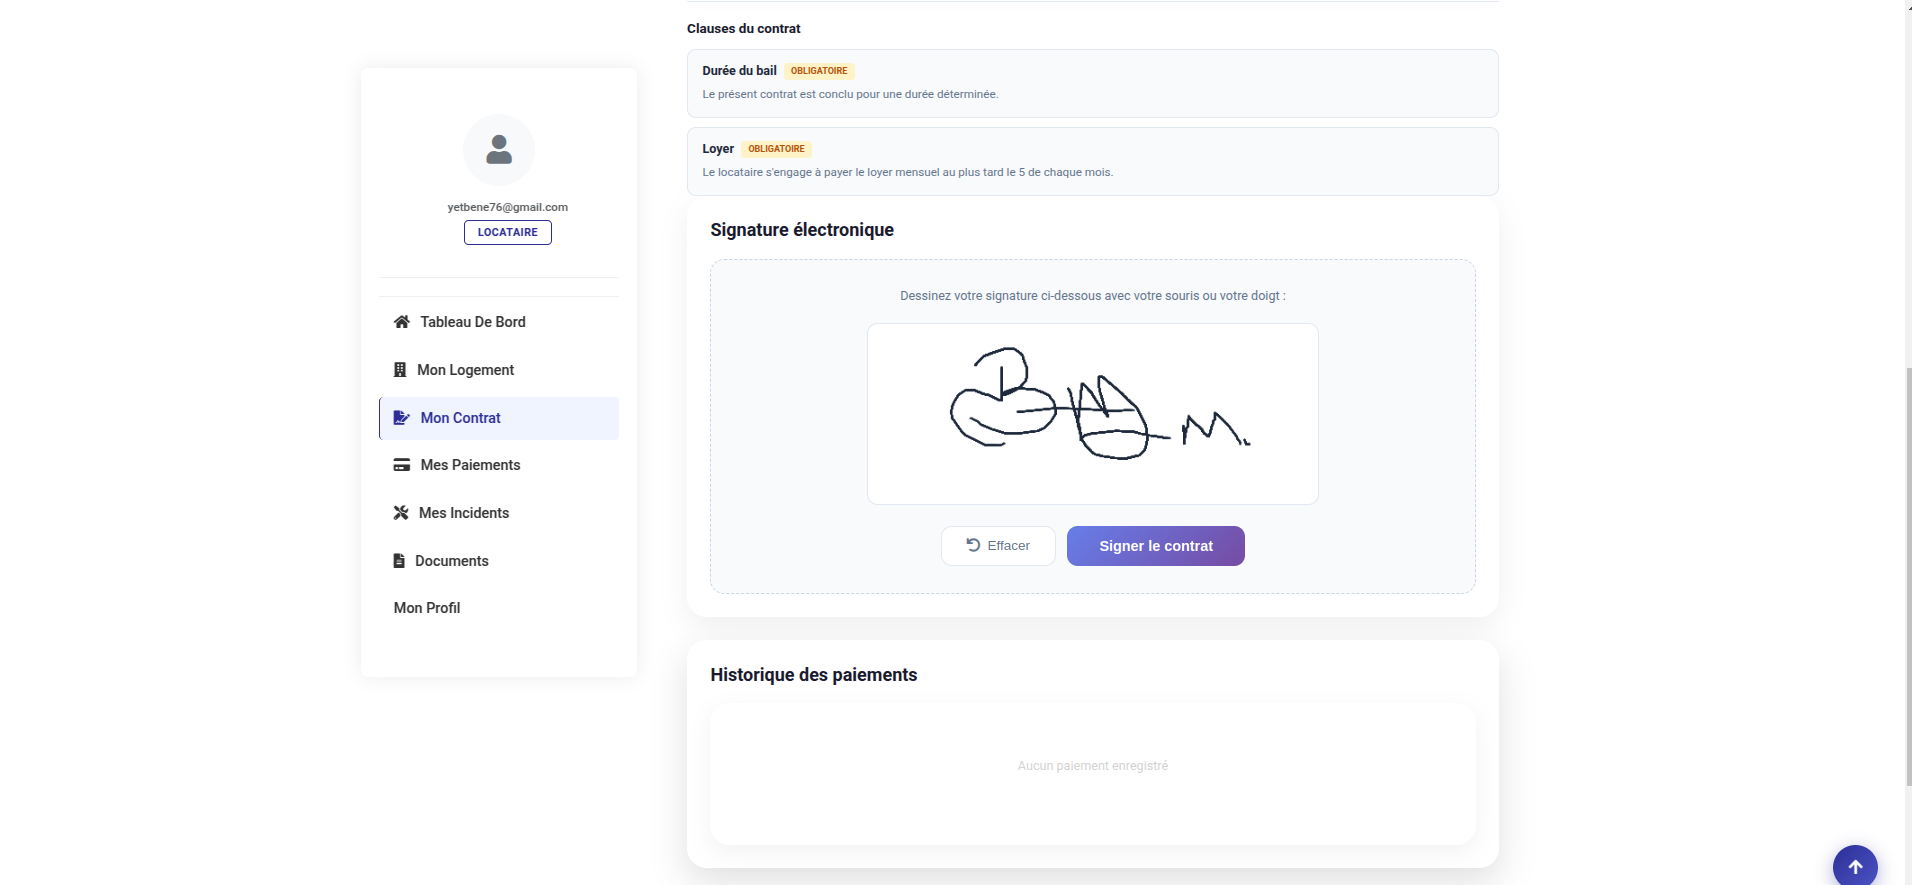
\includegraphics[width=\textwidth]{images/signer2.png}
    \caption{Signature du bail par le locataire}
    \label{fig:prospect-fiche-bien}
\end{figure}

Le contrat est signé par les deux parties : le locataire et le propriétaire s'engagent tous deux électroniquement depuis leurs espaces respectifs sur la plateforme.

\begin{figure}[H]
    \centering
        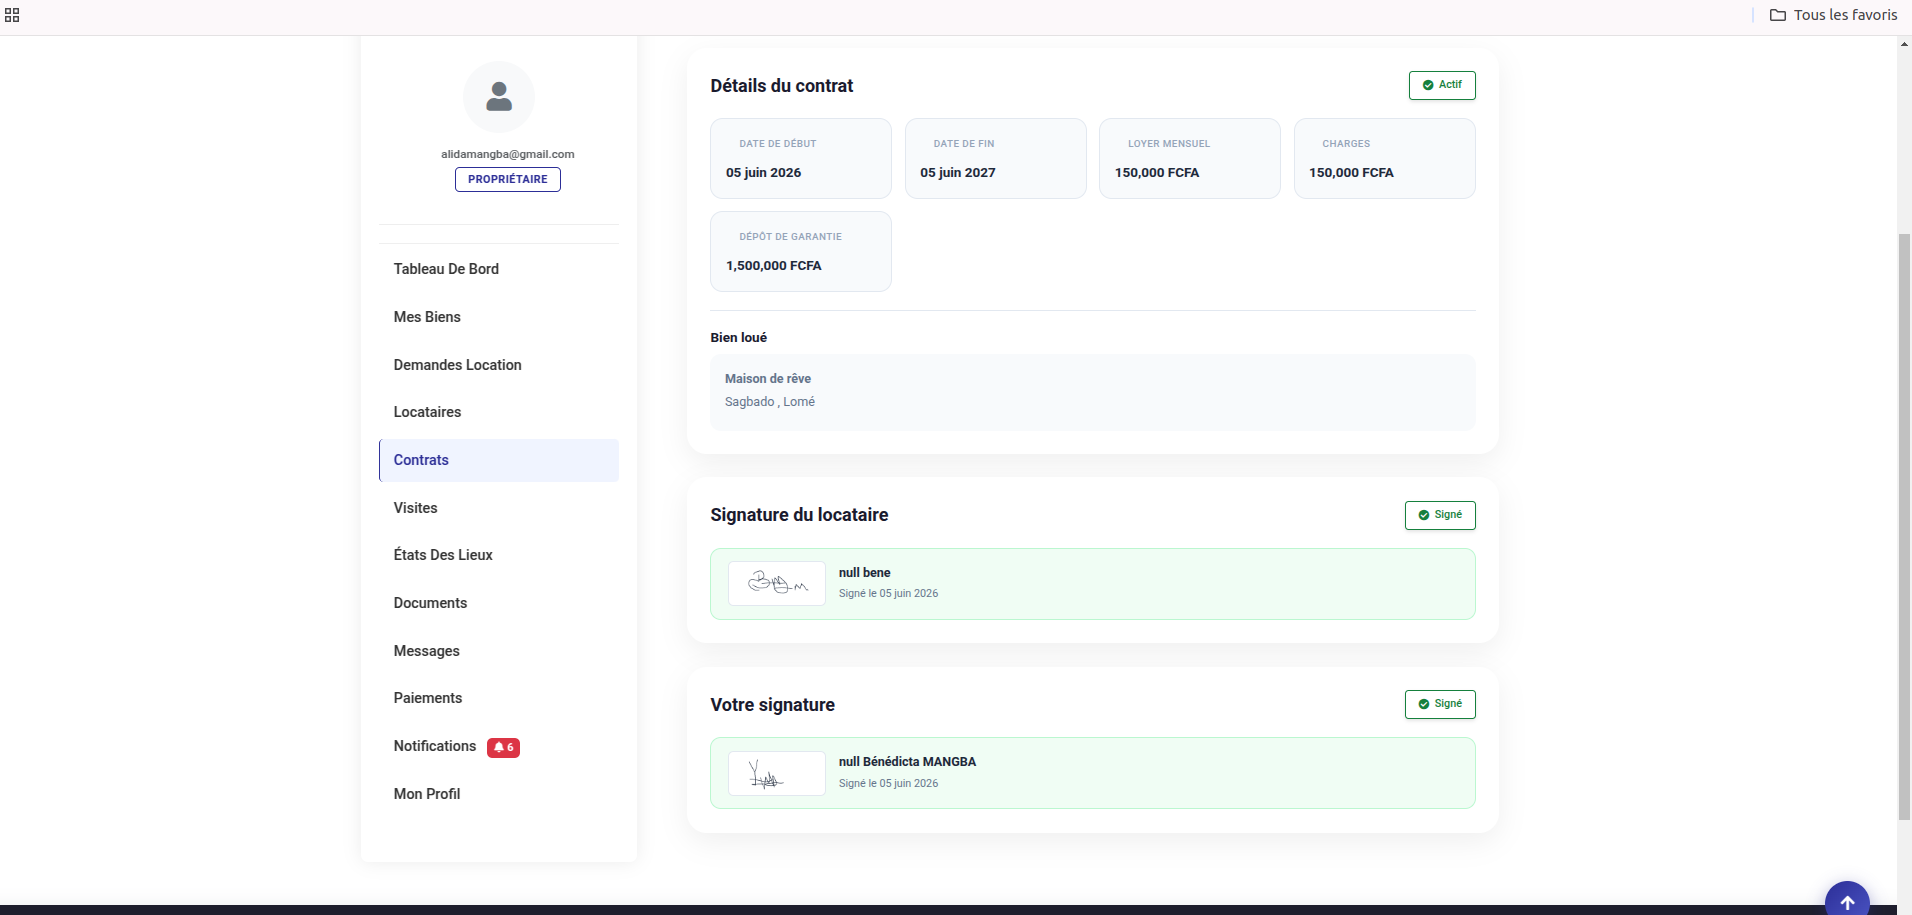
\includegraphics[width=\textwidth]{images/deuxpartit-contrat.png}
    \caption{Signature du bail par le locataire}
    \label{fig:prospect-fiche-bien}
\end{figure}



\begin{figure}[H]
    \centering
        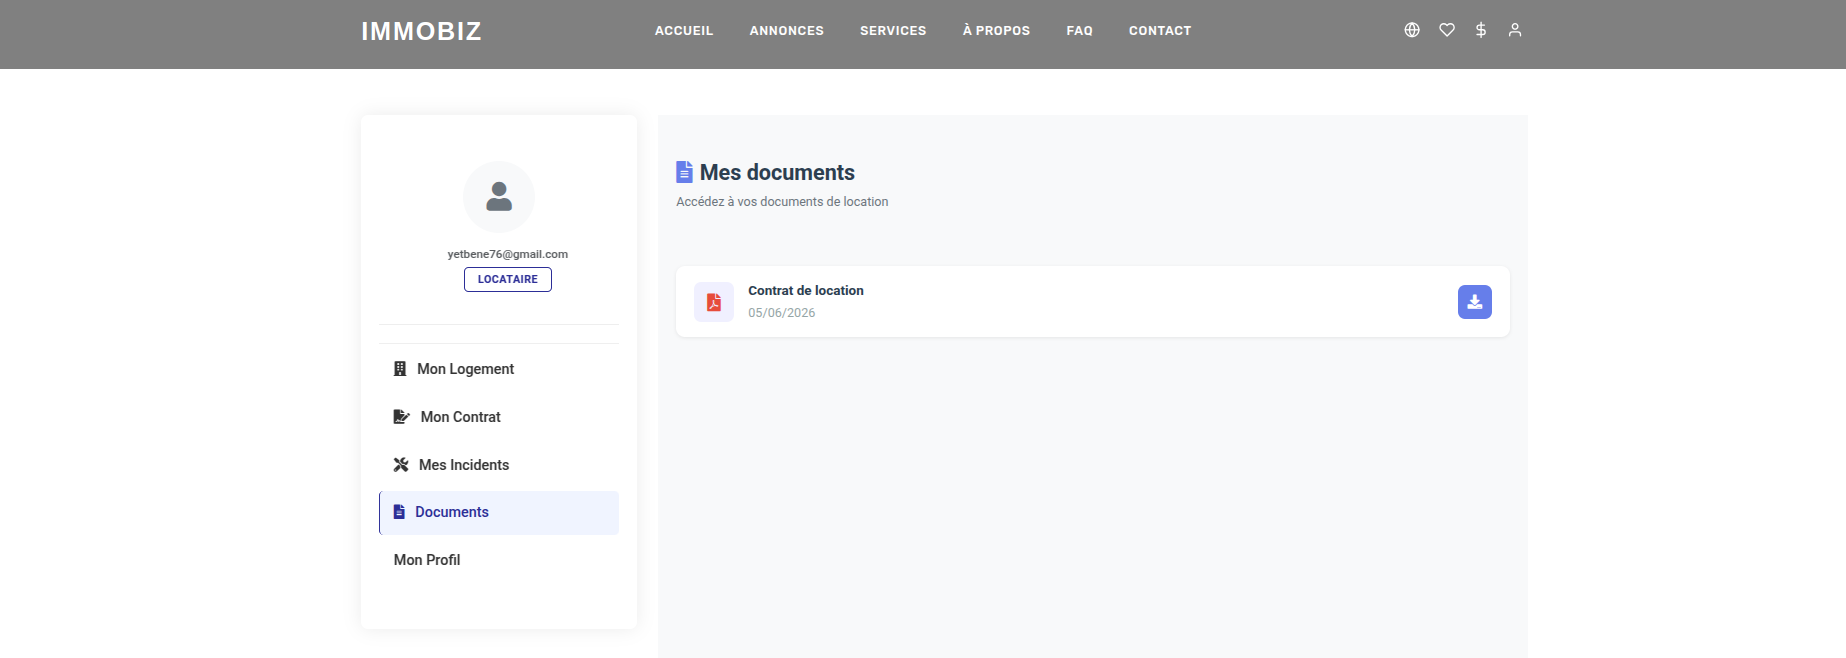
\includegraphics[width=\textwidth]{images/docu-locataire.png}
    \caption{liste de tous ses documents}
    \label{fig:prospect-fiche-bien}
\end{figure}

\begin{figure}[H]
    \centering
        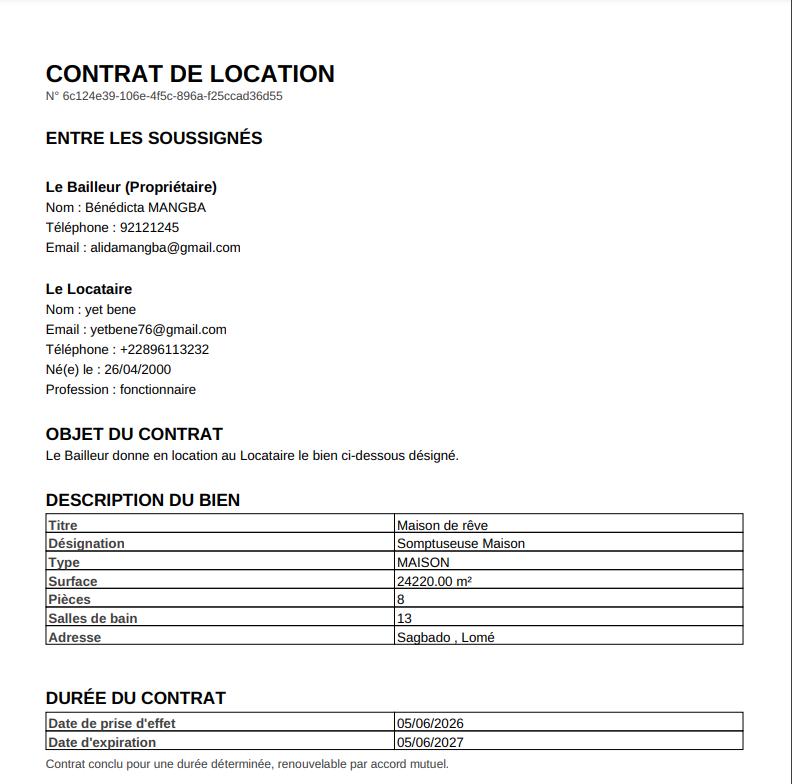
\includegraphics[width=\textwidth]{images/contrat-locataire-telecharger1.png}
    \label{fig:prospect-fiche-bien}
\end{figure}

\begin{figure}[H]
    \centering
        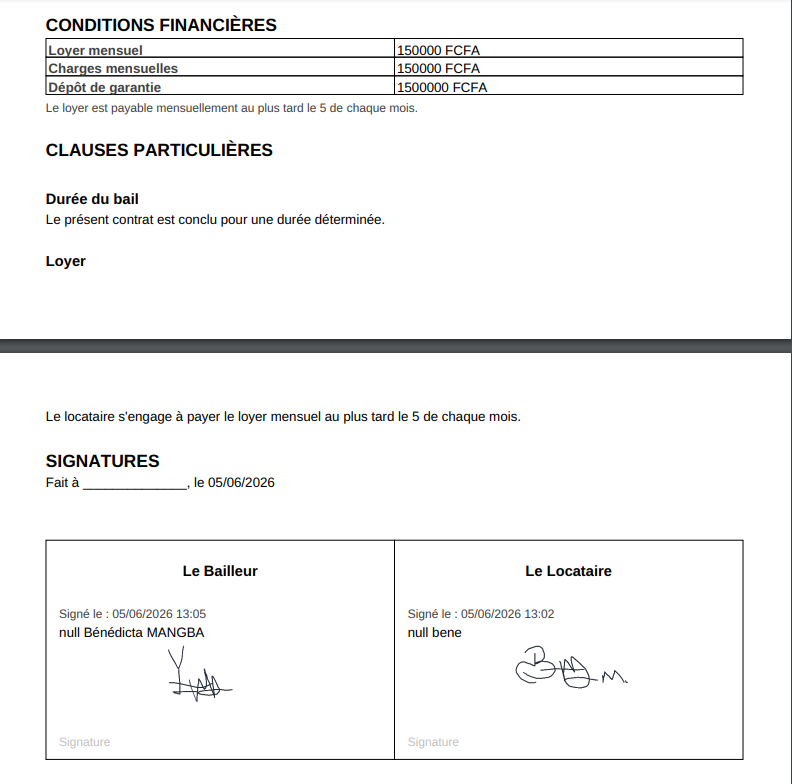
\includegraphics[width=\textwidth]{images/contrat-locataire-telecharger2.png}

    \caption{Document téléchargé par le locataire}
    \label{fig:prospect-fiche-bien}
\end{figure}


\begin{figure}[H]
    \centering
        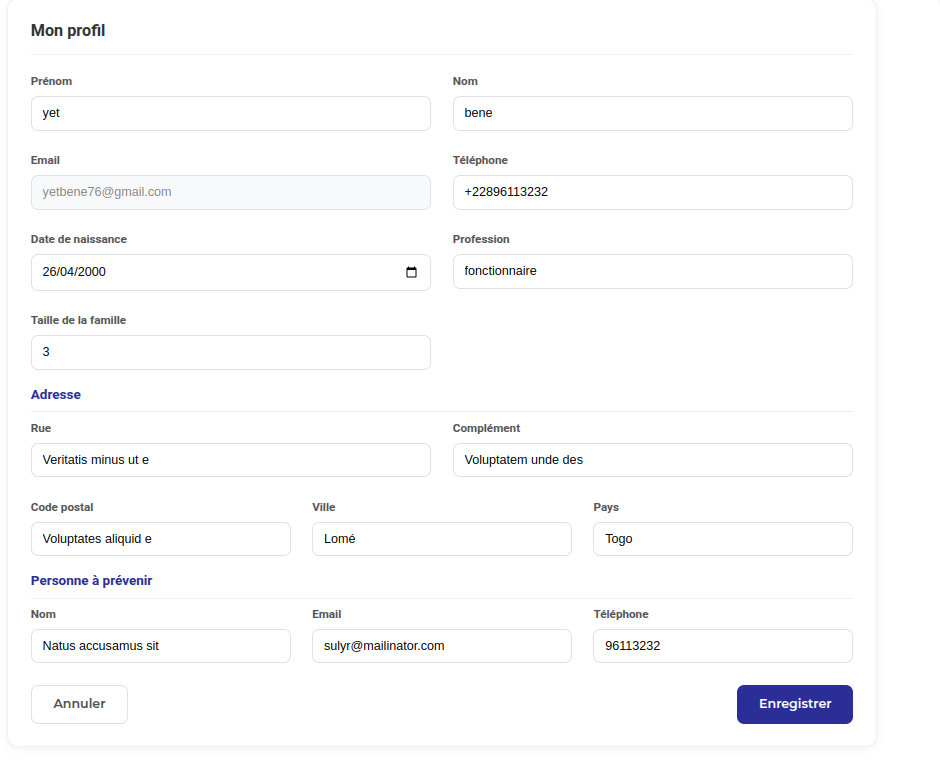
\includegraphics[width=\textwidth]{images/profile-locataire.png}
    \caption{Profil du locataire}
    \label{fig:prospect-fiche-bien}
\end{figure}

\begin{figure}[H]
    \centering
       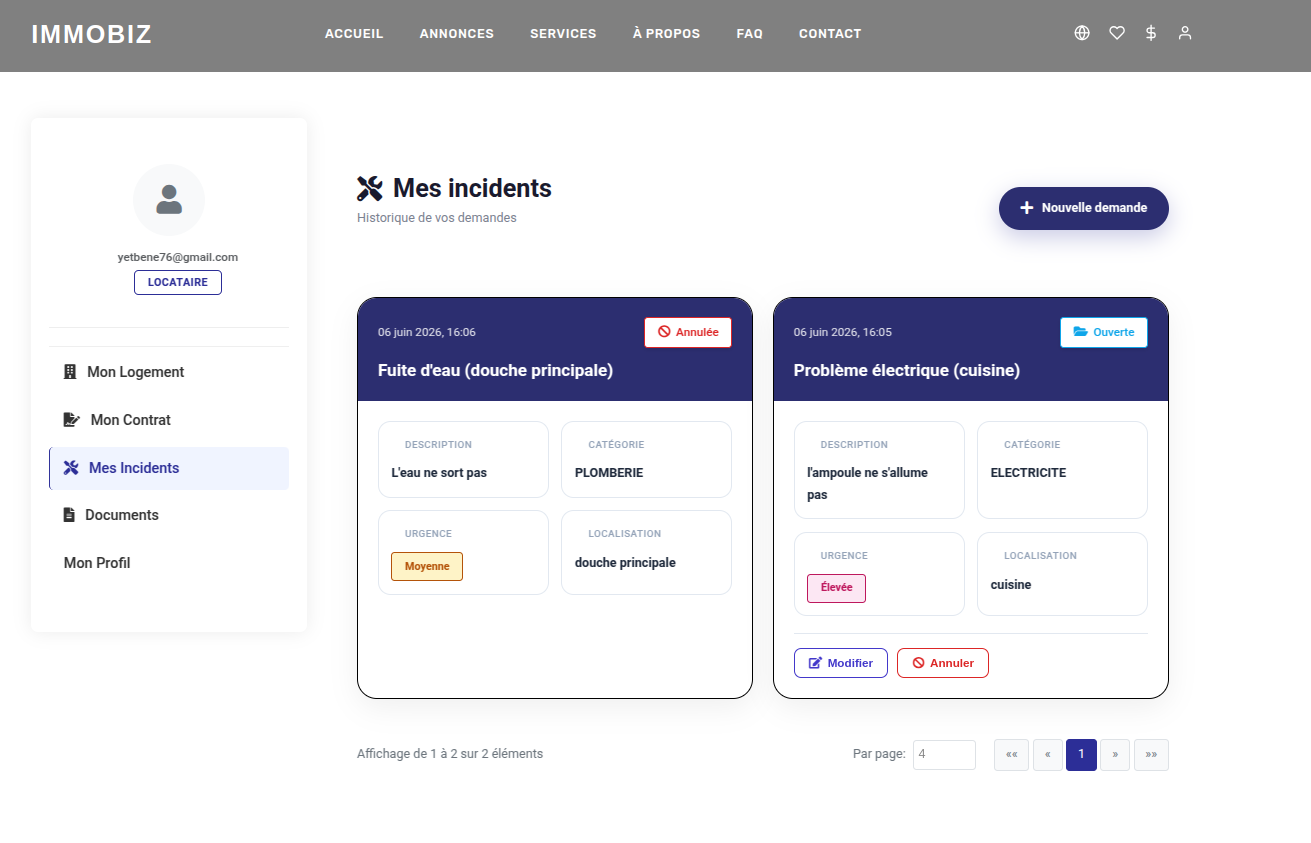
\includegraphics[width=\textwidth]{images/incident-locataire.png}
    \caption{Liste des incidents }
    \label{fig:prospect-fiche-bien}
\end{figure}



\newpage


\subsection{Interface du Gérant de la Plateforme}

La plateforme dispose également d'une interface dédiée au gérant à qui nous avons attribué le rôle \textbf{ADMINISTRATEUR}. 
Contrairement aux autres acteurs du système, l'administrateur bénéficie 
d'une vision globale sur l'ensemble des données de la plateforme : 
utilisateurs, biens, demandes, contrats, et transactions. Cependant, 
son rôle se limite à la supervision et à la consultation ; il n'a pas 
la possibilité de modifier ou de supprimer des éléments qui ne relèvent 
pas directement de sa responsabilité. Il intervient uniquement sur ce 
qui le concerne, garantissant ainsi l'intégrité des données de chaque 
acteur tout en maintenant une vue d'ensemble sur le bon fonctionnement 
de la plateforme.\\
\\

Lors de la connexion de l'administrateur, le tableau de bord présenté est illustré ci-dessous:




\begin{figure}[H]
    \centering
       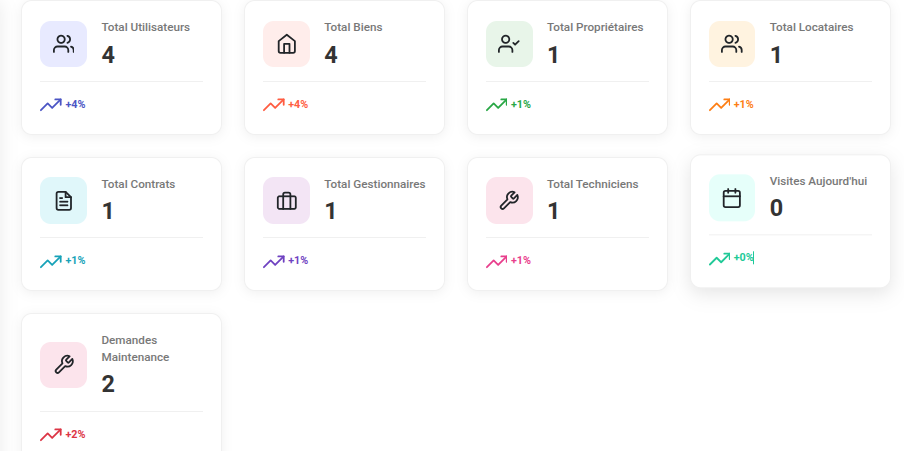
\includegraphics[width=\textwidth]{images/bor1.png}
        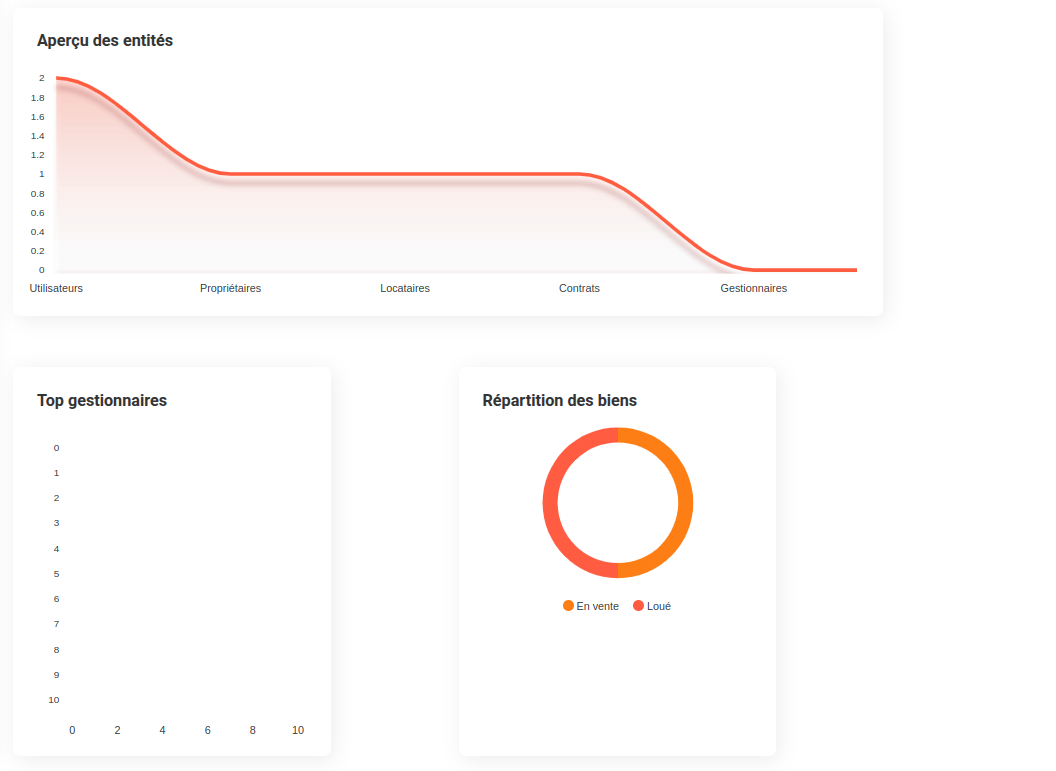
\includegraphics[width=\textwidth]{images/sahboard-admin1.png}
	  \caption{Le tableau de bord de l'administrateur}
    \label{fig:prospect-fiche-bien}
\end{figure}
\newpage


\begin{figure}[H]
    \centering
       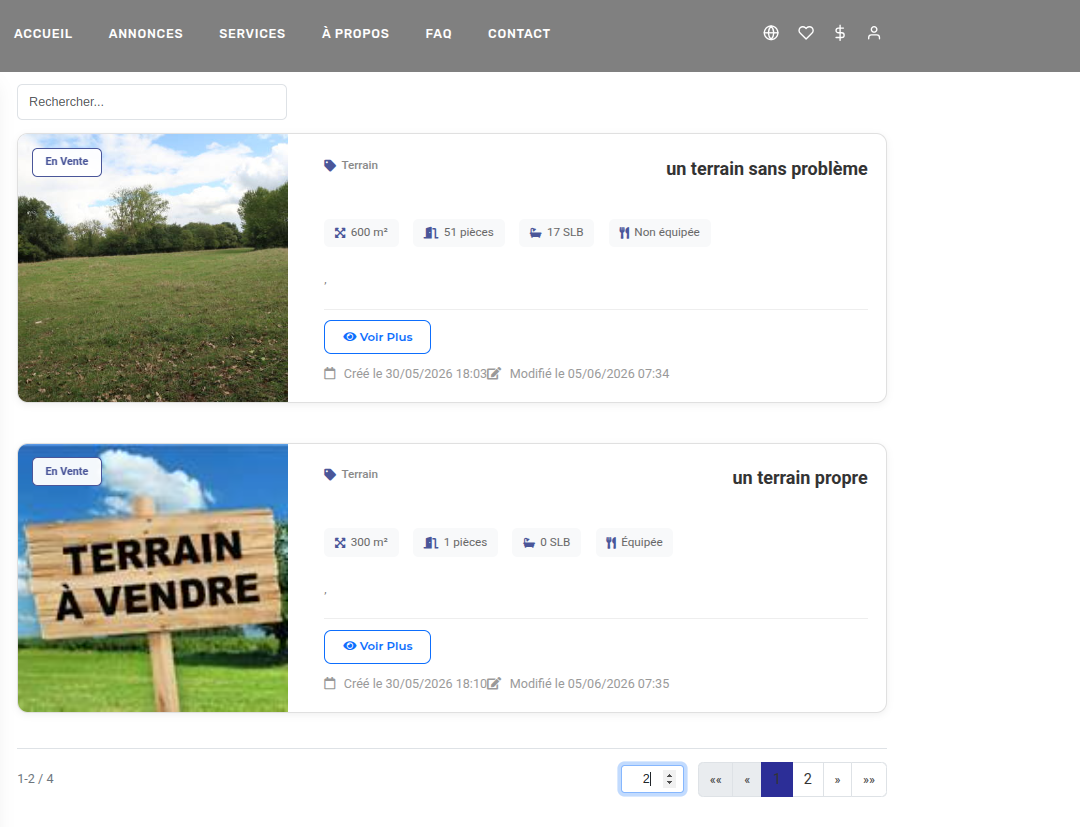
\includegraphics[width=\textwidth]{images/bien-admin.png}
    \caption{Liste des Biens immobiliers consultables par le gérant de la plateforme}
    \label{fig:prospect-fiche-bien}
\end{figure}




\begin{figure}[H]
    \centering
       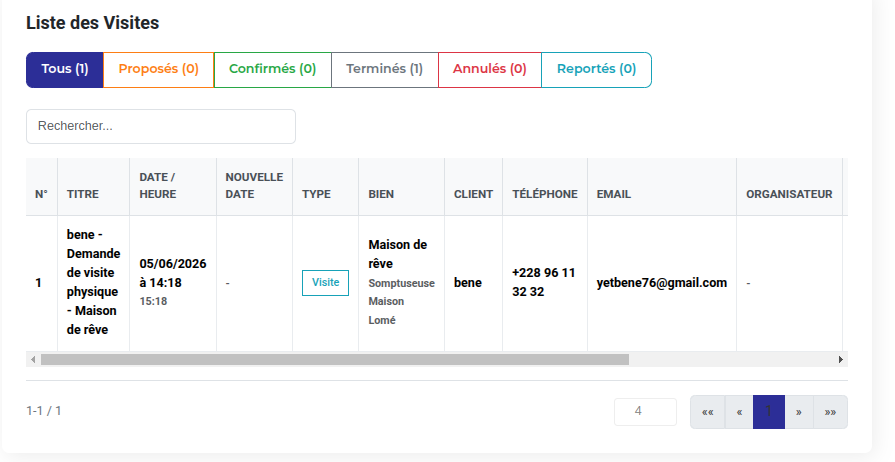
\includegraphics[width=\textwidth]{images/admin-visite.png}
    \caption{La liste des visites}
    \label{fig:prospect-fiche-bien}
\end{figure}

\newpage

\begin{figure}[H]
    \centering
       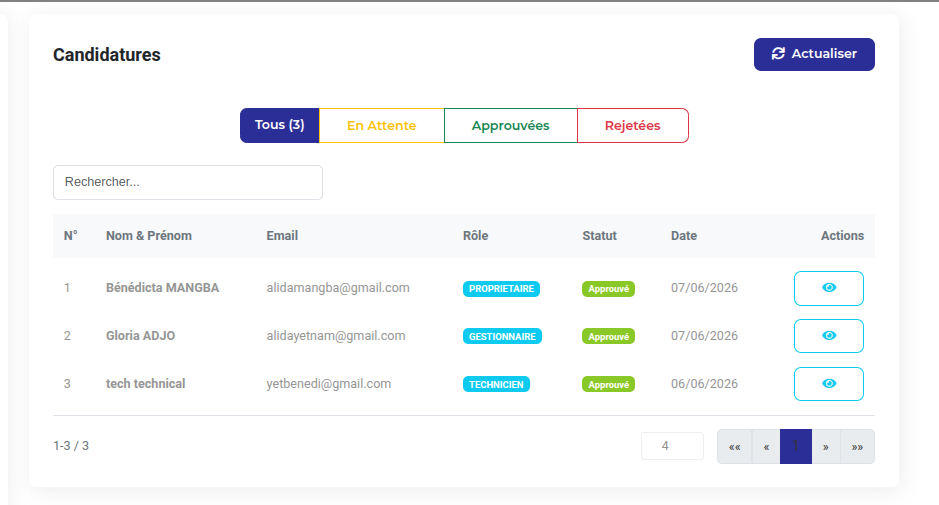
\includegraphics[width=\textwidth]{images/candidature.png}
    \caption{La liste des candidatures}
    \label{fig:prospect-fiche-bien}
\end{figure}


\begin{figure}[H]
    \centering
       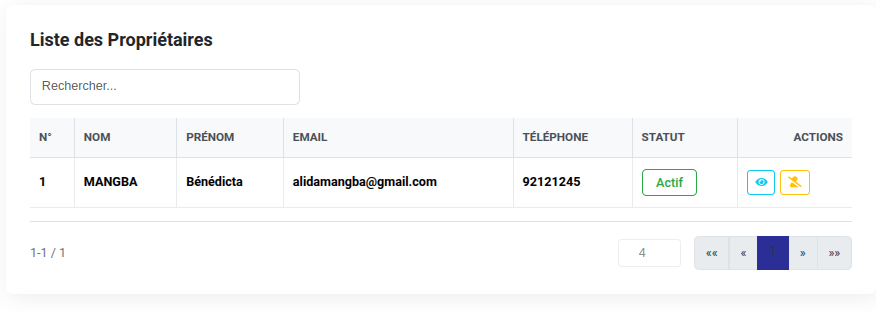
\includegraphics[width=\textwidth]{images/propretaire.png}
    \caption{Liste des propriétaires}
    \label{fig:prospect-fiche-bien}
\end{figure}

\begin{figure}[H]
    \centering
       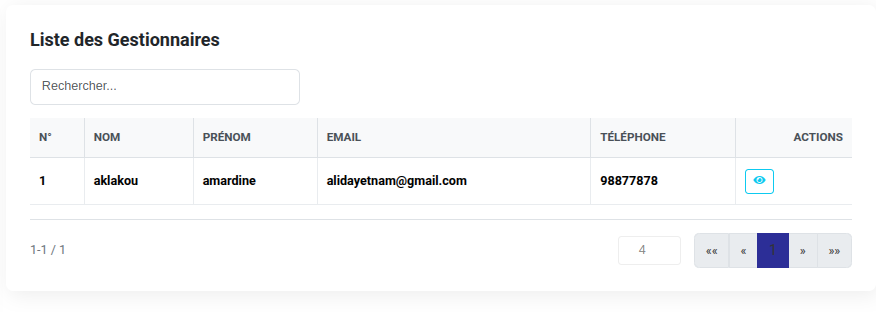
\includegraphics[width=\textwidth]{images/ges.png}
    \caption{Liste des gestionnaires}
    \label{fig:prospect-fiche-bien}
\end{figure}

\begin{figure}[H]
    \centering
       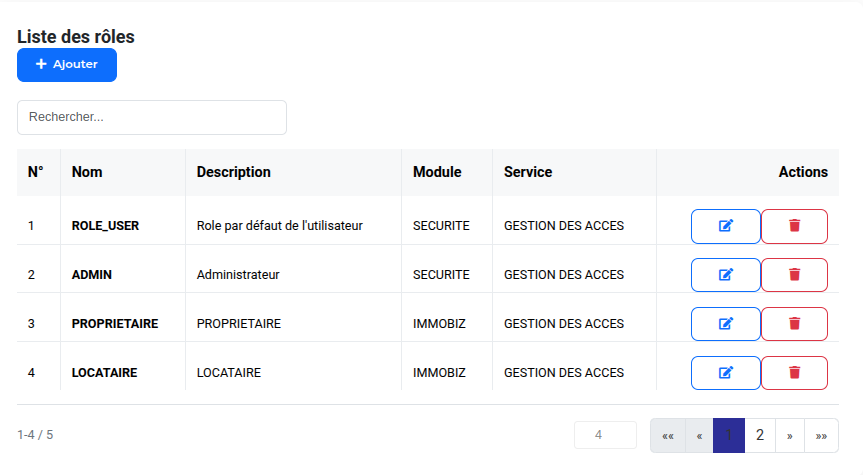
\includegraphics[width=\textwidth]{images/role.png}
    \caption{Liste des rôles}
    \label{fig:prospect-fiche-bien}
\end{figure}

\begin{figure}[H]
    \centering
       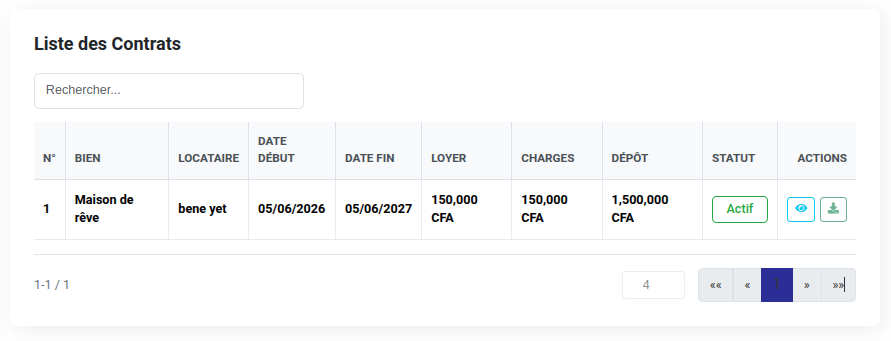
\includegraphics[width=\textwidth]{images/contrat-admin.png}
    \caption{Liste des contrats}
    \label{fig:prospect-fiche-bien}
\end{figure}


\begin{figure}[H]
    \centering
       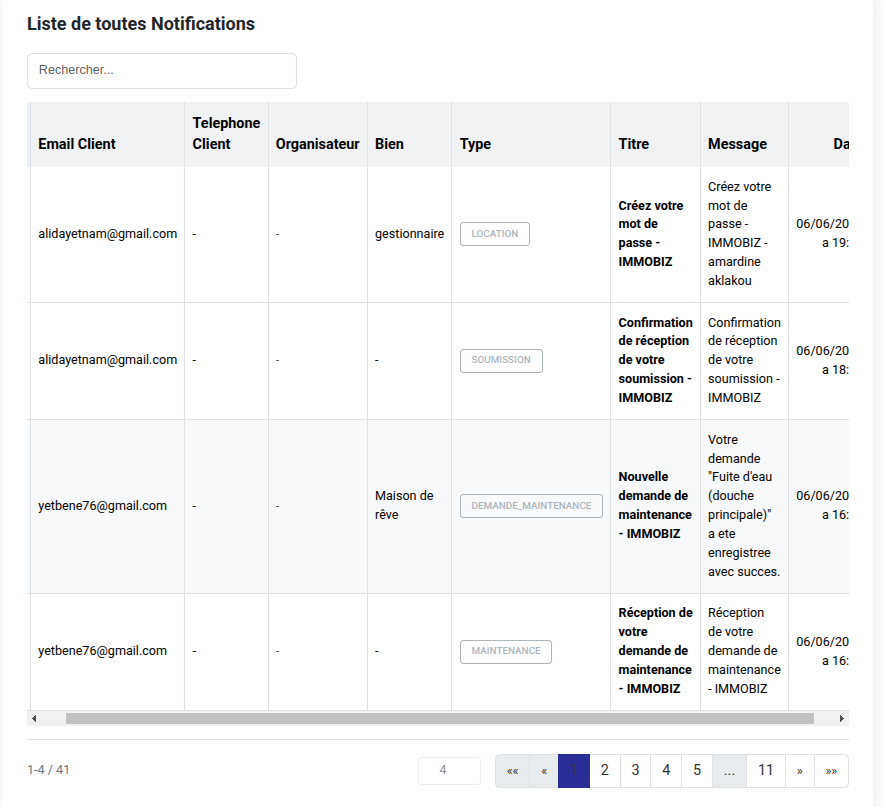
\includegraphics[width=\textwidth]{images/notifi.png}
    \caption{Liste des notifications}
    \label{fig:prospect-fiche-bien}
\end{figure}

\begin{figure}[H]
    \centering
       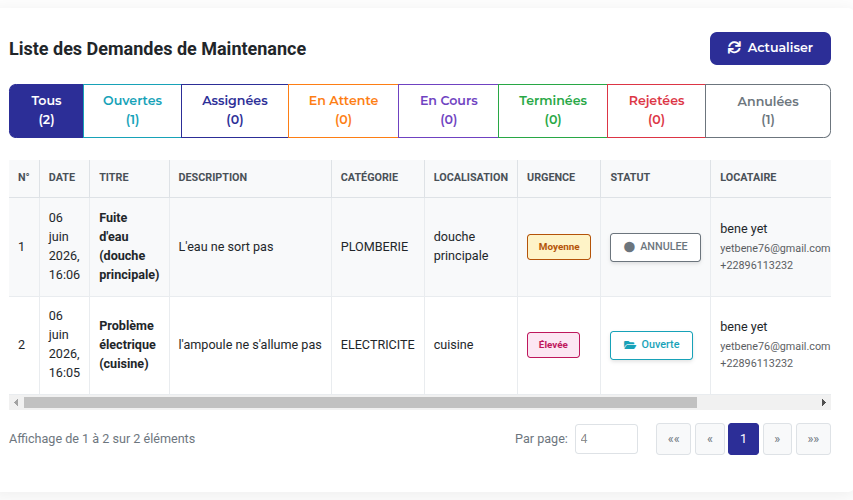
\includegraphics[width=\textwidth]{images/demande-ad.png}
    \caption{Liste des demandes de maintenance}
    \label{fig:prospect-fiche-bien}
\end{figure}



\begin{figure}[H]
    \centering
       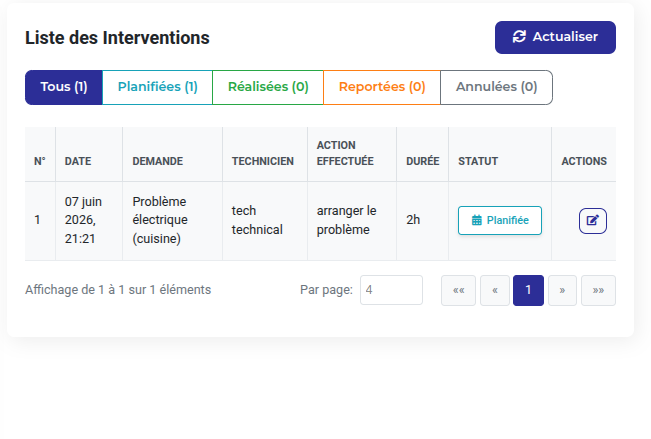
\includegraphics[width=\textwidth]{images/intervention-ad.png}
	  \caption{La liste des interventions}
    \label{fig:prospect-fiche-bien}
\end{figure}


\begin{figure}[H]
    \centering
       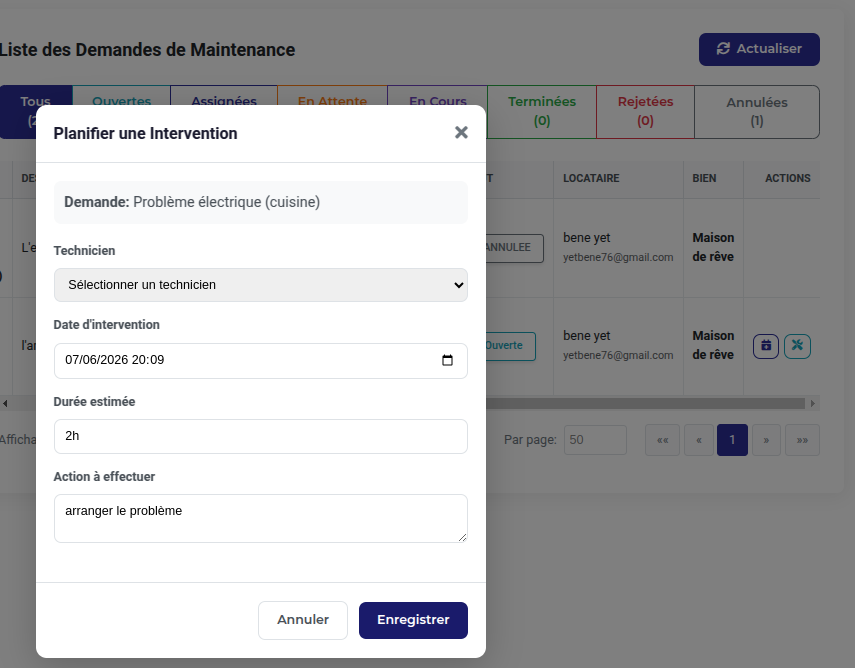
\includegraphics[width=\textwidth]{images/plani-intervention}
    \caption{Planification de l'intervention}
    \label{fig:prospect-fiche-bien}
\end{figure}

\begin{figure}[H]
    \centering
       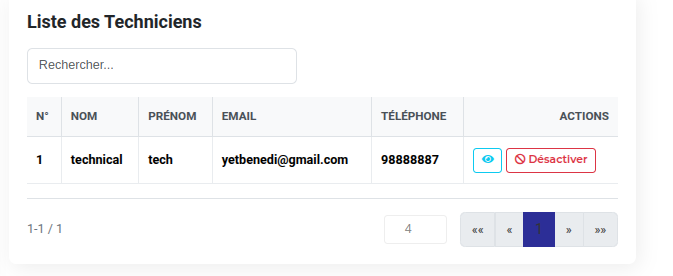
\includegraphics[width=\textwidth]{images/technicien.png}
	  \caption{La liste des techniciens}
    \label{fig:prospect-fiche-bien}
\end{figure}

\newpage

\subsection{Interface Technicien}

\begin{figure}[H]
    \centering
       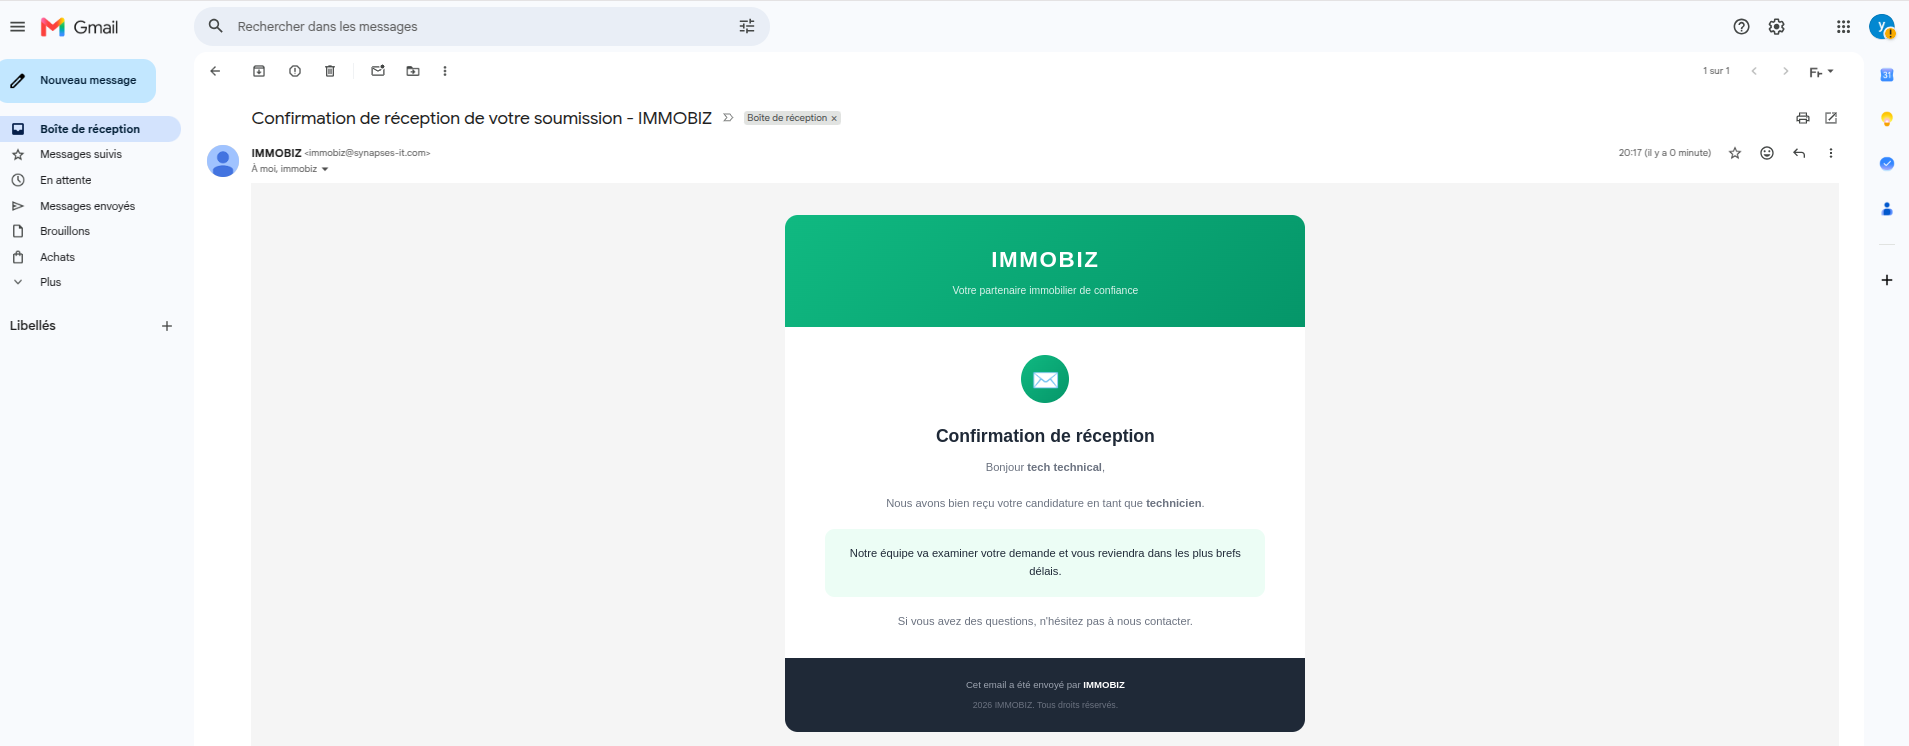
\includegraphics[width=\textwidth]{images/reception-tech.png}
	  \caption{Émail de réception de la candidature du technicien}
    \label{fig:prospect-fiche-bien}
\end{figure}


\begin{figure}[H]
    \centering
       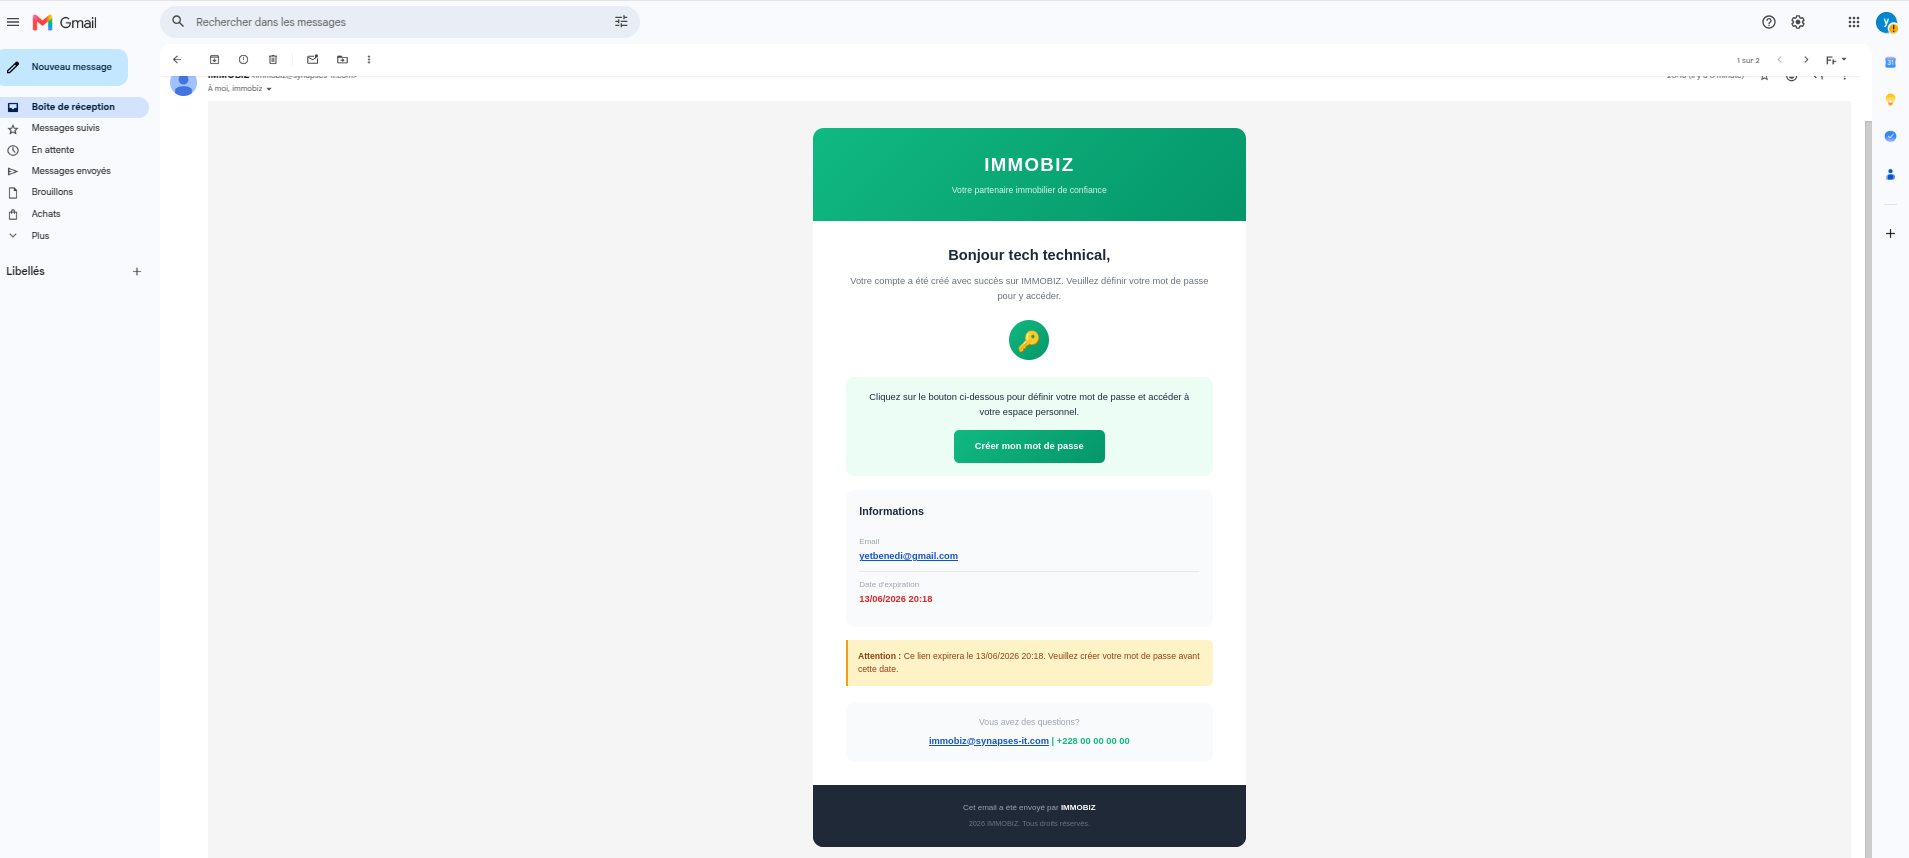
\includegraphics[width=\textwidth]{images/email-validation-teh.png}
	  \caption{Émail de validation du compte et d'invitation à la création du mot de passe }
    \label{fig:prospect-fiche-bien}
\end{figure}

\begin{figure}[H]
    \centering
       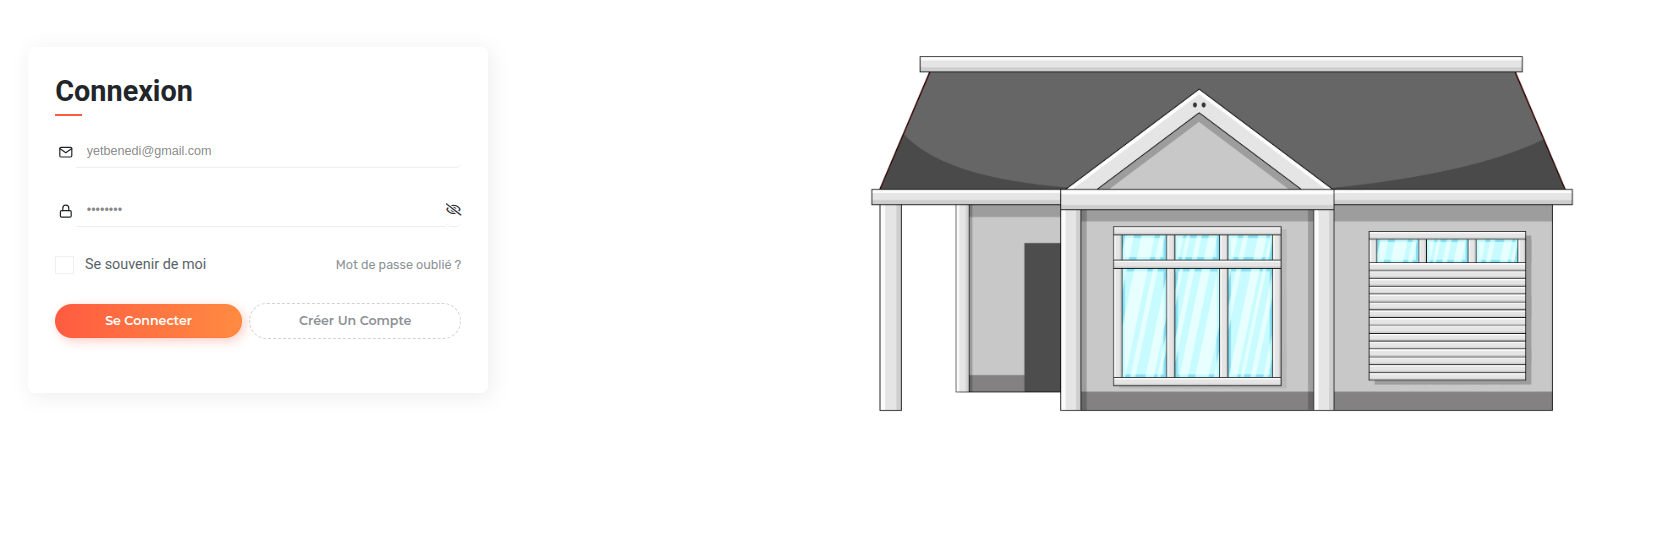
\includegraphics[width=\textwidth]{images/creationpasse-technicien.png}
	  \caption{Émail de validation du compte et d'invitation à la création du mot de passe }
    \label{fig:prospect-fiche-bien}
\end{figure}

\begin{figure}[H]
    \centering
       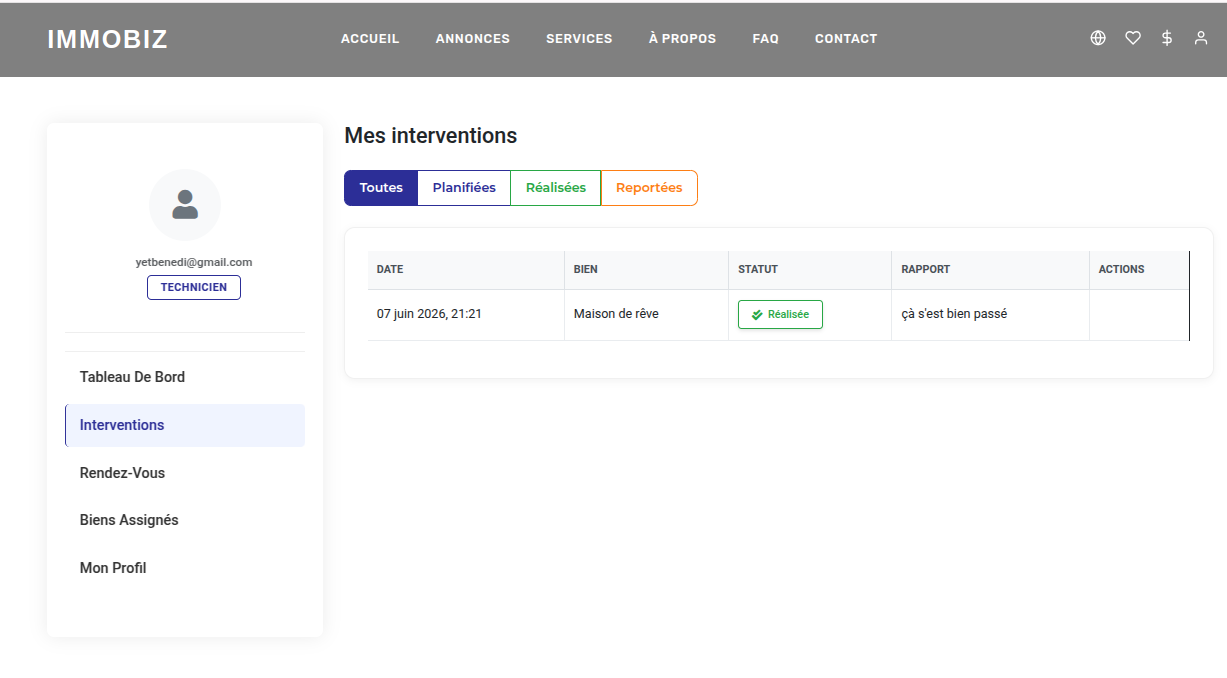
\includegraphics[width=\textwidth]{images/intervention-tech.png}
	  \caption{Liste des interventions liées au technicien}
    \label{fig:prospect-fiche-bien}
\end{figure}


\begin{figure}[H]
    \centering
       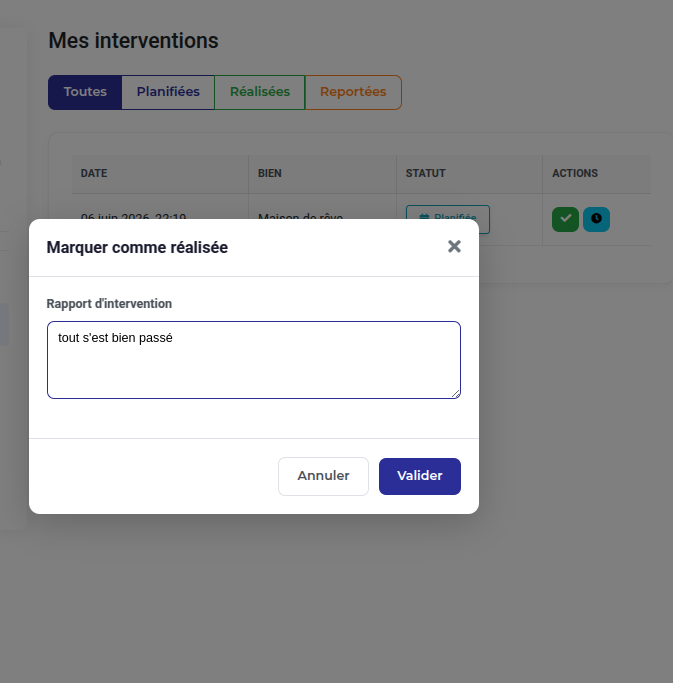
\includegraphics[width=\textwidth]{images/rapport-tech.png}
	  \caption{Rapport du technicien }
    \label{fig:prospect-fiche-bien}
\end{figure}


\begin{figure}[H]
    \centering
       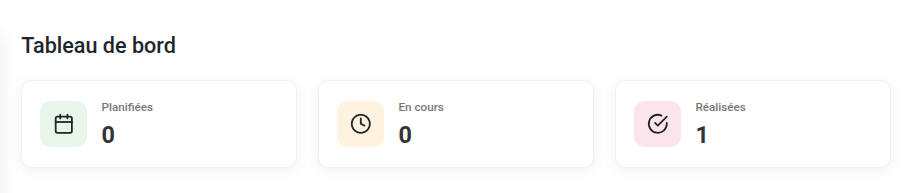
\includegraphics[width=\textwidth]{images/bord-tech.png}
	  \caption{Tableau de bord du technicien }
\end{figure}

\begin{figure}[H]
    \centering
       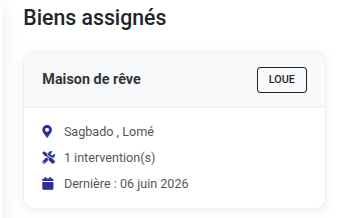
\includegraphics[width=0.50\textwidth]{images/bien-tech.png}
	  \caption{Biens assignés au technicien }
    \label{fig:prospect-fiche-bien}
\end{figure}

\begin{figure}[H]
    \centering
       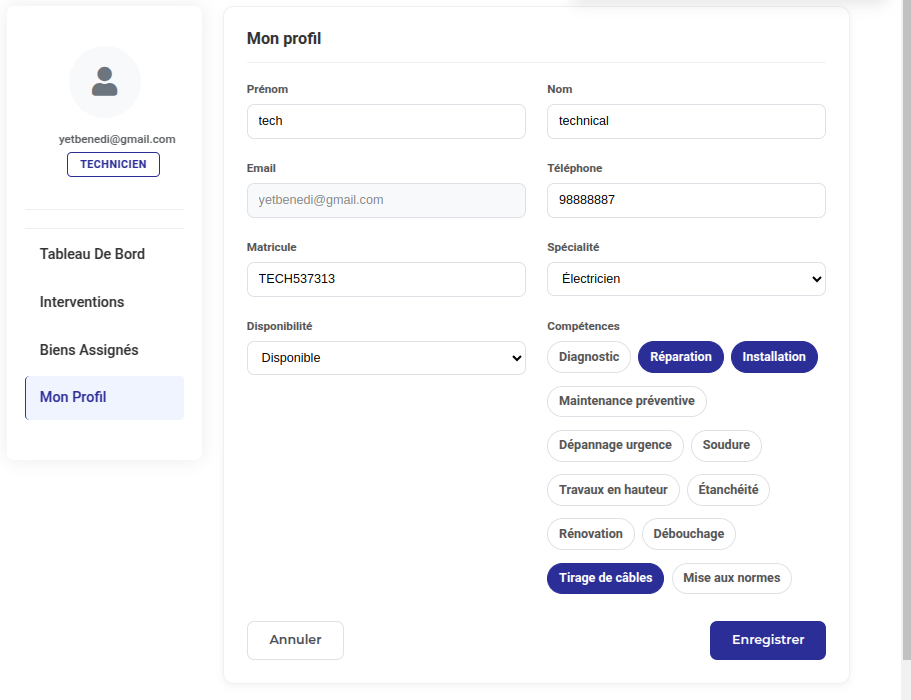
\includegraphics[width=\textwidth]{images/profil-tech.png}
	  \caption{ Profil technicien }
    \label{fig:prospect-fiche-bien}
\end{figure}

\newpage

\subsection{Interface Agence Immobilière}

Cette interface offre à l'agence un espace centralisé pour la gestion locative, de la création des comptes gestionnaires au suivi des biens, des visites et des opérations financières.
Dans cette section, nous commencerons par détailler le menu latéral (sidebar)


\begin{figure}[H]
    \centering
       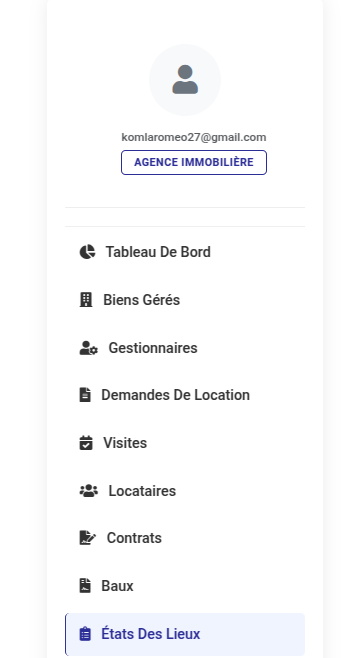
\includegraphics[width=0.60\textwidth]{images/sidebar-agence1.png} 
\end{figure}

\newpage
\begin{figure}[H]
    \centering
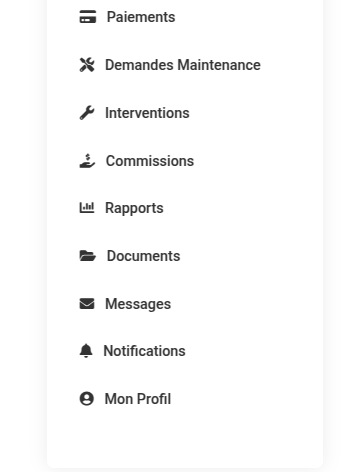
\includegraphics[width=0.60\textwidth]{images/sidebar-agence3.png}
	  \caption{ Menu latéral de l'agence Immobilière  }
    \label{fig:prospect-fiche-bien}
\end{figure}


Le menu latéral(sidebar) de l'interface agence se structure en sept catégories :

\vspace{0.3cm}

\begin{itemize}
    \item \motcle{Gestion des biens} : Biens gérés
    \item \motcle{Personnes} : Gestionnaires, Locataires
    \item \motcle{Opérations} : Demandes de location, Visites, Contrats, Baux, États des lieux
    \item \motcle{Finances} : Paiements, Commissions
    \item \motcle{Communication} : Messages, Notifications
    \item \motcle{Support} : Maintenance, Interventions
    \item \motcle{Gestion interne} : Documents, Rapports
\end{itemize}



\subsubsection{Gestion des gestionnaires}

L'agence immobilière peut créer et administrer ses gestionnaires directement depuis la plateforme \motcle{IMMOBIZ}.

\begin{infobox}
\textbf{Création d'un gestionnaire}

L'agence remplit un formulaire renseignant les informations du gestionnaire. Une fois le formulaire validé, le
système \textbf{crée automatiquement} le compte et envoie un courrier
électronique contenant un lien d'activation permettant au gestionnaire de
définir lui-même son mot de passe.
\end{infobox}

\begin{figure}[H]
    \centering
       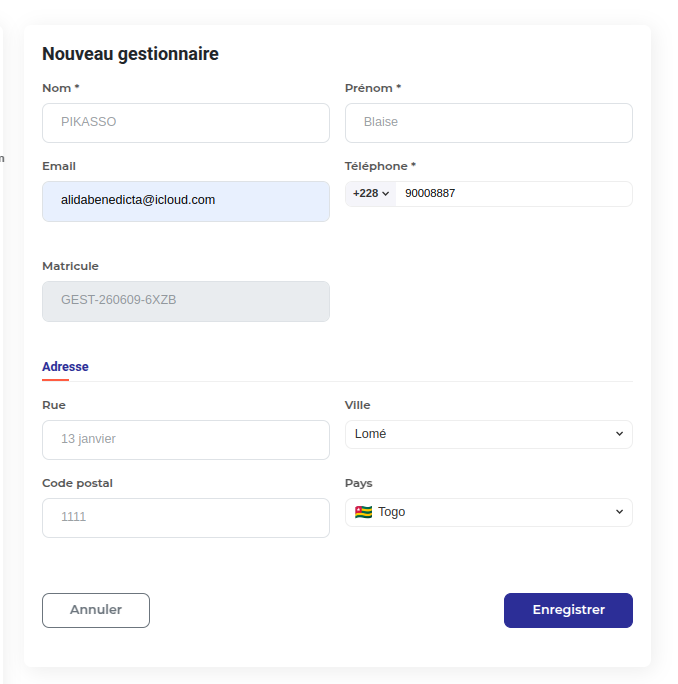
\includegraphics[width=\textwidth]{images/compte-ges.png}
	  \caption{ Création de compte du gestionnaire }
    \label{fig:prospect-fiche-bien}
\end{figure}

\begin{figure}[H]
    \centering
       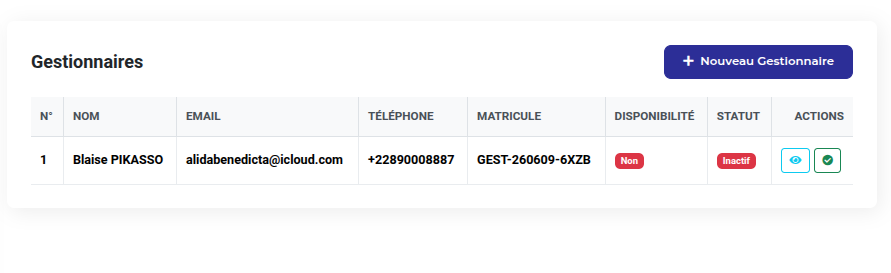
\includegraphics[width=\textwidth]{images/liste-ges.png}
	  \caption{ Liste des gestionnaires}
    \label{fig:prospect-fiche-bien}
\end{figure}


\vspace{0.3cm}

\begin{accentbox}
\textbf{Cycle d'activation du compte}

\vspace{0.2cm}

Tant que le gestionnaire n'a pas cliqué sur le lien et défini son mot de
passe, son compte demeure \important{inactif} et indisponible sur la
plateforme. Dès la confirmation du mot de passe, le compte bascule
automatiquement à l'état \textcolor{vertvalid}{\textbf{actif}}, rendant
le gestionnaire immédiatement opérationnel.
\end{accentbox}

\begin{figure}[H]
    \centering
       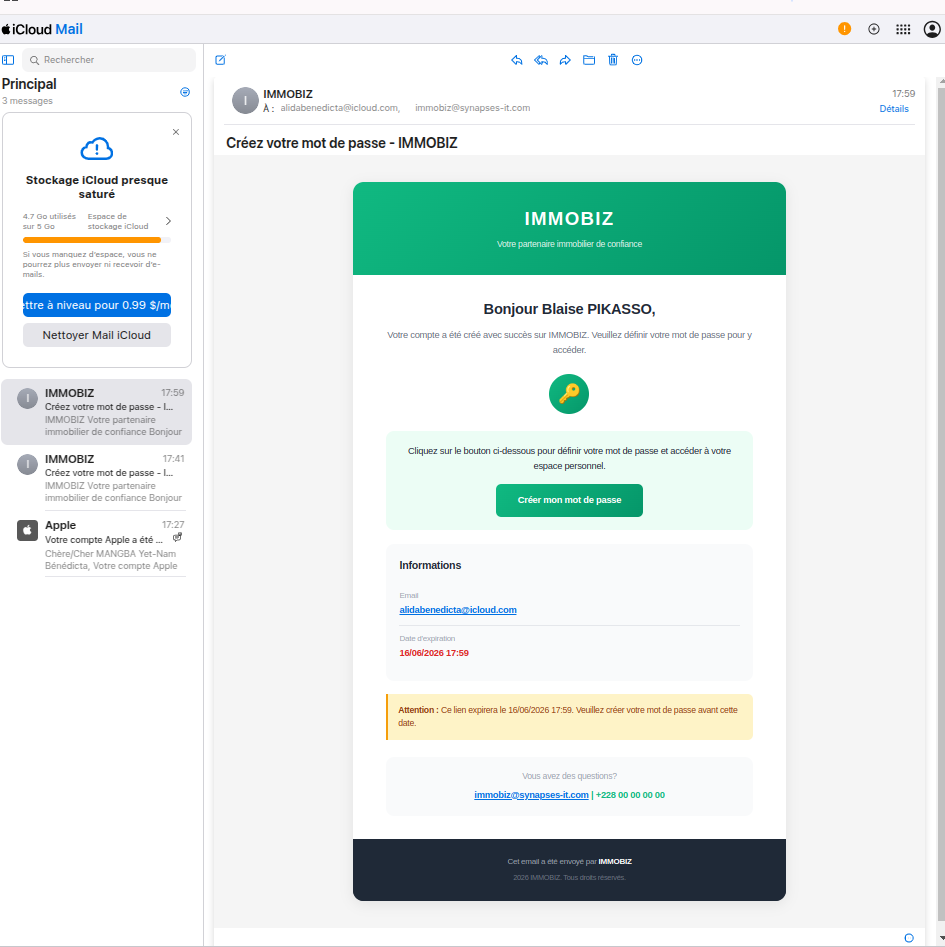
\includegraphics[width=0.60\textwidth]{images/message-ges.png}
	  \caption{ Email d'activation du compte du gestionnaire }
    \label{fig:prospect-fiche-bien}
\end{figure}

\begin{figure}[H]
    \centering
       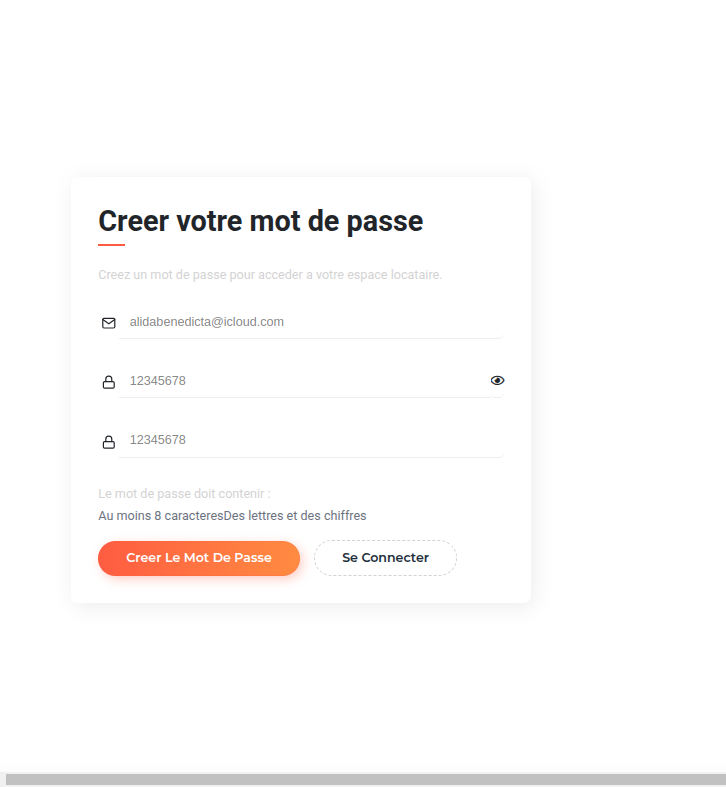
\includegraphics[width=\textwidth]{images/message-ges2.png}
	  \caption{ Création du mot de passe }
    \label{fig:prospect-fiche-bien}
\end{figure}


\begin{figure}[H]
    \centering
       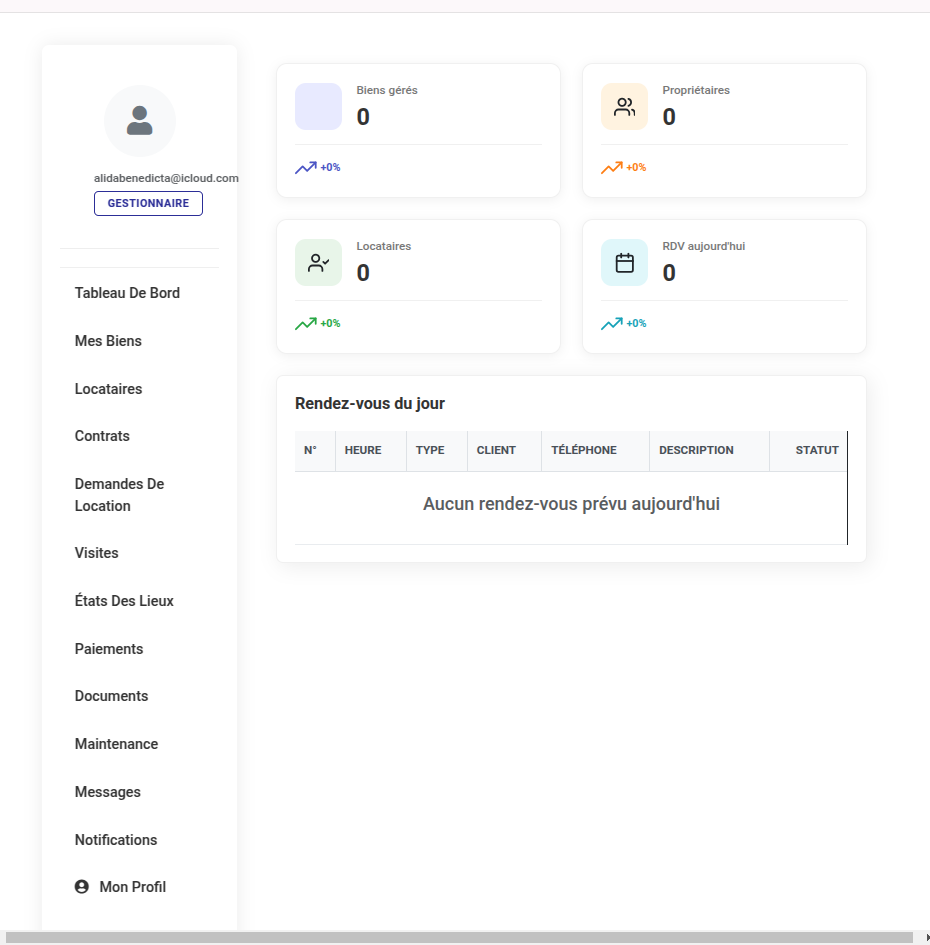
\includegraphics[width=\textwidth]{images/espace-ges.png}
	  \caption{ Accès au compte gestionnaire}
    \label{fig:prospect-fiche-bien}
\end{figure}



\vspace{0.3cm}

\begin{infobox}
\textbf{Administration des accès}

L'agence peut à tout moment \textbf{activer} ou \textbf{désactiver} un
gestionnaire depuis la liste de gestion, lui accordant ou lui retirant
l'accès à la plateforme selon les besoins opérationnels.
\end{infobox}


\begin{figure}[H]
    \centering
       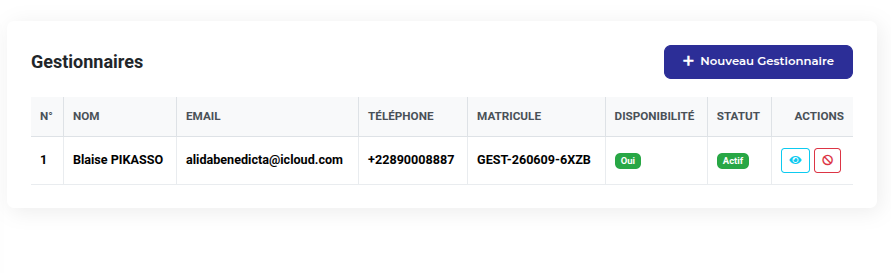
\includegraphics[width=\textwidth]{images/liste2.png}
	  \caption{ Création du mot de passe }
    \label{fig:prospect-fiche-bien}
\end{figure}




Les autres fonctionnalités du menu latéral de l'interface agence — 
gestion des biens, des visites, des contrats, des paiements, des 
incidents et des interventions suivent la même logique de gestion 
que celle décrite dans l'interface administrateur .






















\newpage
\subsection{Technologies utilisées}

La réalisation de la plateforme \motcle{IMMOBIZ} a nécessité le choix d'un ensemble d'outils et de technologies modernes, garantissant la performance, la sécurité et la maintenabilité du système. Le choix s'est porté sur une architecture de type \textit{Full-stack}.

\subsection{Technologies Frontend}

Le frontend représente l'interface utilisateur de l'application. L'objectif était de créer une expérience fluide, réactive et \textit{responsive} (adaptée aux mobiles).

\vspace{0.5cm}

% --- BLOC ANGULAR ---
\begin{minipage}{0.22\textwidth}
    \centering
    
\includegraphics[width=\textwidth]{images/angular_wordmark_gradient.png}
\end{minipage}
\hfill
\begin{minipage}{0.73\textwidth}
\begin{accentbox}
\textbf{Angular}

Développé par Google, Angular est un framework \textbf{SPA}  robuste. Contrairement à de simples bibliothèques, il offre un cadre de travail complet incluant la gestion des routes, des formulaires et des appels API. Son architecture basée sur les composants permet de réutiliser des éléments d'interface sur toute la plateforme \motcle{IMMOBIZ}.
\end{accentbox}
\end{minipage}

\vspace{0.8cm}

% --- BLOC TYPESCRIPT ---
\begin{minipage}{0.22\textwidth}
    \centering
    
\includegraphics[width=0.8\textwidth]{images/Typescript_logo_2020.svg.png}
\end{minipage}
\hfill
\begin{minipage}{0.73\textwidth}
\begin{accentbox}
\textbf{TypeScript (Langage natif)}

L'application a été entièrement développée en TypeScript, le langage de base d'Angular. En ajoutant un typage statique à JavaScript, il nous a permis de sécuriser le développement en détectant les erreurs de logique dès la phase de compilation.

\vspace{0.2cm}

\textbf{Avantages techniques :} L'utilisation du \textit{Data Binding} bidirectionnel et des \textit{Observables} (RxJS) assure une mise à jour en temps réel de l'interface, notamment lors de la recherche de biens immobiliers ou de la mise à jour des prix.
\end{accentbox}
\end{minipage}

\vspace{1cm}

\newpage

\subsection{Technologies Backend}

Le backend assure la gestion de la logique métier, la sécurité (authentification) et la communication avec la base de données. Pour ce projet, nous avons opté pour une architecture robuste et évolutive.

\vspace{0.5cm}

% --- BLOC SPRING BOOT ---
\begin{minipage}{0.22\textwidth}
    \centering
    
\includegraphics[width=\textwidth]{images/spring.png}
\end{minipage}
\hfill
\begin{minipage}{0.73\textwidth}
\begin{accentbox}
\textbf{Spring Boot}

Basé sur l'écosystème Java, Spring Boot a été utilisé pour créer une API REST performante. Il facilite le développement grâce à l'auto-configuration et sa gestion simplifiée des dépendances. C'est un framework qui garantit une grande sécurité et une facilité de test pour la plateforme \motcle{IMMOBIZ}.
\end{accentbox}
\end{minipage}

\subsection{Stockage des données}

Le stockage des données est un pilier central de la plateforme \motcle{IMMOBIZ}. Il doit garantir l'intégrité, la persistance et la sécurité des informations sensibles (utilisateurs, transactions, annonces).

\vspace{0.5cm}

% --- BLOC MYSQL ---
\begin{minipage}{0.22\textwidth}
    \centering
    
\includegraphics[width=0.85\textwidth]{images/mysql.png}
\end{minipage}
\hfill
\begin{minipage}{0.73\textwidth}
\begin{accentbox}
\textbf{MySQL}

Ce système de gestion de base de données relationnelle (SGBDR) a été choisi pour sa fiabilité et sa performance. Il permet de structurer les données de manière rigoureuse grâce à des relations entre les tables .

\vspace{0.2cm}

\textbf{Modèle Relationnel :} L'utilisation de MySQL facilite les requêtes complexes et garantit la cohérence des données grâce aux contraintes d'intégrité (clés étrangères).
\end{accentbox}
\end{minipage}

\vspace{0.8cm}

\section{Outils de développement}

L'utilisation d'outils collaboratifs et de plateformes modernes a été essentielle pour respecter les normes de qualité de l'entreprise \important{Synapses IT Solutions}.

\vspace{0.5cm}

% --- BLOC GIT / GITHUB ---
\begin{minipage}{0.22\textwidth}
    \centering
    
\includegraphics[width=0.75\textwidth]{images/github.png}
    \vspace{0.4cm}
    
    
\includegraphics[width=0.75\textwidth]{images/git.png}
\end{minipage}
\hfill
\begin{minipage}{0.73\textwidth}
\begin{infobox}
\textbf{Git \& GitHub}

Outils indispensables pour le versionnage du code source et la collaboration au sein de l'équipe de développement. Ils ont permis un suivi rigoureux des modifications via des branches dédiées.
\end{infobox}
\end{minipage}

\vspace{0.6cm}

% --- BLOC POSTMAN ---
\begin{minipage}{0.22\textwidth}
    \centering
    
\includegraphics[width=0.65\textwidth]{images/postman.png}
\end{minipage}
\hfill
\begin{minipage}{0.73\textwidth}
\begin{infobox}
\textbf{Postman}

Utilisé pour tester et valider les points d'accès (endpoints) de l'API REST développée avec Spring Boot avant leur intégration dans le frontend Angular.
\end{infobox}
\end{minipage}

\vspace{0.6cm}
% --- BLOC IDE ---
\begin{minipage}{0.22\textwidth}
    \centering
    
\includegraphics[width=0.40\textwidth]{images/vscode.jpeg}
\end{minipage}
\hfill
\begin{minipage}{0.73\textwidth}
\begin{infobox}
\textbf{VS Code}
Environnement de développement .
\end{infobox}
\end{minipage}

\vspace{0.6cm}

% --- BLOC OVERLEAF ---
\begin{minipage}{0.22\textwidth}
    \centering
    
\includegraphics[width=0.65\textwidth]{images/overleaf.png}
\end{minipage}
\hfill
\begin{minipage}{0.73\textwidth}
\begin{infobox}
\textbf{Overleaf (Édition LaTeX)}

Utilisé pour la rédaction du document et la mise en page du présent rapport. Cette plateforme permet une gestion rigoureuse de la documentation technique en utilisant le langage \LaTeX, garantissant ainsi un rendu professionnel .
\end{infobox}
\end{minipage}

\vspace{0.6cm}

% --- BLOC MERMAID ---
\begin{minipage}{0.22\textwidth}
    \centering
    
\includegraphics[width=0.65\textwidth]{images/mermaid_logo.png}
\end{minipage}
\hfill
\begin{minipage}{0.73\textwidth}
\begin{infobox}
\textbf{Mermaid (Modélisation)}

Outil de génération de diagrammes basé sur le concept du \textit{Diagram-as-Code}. Il permet de transformer des descriptions textuelles en représentations visuelles normées. Dans ce projet, il a été utilisé de manière générale pour garantir la rigueur des diagrammes UML et la cohérence entre la logique métier .
\end{infobox}
\end{minipage}

\vspace{0.6cm}

% --- BLOC MODELIO ---
\begin{minipage}{0.22\textwidth}
    \centering
    
\includegraphics[width=0.65\textwidth]{images/modelio.png}
\end{minipage}
\hfill
\begin{minipage}{0.73\textwidth}
\begin{infobox}
\textbf{Modelio} est l'outil de modélisation utilisé pour la conception du système. Il a permis de réaliser l'ensemble des diagrammes \textbf{UML}, notamment le diagramme de classes et les diagrammes de cas d'utilisation, garantissant ainsi une base solide avant la phase de développement.
\end{infobox}
\end{minipage}


\vspace{0.6cm}

% --- BLOC GESTION D'ÉTAT (STORE) ---
\begin{minipage}{0.22\textwidth}
    \centering
    
\includegraphics[width=0.65\textwidth]{images/store.png}
\end{minipage}
\hfill
\begin{minipage}{0.73\textwidth}
\begin{infobox}
\textbf{Gestion d'état (Store)} \\
L'architecture de l'application intègre un \textbf{Store} pour centraliser la gestion des données globales. Inspiré du pattern Redux, cet outil permet de maintenir une « source de vérité unique » pour l'état de l'interface \textbf{Angular}. Il facilite la synchronisation des données entre les composants (comme le panier de paiement ou le statut du dossier de location) tout en optimisant les performances et la traçabilité des actions utilisateur.
\end{infobox}
\end{minipage}



\vspace{0.6cm}
% --- BLOC SWAGGER ---
\begin{minipage}{0.22\textwidth}
    \centering
    
\includegraphics[width=0.65\textwidth]{images/swagger.png}
\end{minipage}
\hfill
\begin{minipage}{0.73\textwidth}
\begin{infobox}
\textbf{Documentation API (Swagger)} \\
L'application utilise \textbf{Swagger} pour documenter et tester l'ensemble des points des accès de l'API REST. Cet outil génère automatiquement une interface interactive permettant aux développeurs d'explorer les routes disponibles, de visualiser les modèles de données et d'effectuer des requêtes en temps réel. Il garantit une communication claire entre les équipes \textbf{front-end} et \textbf{back-end} tout au long du cycle de développement.
\end{infobox}
\end{minipage}


\vspace{0.6cm}

% --- BLOC MYSQL WORKBENCH ---
\begin{minipage}{0.22\textwidth}
    \centering
    
\includegraphics[width=0.65\textwidth]{images/mysqlbench.png}
\end{minipage}
\hfill
\begin{minipage}{0.73\textwidth}
\begin{infobox}
\textbf{Modélisation BDD (MySQL Workbench)} \\
La conception et l'administration de la base de données reposent sur \textbf{MySQL Workbench}. Cet environnement graphique permet de modéliser les schémas relationnels (tables, clés étrangères, contraintes), d'exécuter des requêtes SQL et de gérer les migrations de données. Il assure la cohérence du modèle de données pour des entités telles que les utilisateurs, les biens immobiliers ou les dossiers de location.
\end{infobox}
\end{minipage}



\subsection{Déploiement}

La mise en production de la plateforme \motcle{IMMOBIZ} repose sur une chaîne de déploiement automatisée combinant conteneurisation et intégration continue.

\vspace{0.5cm}

% --- BLOC CI/CD ---
\begin{minipage}{0.22\textwidth}
    \centering
    
\includegraphics[width=0.73\textwidth]{images/docker.png}
    \vspace{0.4cm}
    
\includegraphics[width=0.73\textwidth]{images/jenkins.png}
\end{minipage}
\hfill
\begin{minipage}{0.73\textwidth}
\begin{infobox}
\textbf{Docker \& Jenkins} \\
Le déploiement de la plateforme \motcle{IMMOBIZ} est automatisé grâce à \textbf{Jenkins} et \textbf{Docker}. Jenkins orchestre une chaîne d'étapes automatiques, appelée pipeline d'intégration et de déploiement continus (CI/CD — \textit{Continuous Integration / Continuous Deployment}), qui compile le code et vérifie sa qualité via SonarQube. \textbf{Docker} prend ensuite le relais en emballant l'application dans un conteneur isolé, garantissant qu'elle fonctionne de manière identique quel que soit le serveur sur lequel elle est déployée, qu'il s'agisse de l'environnement de développement ou de production.
\end{infobox}
\end{minipage}

\newpage

% ===============================
% CONCLUSION GÉNÉRALE
% ===============================
\chapter*{Conclusion générale}
\addcontentsline{toc}{chapter}{Conclusion générale}

\begin{highlightbox}
Ce projet de fin d'études a permis de concevoir et de développer \motcle{IMMOBIZ}, une plateforme de gestion immobilière répondant aux besoins identifiés lors de l'analyse du domaine. L'application offre une solution centralisée et efficace pour la gestion des biens, des utilisateurs et des transactions immobilières.
\end{highlightbox}

\vspace{0.4cm}

Le travail réalisé au sein de \important{Synapses IT Solutions} a constitué une expérience professionnelle enrichissante, permettant de mettre en pratique les connaissances acquises durant la formation à l'IFNTI. La démarche méthodologique adoptée, allant de l'analyse des besoins à la réalisation technique, a abouti à une solution fonctionnelle intégrant les technologies modernes du développement web.

\vspace{0.4cm}


\separateur

\begin{center}
    \textit{\textcolor{bleugris}{Ce projet constitue une base solide pour de futures évolutions et témoigne de l'importance de la digitalisation dans le secteur immobilier.}}
\end{center}




% ===============================
% RÉFÉRENCES & WEBOGRAPHIE
% ===============================
\newpage
\chapter*{Références et Webographie}
\addcontentsline{toc}{chapter}{Références et Webographie}

\begin{infobox}
Les sources suivantes ont été consultées pour l'analyse du contexte immobilier togolais ainsi que pour le choix des solutions technologiques.
\end{infobox}

\vspace{0.5cm}

\section*{Contexte du marché immobilier au Togo}

\begin{enumerate}[leftmargin=*, label={\textcolor{cuivre}{\textbf{[\arabic*]}}}]

    \item \textbf{République Togolaise} — \textit{Un marché immobilier en forte croissance}.\\
    Disponible sur : \url{https://www.republicoftogo.com/toutes-les-rubriques/eco-finance/un-marche-immobilier-en-forte-croissance}\\
    \textcolor{grisfonce}{Consulté en Avril 2026.}

    \vspace{0.3cm}

    \item \textbf{Afrilogement} — \textit{Défis et perspectives du secteur immobilier togolais}.\\
    Disponible sur : \url{https://afrilogement.com/article.php?id=55}\\
    \textcolor{grisfonce}{Consulté en Avril 2026.}

    \vspace{0.3cm}

    \item \textbf{République Togolaise} — \textit{Le marché immobilier a besoin de clarté}.\\
    Disponible sur : \url{https://www.republicoftogo.com/toutes-les-rubriques/eco-finance/le-marche-immobilier-a-besoin-de-clarte}\\
    \textcolor{grisfonce}{Consulté en Avril 2026.}

\end{enumerate}

\vspace{0.5cm}
\section*{Documentation Technique}

\begin{enumerate}[leftmargin=*, label={\textcolor{cuivre}{\textbf{[\arabic*]}}}, resume]

    \item \textbf{Spring Boot} — \textit{Documentation officielle (v3.x)}. \\
    Disponible sur : \url{https://spring.io/projects/spring-boot}\\
    \textcolor{grisfonce}{Consulté en septembre 2025.}

    \vspace{0.3cm}

    \item \textbf{Angular} — \textit{Guide officiel de développement web}. \\
    Disponible sur : \url{https://angular.io/docs}\\
    \textcolor{grisfonce}{Consulté en octobre 2025.}

    \vspace{0.3cm}

    \item \textbf{NgRx (Store)} — \textit{Reactive State Management for Angular}. \\
    Disponible sur : \url{https://ngrx.io/guide/store}\\
    \textcolor{grisfonce}{Consulté en octobre 2025.}

\end{enumerate}
\end{document}